% \documentclass[11pt,a4paper,twoside,openright,extrafontsizes]{memoir}

\renewcommand*{\baselinestretch}{1.025}
\isopage
\checkandfixthelayout

\newif\iftdkoneside
\tdkonesidefalse

%%% Local Variables:
%%% mode: latex
%%% TeX-master: "../main"
%%% End:

% We actually use `twoside` in oneside mode to avoid renumbering pages.
\documentclass[11pt,a4paper,twoside,extrafontsizes]{memoir}

\renewcommand*{\baselinestretch}{1.025}
\isopage
\setlrmargins{*}{*}{1}
\checkandfixthelayout

\newif\iftdkoneside
\tdkonesidetrue

%%% Local Variables:
%%% mode: latex
%%% TeX-master: "../main"
%%% End:


\usepackage{perpage}
\MakePerPage{footnote}

\usepackage{include/thesis}
\usepackage{enumitem}
\setlist{nolistsep}

\usepackage{rotating}

\usepackage{xcolor,colortbl}

\usepackage{listings}
\lstset{
	basicstyle=\small\ttfamily, % print whole listing small
	keywordstyle=\color{black}\bfseries, % bold black keywords
	identifierstyle=, % nothing happens
	commentstyle=\color{gray},
	showstringspaces=true,
	aboveskip=1em,
	belowskip=0.7em,
	columns=flexible,
	numbers=none,
	backgroundcolor=\color{white},
	extendedchars=false,
	inputencoding=utf8,
	xleftmargin=0em,
	xrightmargin=0em,
	framexleftmargin=0em,
	framextopmargin=0em,
	framexbottommargin=0em,
	frame=none,
	framerule=0pt,
	escapeinside={(*@}{@*)}
}


%
% General
%

\DeclareMathOperator*{\argmin}{arg\,min}
\DeclareMathOperator*{\argmax}{arg\,max}
\newcommand*{\dd}{\mathrm{d}}
\newcommand*{\T}{\mathrm{T}}
\newcommand*{\vecarrow}{}\let\vecarrow\vec
\renewcommand*{\vec}[1]{\bm{\mathrm{#1}}}

%
% Numbers
%

\newcommand*{\RR}{\mathbb{R}} % Reals
\newcommand*{\RRpos}{\RR^{+}} % Positiver reals
\newcommand*{\QQ}{\mathbb{Q}} % Rationals
\newcommand*{\ZZ}{\mathbb{Z}} % Whole numbers
\newcommand*{\NN}{\mathbb{N}} % Naturals
\newcommand*{\NNpos}{\NN^{+}} % Positive whole numbers

%
% Probability
%

\let\Pr\relax
\DeclareMathOperator{\Pr}{\mathbb{P}}
\DeclareMathOperator{\Ex}{\mathbb{E}}

%%% Local Variables:
%%% mode: latex
%%% TeX-master: "../main"
%%% End:


\newcommand*{\bme}{Budapest University of Technology and Economics}
\newcommand*{\vik}{Faculty of Electrical Engineering and Informatics}

\newcommand*{\bmemit}{Department of Measurement and Information Systems}

\newcommand*{\vikdoctype}{Bachelor's Thesis}
\newcommand*{\viktdklocation}{Budapest}
\newcommand*{\viktdkyear}{2017}

\newcommand*{\authors}{Authors}
\newcommand*{\advisors}{Supervisors}

\newcommand*{\authori}{Soma Lucz}
\newcommand*{\authorihun}{Lucz Soma}

\newcommand*{\advisori}{Dávid Honfi}

\title{Static analysis algorithms for JavaScript}
\newcommand*{\titlepagetitle}{Static analysis algorithms\\for JavaScript}
\author{\authori}

\hypersetup{
  pdftitle={\thetitle},
  pdfauthor={\theauthor, \advisors: \advisori}
}

%%% Local Variables:
%%% mode: latex
%%% TeX-master: "../main"
%%% End:


\newcommand{\es}{\mbox{ECMA}Script\xspace}

\bibliography{bibliography}
\addbibresource{bibliography.bib}

\setlength{\parskip}{8pt}
\setlength{\parindent}{0pt}

% source: https://github.com/steindani/msc-thesis/blob/master/src/main.tex
\lstdefinelanguage{JavaScript}{
  keywords={as, break, case, catch, continue, debugger, default, delete, do, else, export, finally, for, function, from, if, import, in, instanceof, let, new, return, switch, this, throw, try, typeof, var, void, while, with},
  morecomment=[l]{//},
  morecomment=[s]{/*}{*/},
  morestring=[b]',
  morestring=[b]",
  sensitive=true
}

% source: https://github.com/steindani/msc-thesis/blob/master/src/main.tex
\lstdefinelanguage{Rifle}{
  keywords={message, entityname, line, column, path},
  morecomment=[l]{//},
  morecomment=[s]{/*}{*/},
  morestring=[b]',
  morestring=[b]",
  sensitive=true
}

% source: https://github.com/steindani/msc-thesis/blob/master/src/main.tex
\lstdefinelanguage{Cypher}{
  morekeywords=[1]{BY, CREATE, DELETE, FOREACH, LIMIT, MATCH, MERGE, OPTIONAL, ORDER, REMOVE, RETURN, SET, SKIP, UNIQUE, WHERE, WITH, AND, OR, CONTAINS, DETACH},
	morekeywords=[2]{(, ), [, ], -(, )-, -[, ]-, --, ->, <-, -->, <--, )-->, )<--, -->(, <--(},
	keywordstyle={[2]\color{delim}},
  morecomment=[l]{//},
  morecomment=[s]{/*}{*/},
  morestring=[b]',
  morestring=[b]",
  sensitive=true,
	% literate=
	%  *{0}{{{\color{numb}0}}}{1}
	% 	{1}{{{\color{numb}1}}}{1}
	% 	{2}{{{\color{numb}2}}}{1}
	% 	{3}{{{\color{numb}3}}}{1}
	% 	{4}{{{\color{numb}4}}}{1}
	% 	{5}{{{\color{numb}5}}}{1}
	% 	{6}{{{\color{numb}6}}}{1}
	% 	{7}{{{\color{numb}7}}}{1}
	% 	{8}{{{\color{numb}8}}}{1}
	% 	{9}{{{\color{numb}9}}}{1}
}

\begin{document}

\frontmatter

\cleartorecto
\thispagestyle{empty}

\begin{tikzpicture}[overlay,remember picture]
  \node at (current page.center) [yshift=1cm] {%
    \begin{minipage}{\textwidth}

      \centering

      
\includegraphics[width=7cm]{include/figures/bme_logo}
      \vspace{0.3cm}

      \bme \\
      \vik \\
      \bmemit \\
      \vspace{3.5cm}

      {\Large \authori \par}
      \vspace{0.5cm}

      {\Huge\sffamily\bfseries \titlepagetitle \par}
      \vspace{1cm}

      {\large \vikdoctype \par}
      \vspace{3.5cm}

      {\Large 
        \advisors: \\ \vspace{0.3cm}
        \advisori\par}

      \vspace{1.5cm}
      {\large \viktdklocation, \viktdkyear\par}

    \end{minipage}};
\end{tikzpicture}

\cleardoublepage

%%% Local Variables:
%%% mode: latex
%%% TeX-master: "../main"
%%% End:


\tableofcontents

% Only needed for printing
% =====
% \cleartorecto
% \begin{otherlanguage}{magyar}

  \chapter*{Hallgatói nyilatkozat}
  \phantomsection
%  \addcontentsline{toc}{chapter}{Hallgatói nyilatkozat}
  \thispagestyle{plain}

  Alulírott \textbf{\authorihun} szigorló hallgató kijelentem, hogy ezt
  a szakdolgozatot meg nem engedett segítség nélkül, saját magam
  készítettem, csak a megadott forrásokat (szakirodalom, eszközök stb.)
  használtam fel. Minden olyan részt, melyet szó szerint, vagy azonos
  értelemben, de átfogalmazva más forrásból átvettem, egyértelműen, a
  forrás megadásával megjelöltem.

  Hozzájárulok, hogy a jelen munkám alapadatait (szerző(k), cím, angol
  és magyar nyelvű tartalmi kivonat, készítés éve, konzulens(ek) neve) a
  \textls{BME} \textls{VIK} nyilvánosan hozzáférhető elektronikus
  formában, a munka teljes szövegét pedig az egyetem belső hálózatán
  keresztül (vagy hitelesített felhasználók számára)
  közzétegye. Kijelentem, hogy a benyújtott munka és annak elektronikus
  verziója megegyezik. Dékáni engedéllyel titkosított diplomatervek
  esetén a dolgozat szövege csak 3~év eltelte után válik hozzáférhetővé.

  \vspace{4ex}

  \noindent Kelt: \viktdklocation, 2017. május 21.

  \vspace{20ex}

  \hfill\begin{minipage}{0.4\linewidth}
    \centering\hbox to \linewidth{\cleaders\hbox{.}\hfil}\par
    \centering\authorihun\par
  \end{minipage}

\end{otherlanguage}

%%% Local Variables:
%%% mode: latex
%%% TeX-master: "main"
%%% End:
% =====

\begin{otherlanguage}{magyar}

  \paragraph*{Kivonat}
  \phantomsection
  \addcontentsline{toc}{chapter}{Kivonat}
  \thispagestyle{plain}

  Szoftvereink kódját általában emberek írják. Az emberek általában hibákat követnek el, amik megfelelő eszköztárak hiányában felfedezetlenek maradhatnak. Ezen fejlesztői hibák fokozott kockázatot jelenthetnek a készülő szoftverre, hiszen az esetlegesen helytelen logikai működés mellett jelentős biztonsági réseket eredményezhetnek; kiaknázásuk a szoftver nemkívánatos viselkedését idézheti elő. Ez rosszindulatú támadóknak lehetőséget nyújthat arra, hogy a szoftvert számukra kedvező, az eredetileg tervezettől eltérő módon futtassák.

  A statikus forráskódanalízis egy az iparban gyakran használt, általánosan elfogadott szoftvertesztelési megközelítés. Mivel alkalmazásához a vizsgált kód lefuttatása nem szükséges, célja, hogy minél több szoftverfejlesztői hibát minél előbb, még a program fejlesztési szakaszában feltárjon, csökkentve ezzel a működés közben felmerülő programhibák számát, és így a telepítés utáni hibajavítással járó pluszköltségeket. Felhasználási lehetőségei közé tartozik a csoportos, vállalati kódolási szabályoknak, stílusoknak való megfelelés ellenőrzése, illetve egyre több szoftver nyújt támogatást egyre komolyabb logikai hibák fordítási vagy akár kódírási idejű feltárásához is.

  Napjaink folytonos integrációs infrastruktúrájába vagy fejlesztőkörnyezetbe illesztve a statikus analízis hatékony eszköz lehet a fejlesztői hibák feltárásában, és ezáltal állandó kódminőség biztosításában. Nagymértékű népszerűsége ellenére a JavaScript nyelvhez – annak dinamikus és gyenge típusosságából eredő sajátosságok következményeként – kevés statikus analízis-eszköztár létezik, és a rendelkezésre álló eszközök sem nyújtanak teljeskörű megoldást nagyméretű, vállalati szintű JavaScript forráskódtárak összefüggő elemzéséhez. Gyakran felmerülő probléma emellett az analitikus komplexitással általában fordítottan arányos sebesség: sem folytonos integrációs infrastruktúrába, sem fejlesztőkörnyezetbe nem illeszthető olyan eszköz, amely miatt a fordítási idő akár órákkal növekszik.

  Dolgozatomban egy már létező, a fenti követelményeknek nagy részben eleget tevő statikus kódanalízis-keretrendszer bővítését tervezem meg, fejlesztem le és értékelem ki. A bővítés során egyrészt új – logikai és formai – JavaScript-alapú statikus analízis-kikötéseket implementálok a rendszerhez. Másrészt lehetővé teszem, hogy a rendszer több összefüggő JavaScript-modulon (forrásfájlon) átívelő, globális analízis-kikötések kiértékelésére is képes legyen. Ezt kihasználva újabb kikötéseket implementálok, immáron több JavaScript-modult összefüggően elemző analízisekhez.

\end{otherlanguage}

\clearpage

\paragraph*{Abstract}
\phantomsection
\addcontentsline{toc}{chapter}{Abstract}
\thispagestyle{plain}

	Software codes are usually written by humans. Humans usually make mistakes, and in the absence of competent toolsets these human errors can remain undiscovered. Developer errors can be sufficiently dangerous: besides the improper logical operation of the software, they can lead to serious security vulnerabilities; exploiting them can cause the program to behave undesirably. This way, malicious attackers can take control over the software in some ways to run it according to their goals, or at least differently than originally intended.

	Static source code analysis is a widely used, generally approved software testing approach. As it does not require the software to be compiled and run, its goal is to discover and fix as many human errors as possible, as early as possible, meaning during development, in order to reduce the number of software failures in production and to minimize the extra costs of fixing bugs after deployment. Possible applications of static code analysis include verifying whether the code complies with enterprise coding standards and styles, but more and more analysis toolsets provide ways to detect more complex logical errors during compilation time, or even development time.

	In our days, static analysis toolsets integrated in Continous Integration (CI) workflows can be an efficient way to detect developer errors at commit- and build-time, and thus to provide constant code quality. Despite its widespread popularity, JavaScript does not have extensive static analysis tooling — a possible cause can be the language's dynamic and weak typing —, and either the existing tools do not provide a full-scale solution to globally analyse connected modules in large, enterprise-grade code repositories. Moreover, increased analysis complexity generally means significant reduction of speed, and of course a tool can not be integrated neither into a CI workflow, nor into a development environment, if it increases the build time with even several hours.

	In this thesis I design, implement and evaluate the extension of an existing static code analysis framework complying with most of the above detailed requirements. With the extension on the one hand, I implement new JavaScript static analysis constraints — logical and formal — for the framework. On the other hand, I extend the system with the capability of analysing more than one JavaScript source code files coherently, thus I provide a way to evaluate global analysis queries over more than one JavaScript modules related to each other. Then I implement more analysis constraints, but now for coherently analysing more than one, related JavaScript modules.

%%% Local Variables:
%%% mode: latex
%%% TeX-master: "main"
%%% End:


\mainmatter

\chapter{Introduction}

\section{Context}

Software development is a highly complex process involving many people, tools and methods. As the source code repository grows, code quality becomes an important aspect of the development procedure: as the software gets more and more complex, the number of human errors in the implementation gets higher. It is important to find and fix these errors as soon as possible: software defects found after deployment are 15 times more costly than if they were found during implementation.~\cite{dawson2010integrating} According to NIST, software bugs cost generally \$59.5 billion dollars for the US government annually.~\cite{tassey2002economic}

Today's generally used developer tools in commercial or significant open-source projects generally include \emph{version control systems (VCS)} and \emph{continuous integration (CI)} platforms.~\cite{hilton2016usage}~\cite{fowlerCI} Integrating \emph{code quality assurance} tools into the CI platform (or into the developer's \emph{integrated development environment (IDE)}) seems to be the practical choice for enforcing project-/company-wide coding style compliance, and to analyse the code deeper whether it contains defects.

A CI tool can be configured to scan and analyse the source code with external tools when the developer commits their code to the central code repository. A common workflow is the following:

\begin{enumerate}
\item the developer edits the code,
\item the developer commits the modified code into the central repository,
\item the VCS triggers a hook to inform the subscribers of the hook (including the CI platform) that new code has been committed,
\item the CI tool analyses the source code with the static analysis tools integrated and configured by the user, and creates a report about the analyses,
\item the CI tool builds the code and passes on the built artifact for testing and deployment.
\end{enumerate}

The reports created by the integrated static analysis tools give the developers insights about code quality and help them discover faults in the software before it gets to testing or production state.

We will focus on the static analysis of JavaScript projects. Although JavaScript is an interpreted language and thus generally considered not to require any building to be executed in browsers, it is still sensible to involve CI into JavaScript-projects for code quality and testing purposes, for a so-called transpiling\footnote{The procedure of transpiling will be detailed in Chapter 2.} step for the sake of compatibility, and for deployment.

\section{Problem Statement}

\section{Objectives and Contributions}

\section{Structure of the Thesis}

%%% Local Variables:
%%% mode: latex
%%% TeX-master: "../main"
%%% End:

\chapter{Preliminaries: Background}

This chapter presents the conception of static analysis, shortly summarises the JavaScript and its static analysis approaches to be detailed in Chapter 3, and gives insights to the previously mentioned background technologies of the \emph{Codemodel-Rifle} framework.


\section{Static Analysis}


\subsection{Introduction}

Static source code analysis is a widely used, generally approved~\cite{373902} software testing approach for analysing computer programs in as early as its source code state. It is performed without actually executing the program, meaning software can be analysed during development, before getting to the testing or deployment stage.

Static analysis techniques exist for almost 50 years.~\cite{emanuelsson2008comparative} A 1995 research paper concludes, that \textquote{Static analysis is effective and complementary to dynamic testing. Hence its use is to be recommended in the context of the majority of critical software.}~\cite{373902} In 2017, open- and closed-source static analysis tooling is quite extensive, and publicly available for not only the academia and the commercial industry, but for open-source projects as well.~\cite{wikipedia-static-analysis}

The sophistication and the generated reports' quality of static analysis tools vary: some report potential fault locations, others mathematically verify properties of a software and its specification. Besides general code quality-related applications, static analysis acquires a growing market share in safety- and mission-critical systems for exploring defects.~\cite{livshits2006improving}

In comparison with \emph{dynamic analysis}, static analysis is performed without compiling and executing the program itself. Usually statically analysed software source code is represented by a mathematical data structure, generally a tree or a graph, therefore the code needs to be transformed into an abstract data structure first.


\subsection{Source Code Transformation}

Software source code is a text, usually consisting of human-readable characters. Characters formulate sequences of instructions by the specified grammar of the programming language. To be executed on a computer, most programming languages need to be \emph{compiled} by a \emph{compiler} first, meaning the source code has to be transformed into a \emph{binary code} or \emph{bytecode} to be executed. Other languages, called interpreted languages, do not need to be compiled, they are interpreted and executed at runtime.\footnote{JavaScript is an interpreted language.}

Compiled languages' are always analysed, at least at compilation time by the compiler. If the software contains severe errors (like type association errors in strongly typed languages), the compiler will abort its operation, thus the software can not be run, since it has not been compiled. Considering interpreted languages do not need to be compiled, they are not analysed by a compiler before running, and, generally, not analysed at all. Interpreted languages' static analysis is therefore beneficial to compensate the lack of a compiler-like entity in the software processing chain.

Multiple static analysis methods can be run simultaneously on a project. As static analysis inspects the source code without modifying the original, the operations of several such tools are independent from each other. Therefore at compiled languages, added static analyses can only compliment the compiler's necessary analysis.

Usually three abstract data structures are used to represent software source code in a mathematically defined form.


\subsubsection{Abstract Syntax Tree (AST)}

If the compiler or an analysis tool processes the source code and its parser transforms the source code into an abstract data structure, it usually creates an \emph{Abstract Syntax Tree}. It is the tree-representation of the code, meaning every node in the tree is a semantic element of the source code. The \emph{source code to AST transformation} is vica versa unambiguous, meaning the two structures are identical to each other regarding the program logic. It is abstract in the sense of syntax: not all elements of the syntax is preserved in its AST, meaning without the language grammar, transformation would not be possible.


\subsubsection{Abstract Semantic Graph (ASG)}

A more abstract representation of the source code (or an AST) can be an \emph{Abstract Semantic Graph}. Derived semantic information added to the AST can result in a graph which provides more insights into the structure of the program: it can reveal data about variable and function scopes, and much more to be detailed later.


\subsubsection{Control-Flow Graph (CFG)}

Control-Flow Graphs or Execution Graphs contain execution path of a program. They are essential to compiler optimisations and widely used in static analysis tools.


\subsection{Use Cases and Limitations}

Static analysis use cases are generally code quality-related: on the one hand, the program under development should comply to specified programming styles and rules, on the other hand, the number of defects in the software should be as low as possible, ideally zero. If the software under development is part of a mission-critical solution, finding and fixing defects is essential.

Code style analysers and code formatters are used to enforce team- or company-wide coding styles. Linters are rule-based tools and are used to reveal simple programming errors and poorly used programming constructs. Pattern-matching techniques supplemented with algorithms to manipulate the representing data structure can be efficient to obtain deeper insights of the source code: this approach is to be detailed later being one of the subjects of this thesis. Static analysis with methods of formal verification uses mathematical models and methods to prove well-defined statements about the inspected source code.

Static analysis is limited in many ways. It often provides false values: \emph{false positives} are issues which do not have real significance or are not even true, \emph{false negatives} are real issues not being reported by the analysis tool. A framework is considered to be \emph{sound} if all defects checked for are reported by the tool: there are no false negatives but there can be false positives. A general approach of static analysis frameworks is to be sound, and simultaneously avoid extensive reporting of false positives.~\cite{emanuelsson2008comparative}

Regarding limitations, time and resources are also important aspects. An analysis tool can not be utilised efficiently, if the amount of either time or resources consumed by an analysis is too high. Even if it was theoretically possible to create a tool which finds every possible defects in a piece of source code, this tool would presumably consume so much time and resources for an analysis that there would be no appropriate use case for operating it.~\cite{anderson2008use}

Exploring execution paths greatly benefits static analysis proceedings, as it provides extra information about program states. Nevertheless, exploring all possible execution paths of a program is very costly: if a procedure contains $n$ branches without loops, the number of intraprocedural execution paths would be $2^n$.~\cite{anderson2008use} And even if a tool would encapsulate so much resources that it would be capable of exploring all possible executions paths, the set of possible inputs, whose cardinality is typically infinite, of the software would still not be taken into account. Since Alan Turing proved the halting problem to be generally undecidable over Turing-machines, we can conclude that, generally, some questions about a software can not be answered only by inspecting its source code.


\section{JavaScript}

JavaScript is a high-level, run-time interpreted language, featuring object-oriented capabilities. Being part of the core of the World Wide Web~\cite{flanagan2006javascript}, it is the most commonly used programming language in the world in 2016.~\cite{javascriptstackoverflow}


\subsection{Brief History of JavaScript}

Like all new technologies, JavaScript evolved very fast in the beginnings. The basics of the language was developed in 10 days by Brendan Eich, then-employee of Netscape Communications.~\cite{10.1109/MC.2012.57} The language had multiple names over the time: first it was Mocha, then LiveScript, then in December 1995, it was renamed to JavaScript as a sort-of marketing movement~\cite{webedjavascripthistory}, after seeing the then-popularity of Sun Microsystems' heavyweight Java language.

Initially, non-professional programmers were aimed by the idea to provide a portable, embeddable programming language that can be interpreted in web browsers. Since the syntax was closely similar to the syntax of C / C++ / Java, JavaScript rapidly gained traction: in the time of writing this thesis, it is the most used programming language in the world.~\cite{javascriptstackoverflow} It features browser-based client- and separate runtime-based server-side capabilities~\cite{nodejs} as well, and extensive tooling, package management~\cite{npmjs}, testing and build systems are available for automated operations in even larger software development organisations.


\subsection{The ECMAScript as a Standard and as a Language}

There is a significant aspiration to standardise the JavaScript language with its core capabilities and data structures. The first intentions of standardisation began in 1997 by Ecma International~\cite{webedjavascripthistory}, resuling in \emph{Standard ECMA-262}.~\cite{ecmascriptstandardfirstversion} The newest standard currently is the \emph{ECMA-262, 7\textsuperscript{th} Edition (ES7)}.~\cite{ecmascriptstandard} Apart from standardisation, there are several implementations of JavaScript in interpreters, e.g. Chakra\footnote{\texttt{https://github.com/Microsoft/ChakraCore}}, JScript\footnote{\texttt{https://msdn.microsoft.com/library/hbxc2t98.aspx}} and Google's V8\footnote{\texttt{https://github.com/v8/v8}}.~\cite{stein-daniel-msc}

Today's growing traction of standardised JavaScript, henceforth also referenced as ECMAScript, can be explained with several reasons. Due to being untyped\footnote{In JavaScript, no static types are assigned to entities.} and dynamic\footnote{Meaning of dynamic here: contrary to static languages where compilation time checks play an important role in verifying various properties of the program, dynamic languages' several common programming behaviours are executed only at run-time. Considering a common example: in JavaScript we have the \texttt{eval()} function to execute source code at run-time.}, static analysis of JavaScript is difficult. The ECMAScript standard enhances plain JavaScript with several new programming structures making the language more expressive and sometimes more simple.~\cite{es6-features} Users of the language can write more coherent code by applying these new language constructs as well as best practices making it easier to interpret the program by a static analysis tool.


\subsection{The Process of Transpiling}

\emph{Transpiling} is a word came into existence by mixing \emph{transforming} and \emph{compiling}. It is a generally used process in the ECMAScript developer community to ensure backwards compatibility of newer ECMAScript language standards, like ES6 and ES7.

\paragraph{Compiler}

A \emph{compiler} is a software with the primary goal of transforming software source code written in a high-level programming language into machine language, usually into a form of binary code called object code.~\cite{pcmagcompilers} Compiled languages, like C, C++, Java, or C\#, need to be compiled to be executed on a specific processor architecture.

\paragraph{Transpiler}

A \emph{source-to-source compiler} or \emph{transpiler} is a software which transforms software source code written in a high-level programming language into another high-level programming language. Ideally the two source codes are logically equivalent, meaning that with given abstractions, the operation of the two different software is the same.\footnote{The two executed programs need to be logically equivalent, but do not need to correspond in every technical aspects: there can be differences in machine-level operations and low-level proceedings.}

Transpiling and compiling have a set of common processing steps.~\cite{kulkarnitranspiler} First the source code is parsed into an abstract mathematical format for effective manipulation, then, after optimisations and transformations, both methods yield another kind of code. While compilers' output, being low-level machine code, can be generally executed on a computer architecture without further transformation steps, transpilers' output need further processing. Considering transpiling interpreted languages', the main use case is to provide compatibility with older or other versions of the language.

\begin{table}[!htbp]
	\newcommand{\fullsupport}{\tikz\draw[black,fill=black] (0,0) circle (0.8ex);\xspace}
	\newcommand{\partialsupport}{\tikz\draw[black,fill=none] (0,0) circle (0.8ex);\xspace}
	\newcommand{\nosupport}{—}
	\centering
	\begin{tabular}{l|cccc}
		\toprule
		                                    	&     \textbf{Chrome 58}     &     \textbf{IE 11}     &     \textbf{iOS 9}     &     \textbf{Android 5.1}     \\
		\midrule
		\textbf{default function parameters}  &     \fullsupport           &      \nosupport        &     \nosupport         &     \nosupport               \\
		\textbf{spread (…) operator}          &     \fullsupport           &      \nosupport        &     \partialsupport    &     \nosupport               \\
		\textbf{for..of loops}                &     \fullsupport           &      \nosupport        &     \partialsupport    &     \partialsupport          \\
		\textbf{const}                        &     \fullsupport           &      \partialsupport   &     \partialsupport    &     \partialsupport          \\
		\textbf{let}                          &     \fullsupport           &      \partialsupport   &     \nosupport         &     \nosupport               \\
		\textbf{arrow functions}              &     \fullsupport           &      \nosupport        &     \nosupport         &     \nosupport               \\
		\bottomrule
	\end{tabular}

	\caption{Excerpt from an ECMAScript 6 compatibility table~\cite{kangax}}
	\label{table:ecmascript-compatibility}
\end{table}

In the JavaScript scene, compatibility is a ubiquitous problem, see \Cref{table:ecmascript-compatibility}. Considering all the different browsers and server runtimes, and the slow progression of adopting JavaScript standards, transpiling has an important role in ensuring that the software works on a broad scale of platforms: code written in a modern syntax like ES6 can easily be transpiled into an universally supported syntax like plain JavaScript.

\Cref{fig:transpiling-example} shows two logically equivalent pieces of code: the second one (plain JavaScript) is created by transpiling the first one (ECMAScript 6) with a popular, automated transpilation tool, \emph{babel}\footnote{\texttt{http://babeljs.io}}. As the example shows, new language constructs can make the code much more concise, while the transpiled alternative provide compatibility with older desktop browsers and server runtimes.

\vspace{1em}
\begin{figure}[!htb]
	\centering
	\begin{minipage}{25em}
		The first piece of code uses ES6 constructs for simplicity:

		\begin{verbatim}
		[1, 2, 3].map(n => n ** 2);
		\end{verbatim}

		The second piece of code uses widely-supported plain JavaScript constructs only, and is created by transpiling the first piece of code with \emph{babel}:

		\begin{verbatim}
		[1, 2, 3].map(function (n) {
		  return Math.pow(n, 2);
		});
		\end{verbatim}
	\end{minipage}
  \caption{A transpilation example}
  \label{fig:transpiling-example}
\end{figure}


\subsection{Looking into the Goals of JavaScript Static Analysis}

As JavaScript is an interpreted language not being checked by a compiler by default at compilation time~\cite{373902}, it is recommended to apply static analysis during the development of, or before deploying a JavaScript application. Due to its dynamic and untyped\footnote{TypeScript, a strict superset of JavaScript adds static typing to the language.~\cite{typescript-website}} nature~\cite{flanagan2006javascript}, static analysis for the language is a challenging task. There are several existing approaches focusing mainly on defects detection~\cite{madsen2013practical, livshits2010gulfstream, jensen2009type}, but few of them are ready for production usage, and most of them lack compatibility with recent ECMAScript versions.

Being untyped, an obvious analysis goal is type inference: checking type correctness can eliminate several defects from software. Security demands imply that deeper, logical analysis of JavaScript code is needed. Besides security, the development procedure itself can also benefit from static analysis: there are features like automatic stub generation or auto-complete~\cite{madsen2013practical} in several development tools.~\cite{esprima-autocomplete, webstorm-autocomplete}


\section{Graph Databases}

Being graphs, developing new data structures for Abstract Syntax Trees, Abstract Semantic Graphs and Control-Flow Graphs would be superfluous: they can be practically stored in graph databases. There are established vendors on the open-source and also on the closed-source market~\cite{ibm-graph, arangodb-graph, datastax-graph, neo4j-website, orientdb-graph} providing databases with either a native graph storage model, or with support for storing graphs over an underlying data model other than a graph. For manipulating data, they provide well-defined and well-documented interfaces instead of ad-hoc solutions.

Graphs are mathematically well-defined data structures being broadly used in several fields of computer science. Recent technologies and implementations made possible for developers to easily embed graph data models into their applications. There are numerous real-world scenarios which can be represented more efficiently as graphs (\emph{nodes} connected to each other via \emph{edges}), than with the traditional, relational approach.

\subsection{The Property Graph Data Model}

It is a common way to define graphs as a set of objects, in which some object pairs are connected to each other. In this model, an object is called \emph{vertex} or \emph{node} or \emph{point}, and a connection between two \emph{vertices} is called \emph{edge} or \emph{relation}. Connections can be detailed further by specifying their directionality, also they can be \emph{labeled} to define them even more. Similarly labeling vertices leads to the model of \emph{typed graphs}. If we assign properties to the nodes or relations, we get the model of \emph{property graphs}. Properties, as shown in \Cref{fig:property-graph}, are usually key-value pairs in the format of \texttt{key = `value'}. Generally, keys are strings, and values represent common data types like string, integer, float, etc.

\begin{figure}[!htb]
	\centering
	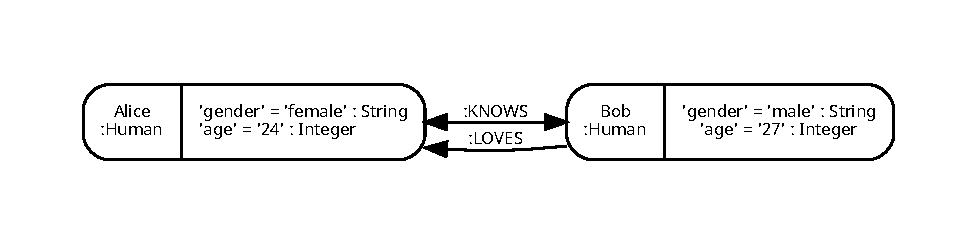
\includegraphics[width=\textwidth, trim=1cm 1cm 1cm 1cm,clip]{figures/property-graph.pdf}
	\caption{Two people's relationship modeled with a property graph}
	\label{fig:property-graph}
\end{figure}

The Codemodel-Rifle framework uses property graphs for its internal data storage. The parsed source code's AST is transformed into an ASG, and is stored as a property graph: nodes in the AST become property graph nodes, nested AST nodes are connected to each other via labeled graph relations. \Cref{fig:codemodel-rifle-asg} shows the ASG of the following JavaScript program: \texttt{const PI = 3.141593;} produced and visualised by Codemodel-Rifle.\footnote{Administrative properties and labels are omitted for the sake of simplicity, e.g. no identifiers are shown.}

\begin{figure}[!p]
	\centering
	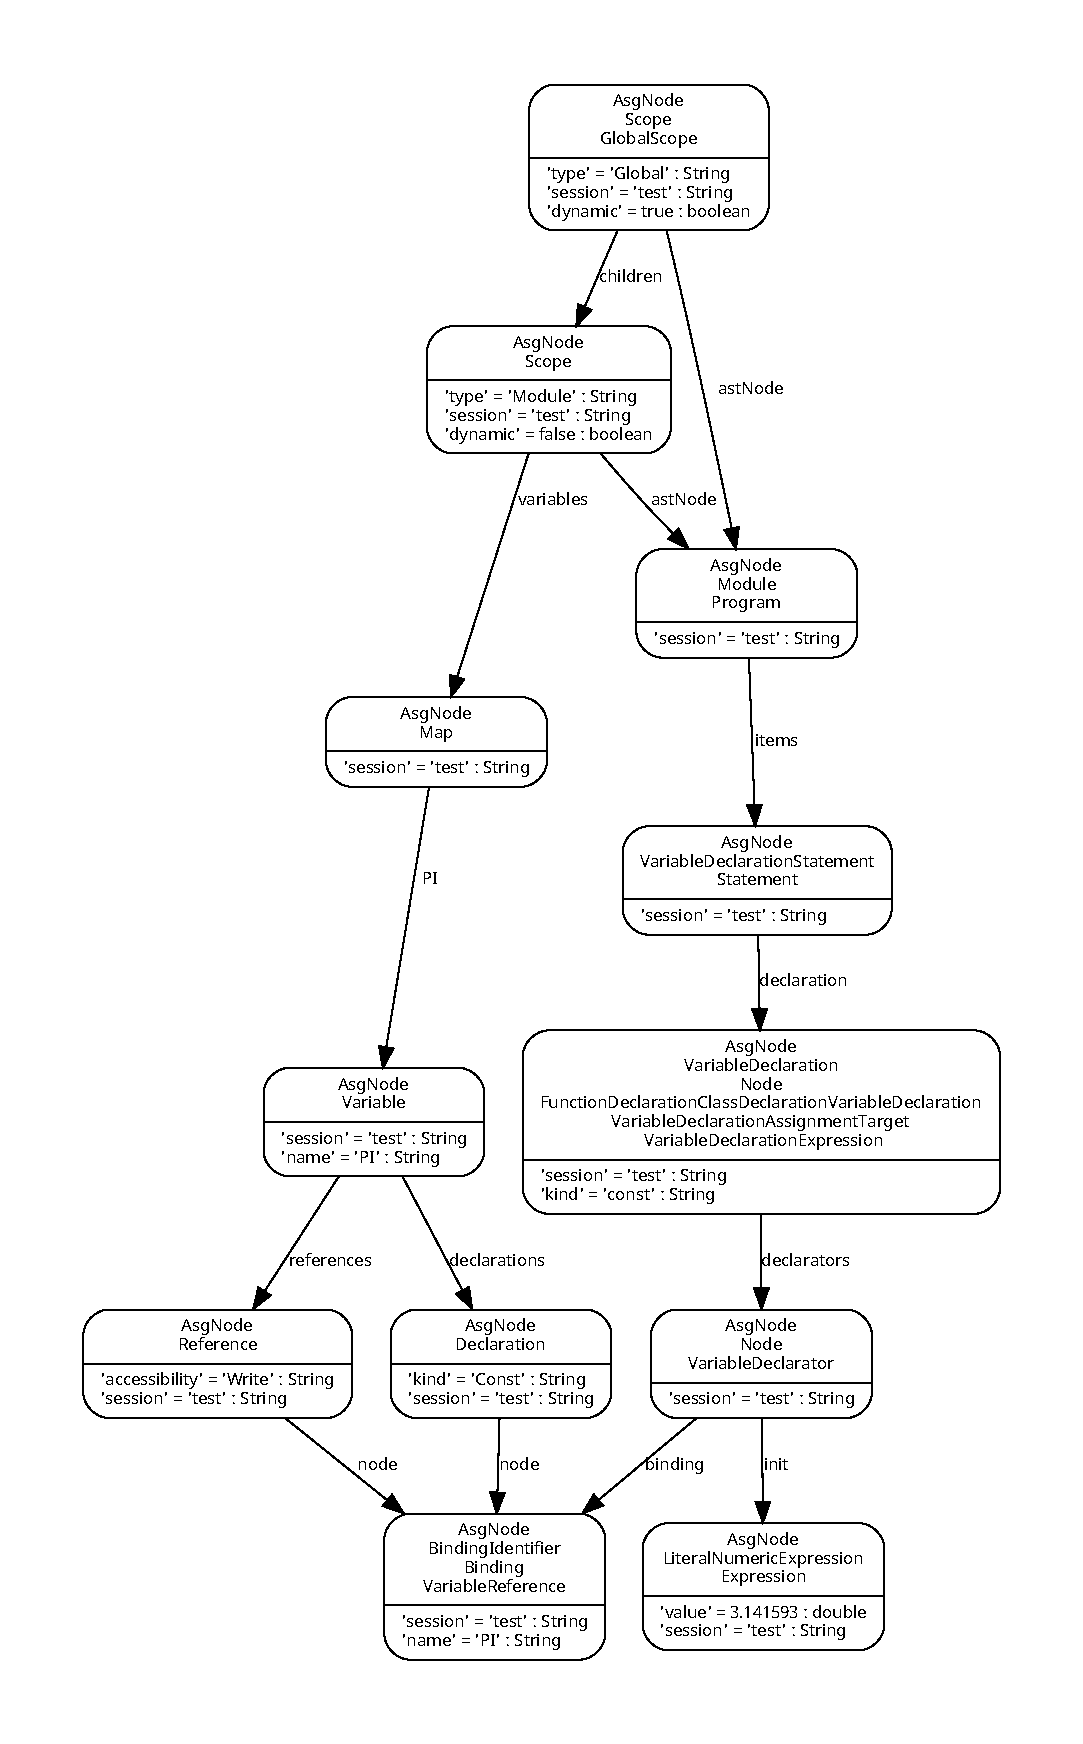
\includegraphics[height=\textheight, trim=1cm 1cm 1cm 1cm,clip]{figures/codemodel-rifle-asg.pdf}
	\caption{\texttt{const PI = 3.141593;} in Abstract Semantic Graph format}
	\label{fig:codemodel-rifle-asg}
\end{figure}

\subsection{Neo4j}

Amongst a handful of graph database vendors~\cite{graph-dbs}, Neo Technology's Neo4j is the most popular~\cite{graph-dbs-raking} one. It features a pure graph data model, contrary to other vendors' multi-model approaches. Besides Neo Technology, Neo4j is backed by the open-source community as well.~\cite{neo4j-github} There are two variants: \emph{Community Edition} and \emph{Enterprise Edition} with an extended feature set. Interestingly, open-source licensing is available for the Enterprise Edition as well~\cite{neo4j-opensource}, for closed-source software, commercial licensing is available~\cite{neo4j-licensing}.

Neo4j provides two access models, detailed in the following paragraphs.

\paragraph{Embedded mode} For JVM-based languages, a native API is exposed for data operations with a very low latency. This makes the database directly embeddable to any software written in a JVM-compatible language, but provides less scalability than the \emph{server mode}.

\paragraph{Server mode} The database can be operated as a separate server listening on its binary \emph{Bolt} protocol as well as on its HTTP REST interface. From scalability aspects, the Enterprise Edition's master-slave database replication\footnote{At the time of this writing, multi-master replication is not offered by Neo4j.~\cite{neo4j-clustering-architecture}} is only available in server mode.

The Codemodel-Rifle framework uses Neo4j for its property graph storage. At first, the database was embedded into the software, but due to licensing issues, the framework had to be refactored to use Neo4j in server mode.\footnote{The licensing issues and the details and results of the refactoring are described in Section 3.1.}

\subsection{Cypher}

Cypher is a query language developed especially for graph databases by Neo Technology.~\cite{neo4j-cypher} Contrary to the usage of the native API, it is mostly used when Neo4j is deployed in server mode. \Cref{fig:cypher-intro} shows that the language uses a sort of ASCII-art to represent nodes and relationships: nodes are in parentheses, relationships are in brackets surrounded by relationship direction information.

\begin{figure}[!htb]
	\centering
	\texttt{(Bob)-[:LOVES]->(Alice)}
  \caption{A basic Cypher example}
	\label{fig:cypher-intro}
\end{figure}

Cypher syntax is elegant and expressive, thus very readable. Besides using it to represent nodes and relationships, we can utilise it to access the database's indexing capabilities and stored procedures. Since complex pattern-matching conditions can be expressed easily and intuitively in Cypher, it should be the primary way of accessing Neo4j instead of the little bit faster but less readable API.\footnote{Since the subject of this thesis mainly features Cypher queries, Cypher is detailed further in Chapter 5.}


\section{Running Example}

In this section I provide a set of ECMAScript codes as a software defect example, which accompanies the reader throughout the thesis. This example is to be used whenever a new static analysis concept is introduced. There are two files in the example: \texttt{exporter.js} and \texttt{importer.js}.

The first one exports a function, which happens to return $0$, as a variable. The second one imports the variable and tries to divide a number with the return value of the imported function variable. Through this example, I present that this and similar software defect cases can be revealed by static analysis, even if the defect spans multiple ECMAScript modules (source files), and includes patterns which can not be matched by one generalised pattern description. \Cref{fig:running-example-exporter} presents \texttt{exporter.js}. \Cref{fig:running-example-importer} presents \texttt{importer.js}.

\vspace{2em}
\begin{figure}[!htb]
	\centering
	\begin{minipage}{25em}
		\begin{verbatim}
		var a = 0;

		export default function b() {
		  let c = function d() {
		    return a;
		  };

		  return c();
		};
		\end{verbatim}
	\end{minipage}
  \caption{\texttt{exporter.js} module}
  \label{fig:running-example-exporter}
\end{figure}

\vspace{2em}
\begin{figure}[!htb]
	\centering
	\begin{minipage}{25em}
		\begin{verbatim}
		import defaultName from "exporter";

		let a = 5 / defaultName();
		\end{verbatim}
	\end{minipage}
  \caption{\texttt{importer.js} module}
  \label{fig:running-example-importer}
\end{figure}

%%% Local Variables:
%%% mode: latex
%%% TeX-master: "../main"
%%% End:

\chapter{Related Work}
\label{chapter:relatedwork}

This chapter specifies the currently known approaches and related work of static analysis in general, and specifically for JavaScript.


\section{Static Analysis Tools for JavaScript}

This section introduces several static analysis tools for the main subject of this thesis, the JavaScript language.


\subsection{TAJS (Type Analysis for JavaScript)}

TAJS is a static data flow analysis tool for JavaScript with the capability of inferring detailed and sound type information using abstract interpretation~\cite{jensen2009type}. In the time of this writing, it fully supports the 3\textsuperscript{rd} version of \es, and partially supports the 5\textsuperscript{th} version\footnote{\es 5 is the most popular, and most broadly used version of \es, supported by most of the desktop and mobile browsers and external runtimes~\cite{kangax-es5}. This is the \es version I referred to previously as \emph{plain JavaScript}.}, including its standard library, the HTML DOM, and the browser API~\cite{tajs-github}.

The abstract interpretation approach consists of the following main points~\cite{tajs-presentation}:

\begin{enumerate}
\item construct the \emph{Control-Flow Graph} of the program,
\item define a data flow lattice~\cite{jensen2009type}, which abstracts program data flow into a mathematically interpreted format,
\item define transfer functions, which abstracts the operations on the data flow lattice.
\end{enumerate}

There is an Eclipse plug-in for TAJS, but it is not ready for production usage, according to the creators of the framework~\cite{tajs-website}.


\subsection{Flow}

Flow is a static type checker for JavaScript developed and maintained by the Facebook Open Source community~\cite{flow-github}. Flow checks the code for defects based on \emph{static type annotations}~\cite{flow-website}. Without explicit type annotations, Flow is still able to work by attempting to infer types implicitly. Thus, into larger codebases, Flow can be introduced incrementally.

Like many other static analysis tools, Flow also aims for soundness, while preventing extensive reporting of false positives. The developers of the tool identified two main goals: precision and speed. According to the very imprecise documentation~\cite{flow-docs}, Flow is made to be practically precise by modeling the language's essential characteristics accurately enough to differentiate between intentional solutions and unintentional mistakes.

Flow's speediness means to be part of the editing process: the goal is to be fast enough for an IDE to show type information in real-time, during editing the code. To achieve this speed, Flow uses incremental processing with file-granularity, meaning only the changes since the last analysis need to be processed.

\subsection{Tern}

From the Tern website: \textquote{Tern is a stand-alone code-analysis engine for JavaScript. It is intended to be used with a code editor plugin to enhance the editor's support for intelligent JavaScript editing.}~\cite{tern-website}

Tern provides features like editor auto-completion of variables and properties, function argument hints, automatic refactoring, and finding the definition of a function or variable. It is written in JavaScript, and capable of running both on node.js and in the browser.

The software is maintained on GitHub~\cite{tern-github} by Marijn Haverbeke, developer of the Acorn lightweight JavaScript parser. Acorn is used as the underlying parser for the Tern infrastructure, which consists of several components: the editor plugins communicate with the Tern server, which is implemented on top of the server module, which uses the inference engine to perform analyses~\cite{tern-website}.

Editor plug-ins' list contains editors with significant or growing popularity:

\begin{itemize}
\item Emacs
\item Vim
\item Sublime Text
\item Brackets
\item Eclipse
\end{itemize}

At the time of this writing, the newest version of Tern is $0.21$, implying that the tool is not yet aimed for heavyweight production usage, but rather for experimental purposes.


\subsection{Shift}

Shift is not a static analysis tool, but an AST toolset created and developed by Shape Security, consisting of several tools~\cite{shift-ast}. Besides others, Shift features a parser, a code generator, and a scope analyser. It supports the full \emph{\es 7\textsuperscript{th} Edition}~\cite{shift-ast}, and its parser and scope analyser are foundations of the Codemodel-Rifle framework.

It is to be mentioned here, that Shift uses its own AST format, first announced by Shape Security in late 2014, as their first open-source contribution. According to their reasoning, a new \es AST format was needed because its predecessor, Mozilla's SpiderMonkey AST was not specifically created for static analysis purposes, but rather for an internal representation only for interpretation.

Shift AST is said to comply with all aspects of a good AST-format, as

\begin{itemize}
\item \textquote{it minimizes the number of inhabitants that do not represent a program,
\item it is at least partially homogenous to allow for a simple and efficient visitor,
\item it does not impede moving, copying, or replacing subtrees,
\item it discourages duplication in code that operates on it.}~\cite{shift-ast-comparison}
\end{itemize}

\subsection{Esprima}

Esprima is an \es parser with extended capabilities, like syntax validation. It supports the full standard of \emph{\es 7\textsuperscript{th} Edition}. The open-source software is created by Ariya Hidayat, engineer of \emph{Shape Security}, and is maintained on GitHub.


\subsection{Comparison of the Featured Tools}

\begin{table}[!htb]
	\newcommand{\fullsupport}{\tikz\draw[black,fill=black] (0,0) circle (0.8ex);\xspace}
	\newcommand{\partialsupport}{\tikz\draw[black,fill=none] (0,0) circle (0.8ex);\xspace}
	\newcommand{\nosupport}{—}
	\centering
	\begin{tabular}{l|ccccc}
		\toprule
																					&   \textbf{TAJS}   &   \textbf{Flow}   &   \textbf{Tern}   &   \textbf{Shift Java}   \\
		\midrule
		\textbf{\es support}           &   ES3             &   ES5             &   ES6             &   ES7                   \\
		\textbf{AST-format}                   &   \nosupport      &   \nosupport      &   SpiderMonkey    &   Shift                 \\
		\textbf{open-source}                  &   \fullsupport    &   \fullsupport    &   \fullsupport    &   \fullsupport          \\
		\textbf{number of contributors}       &   1               &   335             &   87              &   10                    \\
		\textbf{license}                      &   Apache 2.0      &   BSD 3           &   MIT             &   Apache 2.0            \\
		\textbf{current version number}       &   v0.9-10         &   v0.45.0         &   0.21.0          &   es2016-v1.1.1         \\
		\midrule
		\textbf{infers types}                 &   \fullsupport    &   \fullsupport    &   \fullsupport    &   \nosupport            \\
		\textbf{needs non-standard syntax}    &   \nosupport      &   \fullsupport    &   \nosupport      &   \nosupport            \\
		\textbf{analyses related files}       &   \nosupport      &   \nosupport      &   \fullsupport    &   \nosupport            \\
		\bottomrule
	\end{tabular}

	\caption{Comparison of the featured JavaScript static analysis tools}
	\label{table:javascript-tools-comparison}
\end{table}


\section{Static Analysis Tools for Java}

This section introduces static analysis tools for Java, mainly for earning new ideas regarding static analysis.


\subsection{FindBugs}

FindBugs is a static analysis tool for detecting bug patterns in Java code~\cite{findbugs-website}. One of its main techniques is to syntactically match source code to programming constructs marked as suspicious programming practise. \textquote{For example, FindBugs checks that calls to \texttt{wait()}, used in multi-threaded Java programs, are always within a loop–which is the correct usage in most cases. In some cases, FindBugs also uses dataflow analysis to check for bugs. For example, FindBugs uses a simple, intraprocedural (within one method) dataflow analysis to check for null pointer dereferences. FindBugs can be expanded by writing custom bug detectors in Java. We set FindBugs to report \textquote{medium} priority warnings, which is the recommended setting.}~\cite{rutar2004comparison}


\subsection{PMD}

Similarly to FindBugs, PMD performs syntactic analysis on Java programs, but is does not have a data flow component. \textquote{In addition to some detection of clearly erroneous code, many of the \textquote{bugs} PMD looks for are stylistic conventions whose violation might be suspicious under some circumstances. For example, having a try statement with an empty catch block might indicate that the caught error is incorrectly discarded. Because PMD includes many detectors for bugs that depend on programming style, PMD includes support for selecting which detectors or groups of detectors should be run.}~\cite{rutar2004comparison}


\subsection{jQAssistant}

A German technology firm, Buschmais developed a component-based static analysis tool for Java, called jQAssistant~\cite{jqassistant-website}. Similarly to the Codemodel-Rifle framework, jQAssistant is built upon the Neo4j graph database. According to the documentation~\cite{jqassistant-documentation}, the tool is to be integrated into the build process to detect constraint violations and generate reports about user defined concepts and metrics.

Analysis rules can be expressed in Neo4j's graph query language, Cypher. However, instead of the semantics of the source code itself, jQAssistant focuses on the software components and their connections. Its features include validating dependencies between modules in a project, enforcing naming conventions e.g. for test classes, packages, JPA entities, and detecting common architectural problems like cyclic dependencies~\cite{jqassistant-documentation}. The products is licensed under GNU General Public License, v3, allowing developers to use it in open-source projects~\cite{gplv3}.


\section{Static Analysis Tools for C and C++}

This section introduces static analysis tools for C and C++, mainly for earning new ideas regarding static analysis.


\subsection{Clang}

Besides serving as a compiler front-end for LLVM, Clang has a static analyser component for finding bugs in C, C++, and Objective-C programs~\cite{clang-analyser-website}. The tool can be used either as a standalone command-line tool, or as an Xcode\footnote{Xcode is Apple's integrated development environment only available for Apple's macOS, containing a suite of development tools for Apple platforms: macOS, iOS, watchOS and tvOS.} plugin.

Clang uses static analysis based on compiler techniques. It is designed to report much more information than GCC, using control-flow graph analysis. It features flow- and path-sensitive analyses while preserving the overall form of the original source code~\cite{kremenek2008finding}. The tool can be integrated into IDEs, and supports automated refactoring.


\subsection{PolySpace}

PolySpace Technologies, which first developed the PolySpace Verifier static analysis tool, was later acquired by MathWorks. PolySpace Verifier has been reorganised into a suite, which now features static analysis for C and C++. Similar to TAJS's approach, PolySpace uses the classic lattice-theoretic abstract interpretation technique. The underlying analyser relies on a sound approximation of the set of all reachable states~\cite{emanuelsson2008comparative}. The tool features a mathematical data structure named \emph{convex polyhedron}\footnote{A convex polyhedron is an $n$-dimensional geometric shape where for any pair of points inside the shape the straight line connecting the points is also inside the shape~\cite{emanuelsson2008comparative}.}, multiple \emph{convex polyhedra} encodes the sets of states~\cite{cousot1978automatic}.

The tool is sound in the meaning that, given the full code base of the project, it computes the superset of every reachable state. It is flow-sensitive, context-sensitive, features inter-procedural analyses, and supports aliasing. \textquote{The properties checked by PolySpace Verifier are in many cases similar as those checked e.g. by other commercial systems, but the analysis is more sophisticated taking account of non-trivial relationships between variables (taking advantage of convex polyhedra) while other static analysis tools seem to cater only for simple relationships (e.g. equalities between variables and variables being bound to constant values or intervals of values).}~\cite{emanuelsson2008comparative}

PolySpace Verifier features checks for array conversion range extensions, return value initializations, variable initializations, pointer initializations, scalar/float under- and overflows and division by zero, non-termination of calls and loops, correctness of function arguments, unreachable code and many others~\cite{emanuelsson2008comparative}.

In today's product portfolio~\cite{polyspace-website}, Polyspace Bug Finder™ features the goal of locating defects with static analysis, and Polyspace Code Prover™ is said to prove the absence of run-time errors in C and C++ source code.


\subsection{Coverity}

Coverity Prevent, now part of Synopsys~\cite{coverity-website}, is a static analysis tool created as a spin-off from a research group at Stanford University. \textquote{In 2006 Coverity and Stanford were awarded a substantial grant from the U.S. Department of Homeland Security to improve Coverity tools to hunt for bugs and vulnerabilities in open-source software. During the first year 5,000 defects were fixed in some 50 open source projects. Updated results of the analyses can be found on the web.

The tool itself is a data-flow analysis tool featuring inter-procedural analyses. The analysis is neither sound nor complete, that is, there may be both defects which are not reported and there may be false alarms. A substantial effort has however been put on eliminating false positives, and the rate of these is clearly low (reportedly around 20 per cent).}~\cite{emanuelsson2008comparative}

Coverity features a different set of C and C++ checkers. For C, Coverity checks for resource leaks, dereferencing/deallocating already deallocated memory, uninitialised variables, unused pointer values, dead code, null pointer dereferences, misuse of negative integers and functions that may return negative integers, and null returns, amongst others. For C++, Coverity checks for errors in overriding virtual functions, resource leaks because of missing destructors, past-the-end STL iterators, and uncaught exceptions, amongst others.

Coverity has concurrency and security checkers as well, such as checks for double locks and missing releases, dangerous function calls like \texttt{gets} or \texttt{strcpy}, string overflows, and incorrect usage of the \texttt{chroot} system call~\cite{emanuelsson2008comparative}.


\section{Most Used Error-Checking Constraints}

According to the above related work, the following error-checking constraints are the most widely used ones in static analysis tools:

\begin{itemize}
\item type correctness,
\item uninitialised variables,
\item unreachable code,
\item division by zero,
\item misuse of negative integers as function arguments.
\end{itemize}

\chapter{Overview of the Approach}
\label{chapter:overview}

This chapter gives an overview of my approach of JavaScript static analysis using the \emph{Codemodel-Rifle} framework.


\section{Refactoring the Codemodel-Rifle Framework}

Dániel Stein, creator of the Codemodel-Rifle framework, details the design of the framework in his Master's Thesis~\cite{stein-daniel-msc}. Following his thesis and my experiences with the framework, the summary of the software's architecture is the following:

\begin{itemize}
\item A source code file is to be delivered to Codemodel-Rifle via the HTTP REST API of the framework's embedded webserver as a text.
\item The framework parses the incoming source file into an AST model with Shape Security's Shift parser.
\item The framework performs scope analysis on the AST model with Shape Security's scope analyser, transforming the AST model into an ASG model.
\item The ASG model is transformed to a property graph and is stored in the framework's embedded Neo4j graph database.
\item Apart from importing a file, the framework is able to perform analyses on or visualisation of a graph stored in its database, if requested over its REST API.
\item Analysing multiple \es files are minimally supported by interconnecting related modules' subgraphs along the \emph{export} and \emph{import} \es statements, but not all use cases and combinations are implemented.
\item The result of the analyses or the visualisation is returned via the REST API in JSON or in a visual file format.
\end{itemize}

Codemodel-Rifle was notably refactored since the state of the above summarised architecture. This section introduces why refactoring was necessary, and presents the details and the results of the process.


\subsection{Open-Sourcing and Licensing Issues}

Development of the Codemodel-Rifle framework was supported by the Fault-Tolerant Systems Research Group (FTSRG) of the Budapest University of Technology and Economics. FTSRG's decision (with the support of Dániel Stein) was to open-source the framework under FTSRG's name. According to an agreement with the university, FTSRG can only release open-source code under the Eclipse Public License, version 1.0 (EPLv1)~\cite{eplv1}. As it is maintained by the FTSRG, the Codemodel-Rifle framework is required to be released under EPLv1, if open-sourced. This introduced several licensing problems~\cite{codemodel-rifle-licensing}.

The framework uses Neo4j as its internal graph data storage, and Neo4j was embedded into Codemodel-Rifle~\cite{stein-daniel-msc}. From the point of licensing, there is an important difference between \emph{using} the database \emph{via a network connection} and \emph{embedding} the database \emph{into software}. Since Neo4j's Community Edition, used by Codemodel-Rifle, is licensed under GPLv3~\cite{neo4j-licensing}, it can be used remotely via a network connection with practically any license because of the so-called \emph{application service provider loophole}~\cite{asp-loophole}, but it can not be embedded into applications which do not comply with GPLv3. As EPLv1 and GPLv3 are incompatible, Neo4j can not be embedded into the open-sourced Codemodel-Rifle.

Consequently, a necessary step was to switch from embedded Neo4j to remote Neo4j accessed via a driver. But, as native API-calls, which were extensively used by Codemodel-Rifle, can not be used with driver-accessed remote Neo4j, this caused further problems; these are subjects of the next subsections.


\subsection{Decomposing the Architecture}

Codemodel-Rifle's first architecture was a monolith. It \emph{embedded} four key modules:

\begin{itemize}
\item a Neo4j graph \textbf{database},
\item a \textbf{webserver} exposing an HTTP REST API for interactions,
\item the \textbf{core module} responsible for transforming source code into an ASG and performing analyses on the graph,
\item and \textbf{other application logic}, e.g.\ for displaying and exporting AGSs into visual file formats like PDF or PNG.
\end{itemize}

Decoupling, or minimising direct interdependencies between components is an important aspect of software engineering. If a software is decomposed into smaller components along well-defined interfaces, it becomes modular: any module's inner functioning can be changed without affecting other modules, as long as the module implements the interface it was bound to. Motivations to alter a module include performance issues, scalability efforts, or changed domain logic. Codemodel-Rifle's first architecture was well-designed for easy manual testing and seemed to be an obvious solution for creating a small-scale graph-based analysis software. However, demands like simultaneous usage of multiple users, or having dedicated hardware resources to run analysis queries over large repositories, required the Codemodel-Rifle framework to become modular to adapt.


\subsubsection{Detaching the Database}

Apart from the licensing issues detailed above, using a remote Neo4j server as a database instead of the embedded version comes with several benefits. The database can be outsourced onto a separate hardware or infrastructure: since analyses and graph maintenance can be demanding over large code repositories, providing dedicated resources for the database is an obvious solution for possible performance issues and scalability.

With a remote Neo4j database, a custom database driver can be utilised. This driver can be capable of incremental processing on the graph database level\footnote{Gábor Szárnyas is developing a graph database driver \emph{ingraph} with the goal of evaluating openCypher queries incrementally~\cite{ingraph-github}.}, or it can support testing by providing an in-memory database instance via a driver\footnote{The default configuration of the framework is to use an in-memory Neo4j database currently. This is to be detailed in the next subsection.}.

As a result of the aforementioned benefits and licensing issues, the framework was refactored to use a remote Neo4j server via a driver. This meant native API-calls were no longer possible: interacting with the database has been restricted to Cypher queries provided via the database driver. The Codemodel-Rifle framework extensively used native API-calls, so all these function calls had to be rewritten into distinct Cypher queries. As Cypher queries turned out to be notably slower than the API, when executed many queries at once, this introduced performance issues. Solutions to these issues are described in the next sections.


\subsubsection{Eliminating the Web Interface}

The framework contained an embedded Grizzly~\cite{grizzly-website} web server to expose an HTTP REST API for user interactions. This was a convenient way for manual testing and a sensible approach for operating the software in a prospective production environment as well. All communication with the Codemodel-Rifle framework (operating as a server) could be achieved via its HTTP REST API with tool like curl~\cite{curl-website} or Postman~\cite{postman-website} (in development), or with an IDE or CI plugin (in production).

For automated testing however, an HTTP REST API is inconvenient: solutions for important testing issues like exception handling and logging do not come straightforward. Since the framework is not yet intended for in-production usage at all, but is heavily under development, an architectural decision was to eliminate the web server, and focus on the core functionality: the analyses. After removing the webserver from the architecture, the in-development way to supply code repositories to the framework for analysis is via unit tests: each test has its resources shipped along with the framework's source code.


\subsubsection{Separating the Visualisation Logic into an Isolated Project}

Visualising the ASG of an imported JavaScript source code is key for getting acquainted with Codemodel-Rifle's ASG-semantics, as well as for developing new analyses. \Cref{fig:codemodel-rifle-asg} displays an example of an ASG created and visualised by Codemodel-Rifle. However, the framework does not explicitly need this feature to function as an analysis software. Therefore it was a rational step to separate the visualisation logic into an isolated project, called \emph{Codemodel-Visualization}\footnote{The project name uses US English, while this thesis aims to be in UK English.}.


\subsection{Optimising for Testing Purposes}

The framework used embedded Neo4j as a persistent storage: the project's folder contained a directory named \texttt{database}, in which the full Neo4j embedded graph database was stored. Being embedded, the database instance was managed entirely by Codemodel-Rifle. After refactoring the framework to use a remote Neo4j database server because of the aforementioned licensing issues, testing became circuitous. The following database-related steps were needed to run unit tests:

\begin{itemize}
\item the Neo4j Community Edition server software needed to be downloaded,
\item the designated directory to hold the database data needed to be selected,
\item the Neo4j server software needed to be started,
\item after the tests, the server needed to be stopped,
\item the database needed to be flushed after each test to ensure the necessary level of independence amongst the test cases.
\end{itemize}

This process can be partially automated with scripts, but it is still not a clean way to perform automated unit tests of Codemodel-Rifle.

As a solution, Gábor Szárnyas advised to use his \emph{neo4j-drivers} project~\cite{neo4j-drivers}. The package contains wrappers and decorators for the Neo4j Java driver: \texttt{EmbeddedTestkitDriver} makes possible to use an embedded, in-memory \texttt{ImpermanentGraphDatabase} exposed as a remote database, thus being accessible via the Neo4j Java database driver. This solution is convenient for testing, since no external Neo4j database needs to be installed and run. It is also easily reconfigurable in Codemodel-Rifle by changing the framework's driver configuration in the \texttt{DbServicesManager} class only, to either Neo4j's in-production Bolt driver for Java, or in the future, to an incremental driver like ingraph~\cite{ingraph-github}.


\subsection{Solutions to Speed-Related Issues: Object-Graph Mapping and the Cypher Query Builder}

Converting from embedded Neo4j to driver-accessed Neo4j, involving converting from \emph{persistent driver-accessed Neo4j} to \emph{in-memory driver-accessed Neo4j} introduced notable slowness, making testing and developing new analyses inconvenient again. \Cref{table:embedded-vs-in-memory-remote-table} shows a comparison between the duration of visualising a simple JavaScript program (the runnning example's \texttt{exporter.js} module seen on \Cref{fig:running-example-exporter}) with the old embedded, and the new in-memory driver-accessed approach.\footnote{These measurements are only for demonstrating that the framework was so slow after the necessary refactorings that it needed to be optimised even for testing. They are not aimed to be fully accurate. Evaluating the framework's performance with accurate measurements is the subject of \Cref{chapter:evaluation}.}

\begin{table}[!htb]
	\centering
	\begin{tabular}{l|cc}
		\toprule
																								& \shortstack{\textbf{embedded} \\ \textbf{database}}
																								& \shortstack{\textbf{in-memory} \\ \textbf{driver-accessed database}}
																								\\
		\midrule
		\textbf{importing, transforming, storing}   &   82ms     &   14816ms    \\
		\textbf{visualization}                      &   1832ms   &   2456ms    \\
		\midrule
		\textbf{total}                              &   1914ms   &   17272ms   \\
		\bottomrule
	\end{tabular}

	\caption{Speed comparison between the two database approach}
	\label{table:embedded-vs-in-memory-remote-table}
\end{table}

Seeing measurement results in \Cref{table:embedded-vs-in-memory-remote-table}, it was necessary to optimise the framework's performance for the in-memory driver-accessed database scenario, because extensive testing would not have been possible with such slowness. Apart from testing, optimisations will benefit the in-production performance as well, since the two environments share the same interface: in both scenario, the database is accessed via a Neo4j driver. Ideally, the optimisations should be configurable to adapt to both the testing and the production environment. In the following paragraphs, I will summarise the optimisations I performed on the Codemodel-Rifle framework.

In Dániel Stein's implementation~\cite{stein-daniel-msc}, translating the ASG model to the property graph model happens simultaneously with actually storing the property graph model in the database. If an element of the ASG model has been successfully translated into the property graph model, it is stored in the database immediately. This can be optimised: by creating a property graph model stored in Java objects, and then implementing a storage logic to perform saving the objects into the database, the operative parameters of the storage logic can be optimised directly to the currently used database driver.

\subsubsection{Creating a specialised Object-Graph Mapping (OGM) Layer}

Importing a repository can be summarised by two types of database-level action.

\begin{enumerate}
\item \emph{Creating nodes} – the property graph model's nodes get created in Neo4j.
\item \emph{Setting relationships} – the property graph model's relationships get set in Neo4j.
\end{enumerate}

Therefore, a mapping layer basically needs to translate two object types: \emph{nodes} and \emph{relationships}. I mapped these two object types with the \texttt{AsgNode} and \texttt{AsgRelation} Java classes. An \texttt{AsgNode} stores its properties in a \texttt{HashMap}, and its labels and relations in two separate \texttt{List} members. An \texttt{AsgRelation} has a \texttt{fromNode}, a \texttt{toNode}, and a \texttt{relationshipLabel} member. Storing relationship properties was omitted, since the Codemodel-Rifle framework semantics does not contain relationship properties.

Identifying nodes is achieved with a universally unique identifier (UUID), instead of the earlier approach of using Neo4j's discouraged \texttt{id()} function to get the nodes' built-in identifier. Each \texttt{AsgNode} object has an \texttt{id} member, which contains a value generated using the \texttt{java.util.UUID} package. The \texttt{id} member gets automatically translated into the property graph as well as all other properties. With a mapping layer like the above, it is possible to customise the procedure of storing the model in the database e.g.\ by optimising query granularity.


\subsubsection{The Cypher Query Builder}

A main bottleneck identified with the \texttt{ImpermanentGraphDatabase} interface of the \texttt{EmbeddedTestkitDriver} was the speed of parsing queries. Since the example presented in \Cref{table:embedded-vs-in-memory-remote-table} requires $201$ property graph nodes and $340$ relationships to be created, it normally requires $541$ distinct Cypher queries to be run. If multiple distinct queries are merged into one, it increases speed with nearly 50\% in some cases. Accordingly, it is a reasonable step to implement a configurable, specialised query builder, which manages storing the property graph model with a coarser query-granularity (by creating multiple nodes or setting multiple relationships within one executed database query).

The implemented query builder is capable of creating Cypher queries specially for the aforementioned OGM layer, following its internal configuration of how many \emph{node creator} queries and how many \emph{relation setter} queries should be merged (compressed) into one. The builder assembles and prepares the queries, and then returns them in a list. Each query in the list is a compressed query according to the configuration, ready to be executed without further modifications.


\subsubsection{Refactoring the Core Logic to Utilise the OGM and the Query Builder}

After implementing and testing the mapping layer and the query builder, I modified the core import logic of the framework in the \texttt{ASTScopeProcessor} class to utilise the new components. Instead of immediately storing the translated ASG model as a property graph model in the database, the processor first stores the property graph model in Java objects with my custom OGM layer. Then, benefiting from the query builder, the model is sent to the database in optimally sized chunks following the query builder's configuration.

\Cref{table:query-builder-config} shows the optimal configuration values of the query builder in testing environment (with the \texttt{EmbeddedTestkitDriver}), and in a prospective production environment (with the official Bolt driver of Neo4j) for test cases run on my computer.

\begin{table}[!htb]
	\centering
	\begin{tabular}{l|cc}
		\toprule
																								&   \textbf{testing}   &   \textbf{production}   \\
		\midrule
		\textbf{nodes created in one query}         &   16                 &   20                    \\
		\textbf{relationships set in one query}     &   1                  &   2                     \\
		\bottomrule
	\end{tabular}

	\caption{Optimal configuration of the query builder for my computer}
	\label{table:query-builder-config}
\end{table}


\subsubsection{Results of Speed-Related Refactorings}

\Cref{table:results-of-query-optimisations} shows a comparison between the speed of two versions of the framework when importing the \texttt{exporter.js} module of the running example, presented in \Cref{fig:running-example-exporter}. Both versions presented here uses the in-memory driver-accessed database, but the first does not use the optimisations implemented (the mapping layer and the query builder), while the second one does.\footnote{These measurements are only for demonstrating that the framework became notably faster after the speed-related refactorings. They are not aimed to be fully accurate. Evaluating the framework's performance with accurate measurements is the subject of \Cref{chapter:evaluation}.}

\begin{table}[!htb]
	\centering
	\begin{tabular}{l|cc}
		\toprule
																								&   \textbf{without optimisations}   &   \textbf{with optimisations}   \\
		\midrule
		\textbf{importing, transforming, storing}   &   14816ms                          &   7031ms                        \\
		\textbf{visualization}                      &   2456ms                           &   2432ms                        \\
		\midrule
		\textbf{total}                              &   17272ms                          &   9463ms                        \\
		\bottomrule
	\end{tabular}

	\caption{Speed comparison with and without optimisations}
	\label{table:results-of-query-optimisations}
\end{table}


\subsection{Other Performances}

After the aforesaid refactoring, the framework's package structure looked confusing. Several main features of the software – like source code parsing and other actions to be exposed onto the external interface for user interactions – were mixed with internal operations like database management and utilities. I separated the packages this way: \texttt{actions} contains features to be exposed to the user, \texttt{database} contains database-related operations, \texttt{tasks} contains internal features not to be exposed, and \texttt{utils} contains utilities.

The final version of Dániel Stein's framework used the \texttt{v2.2.0} version of Shape Security's Shift parser and scope analyser. This version supports the 6\textsuperscript{th} Version of \es only. Since then, version \texttt{es2016-v1.1.1} supporting the full ES7 specification was released by Shape Security~\cite{shift-ast, shift-java-github}. I updated the framework's dependencies to use the new version of the parser and scope analyser.

\subsection{Summary of Refactoring}

\Cref{fig:codemodel-rifle-refactored-architecture} presents a high-level overview of the refactored architecture of the Codemodel-Rifle framework. Besides becoming somewhat modular, the framework has gone through a series of optimisations to simplify testing and developing new analyses.

\begin{figure}[!htb]
	\centering
	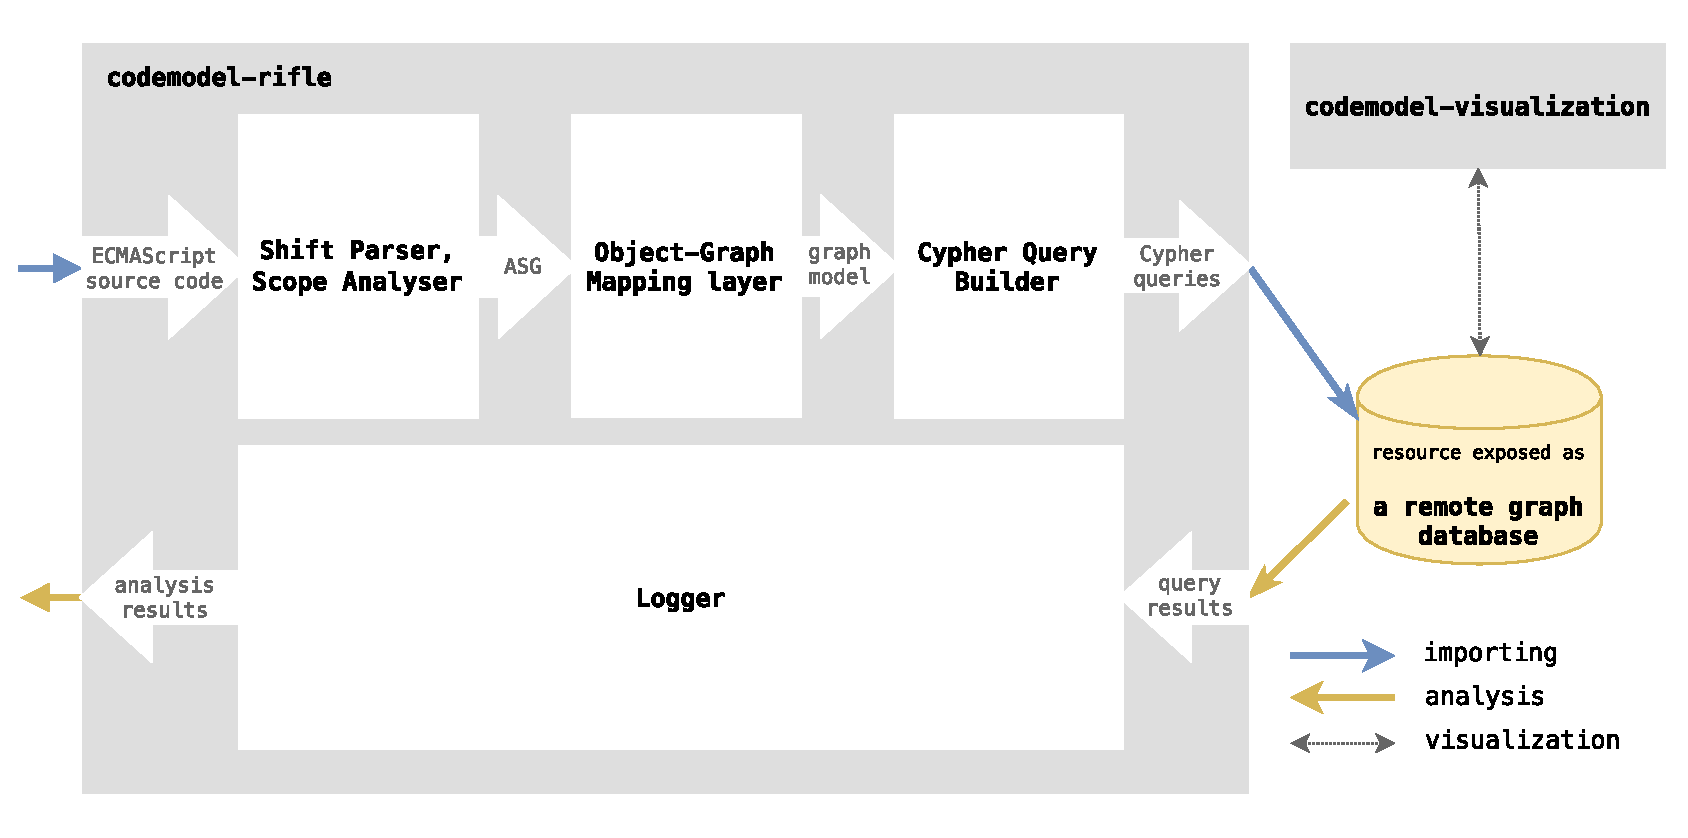
\includegraphics[width=\textwidth, trim=3mm 3mm 3mm 3mm,clip]{figures/codemodel-rifle-refactored-architecture.pdf}
	\caption{The refactored architecture of the Codemodel-Rifle framework}
	\label{fig:codemodel-rifle-refactored-architecture}
\end{figure}


\section{In Development: Steps of Building New Analyses}

Building new analyses to catch new software defects basically consists of three steps. The steps are detailed in the following subsections.


\subsection{Visualising the Defect with Codemodel-Visualisation}

First, the defect has to be inspected with the ASG-semantics of Codemodel-Rifle. For visualising a defect pattern, a new unit test has to be implemented in the Codemodel-Visualization project. The JavaScript module or modules containing the defect should be included as test resources.

Using Codemodel-Rifle as a dependency, Codemodel-Visualization first imports the file (files) and translates it (them) to separate property graphs. If multiple source files are imported, their graphs are connected along the export and import semantics of \es.\footnote{The process of connecting \es modules along export and import statements is one of the key subjects of this thesis. It will be detailed in \Cref{chapter:elaboration}.} Finally, the full property graph model gets exported into a visual file format, like PDF or PNG. The export format is configurable in the unit test itself.


\subsection{Describing the Defect Pattern}

The file exported by Codemodel-Visualization precisely mirrors the property graph instance model translated by Codemodel-Rifle, but some nodes and edges are not displayed to preserve the transparency of the visualised graph.\footnote{Ignored nodes and edges are listed in the \texttt{GraphWalker} class as filtered entities from the underlying visitor pattern implementation.} Any pattern seen in the visualised graph can be directly matched by Codemodel-Rifle.


\subsection{Implementing the Analysis}
\label{subsection:implementing-analyses}

Analyses are basically Cypher queries. If a defect's pattern can be expressed with a Cypher query in some way, it can be detected by the framework.

Some defects are more high-level or more general than to present their patterns in an intact graph directly. Detecting complex errors like these may require to extensively manipulate the graph to dredge defect patterns for matching. In cases involving \emph{transitive} defects, like in the running example\footnote{The running example is to detect a division by zero scenario. But zero is not a numeric literal $0$, but the indirectly referenced return value of a nested function stack with variable assignments and also a module boundary in between.} presented in \Cref{chapter:background}, a flag like \texttt{EqualsZero} has to be propagated through the graph along specified edges: variable assignments, variable references, function call and function return statements, etc.

Transitive graph manipulations can be achieved by introducing \emph{qualifiers} into the analysis. The concept of qualifiers will be described in detail in \Cref{chapter:elaboration}.

If the analysis matches the specified pattern, it returns the following:

\begin{itemize}
\item a \textbf{message} to explain the type of the defect for a human reader,
\item an \textbf{entity name} (or an empty string) to identify defects bound to named entities,
\item the \textbf{path} of the containing module,
\item the \textbf{line} in which the defect was found,
\item the \textbf{column} of the line at which the defect begins.
\end{itemize}

In my current implementation, these items are uniformly\footnote{Exactly these items are returned in all cases, regardless of the defect type.} returned from the database as elements of a Neo4j \texttt{Record}, and they are handed over to a central logger to be immediately printed after minimal formatting. This is not a flexible, extensible solution; in the future, this basic defect processing logic should be refined. The found defects could be returned as JSON objects from the database to be easily parsed into a Java class named \texttt{Defect}. They could also be collected into a per-analysis data structure. This way, the framework could display defects found at an analysis according to various aspects and criteria, and it could also produce machine-readable output for cooperating with other software.


\section{In Production: Steps of Operating Live}

The prospective live operation of the framework basically consists of three steps, which are managed by the framework. Ideally, the operation should be automatic and transparent: if a change is done in the IDE, or a new commit is pushed to the central repository, the framework should perform analyses over the changed code repository. The steps of a full analysis procedure are detailed in the following subsections.


\subsection{Synchronising the Repository into the Framework}

First, the code repository is imported into the framework. This involves listing and parsing all files with configured extensions (currently only \texttt{.js}), then saving the created property graph models into the database.

The word synchronising expresses that Codemodel-Rifle aims to be incremental; but while it does so, its capabilities are still very limited. According to plans, the framework will cooperate with VCSs to detect changes, thus it will be able to import only those files that changed since the last import process.


\subsection{Connecting the Related \es Modules}

To evaluate analyses over multiple \es modules, the related modules' separate property graphs are interconnected along the export and import semantics of \es. This process is described in detail in \Cref{chapter:elaboration}.


\subsection{Performing Analyses}

Performing analyses can be broken down into two substeps.


\subsubsection{Manipulating the Graph}

Complex analyses may require to extensively manipulate the graph. These manipulations involving qualifiers are processed first.


\subsubsection{Querying the Graph}

The graph is queried with Cypher, with matching predefined graph patterns developed with the aforementioned steps. If a defect pattern matches, the defect gets logged onto the console with the semantics described in \Cref{subsection:implementing-analyses}, in the format seen in \Cref{fig:defect-found-logger}.

\vspace{0.5em}
\begin{figure}[!htb]
	\centering
	\texttt{\textbf{message}: \textbf{entityname} at \textbf{line}:\textbf{column} in \textbf{path}}
  \caption{The framework's console output if a defect was found}
  \label{fig:defect-found-logger}
\end{figure}
\chapter{Elaboration of the Workflow}
\label{chapter:elaboration}

This chapter details the implementation of the analyses and the additional proceedings about analysing more than one \es modules coherently. Thus, this chapter encompasses all \emph{semantic} changes of the framework.

Following Dániel Stein~\cite{stein-daniel-msc} and \Cref{chapter:overview} of this thesis, a full analysis procedure of the Codemodel-Rifle framework can be broken down to three distinct phases:

\begin{enumerate}
\item \textsc{\textbf{Import:}} Every \es source file (containing the source code of one \es module) of the analysed code repository is imported into Codemodel-Rifle. The modules are translated to Abstract Semantic Graph models. The ASGs are stored as distinct, per-module property graphs in the underlying Neo4j graph database.
\item \textsc{\textbf{Interconnect:}} The related modules' separate graphs are interconnected along the \emph{export} and \emph{import} semantics of \es. This makes possible to evaluate analyses over more than one modules coherently.
\item \textsc{\textbf{Analyse:}} The predefined analyses are executed.
	\begin{enumerate}
	\item The graph manipulations of the \emph{Qualifier System} are performed.
	\item The defect patterns are matched.
	\end{enumerate}
\end{enumerate}

Since I have not made any semantic changes to the \textsc{Import} phase, this chapter focuses to the \textsc{Interconnect} and the \textsc{Analyse} phases.


\section{Interconnecting Related \es Modules}
\label{section:interconnect}

This section describes the work I made to support analysing more than one \es modules coherently. The approach follows~\cite{stein-daniel-msc}, and completes it by developing the semantics of missing use cases, and then implementing them. To shorty summarise: in order to coherently analyse several related \es modules with the Codemodel-Rifle framework, the related modules' separate property graphs are interconnected by well-defined rules. As previously already mentioned, these rules are built upon the \emph{export} and \emph{import} semantics of \es~\cite{exploringes6}. Equivalently, \es modules are considered to be \emph{related}, if they refer to each other by using \emph{export} and \emph{import} statements.


\subsection{The \es Module System}

As the language gained traction, JavaScript projects rapidly grown to a size where modularisation became critical in order to keep the code logically organised. Today's largest \es code bases include Google's Gmail\footnote{\texttt{https://www.gmail.com}} with approx. 400,000 lines of code~\cite{gmail-loc}, Ruben Daniels' Cloud9 IDE\footnote{\texttt{https://c9.io}} with approx. 300,000 lines of code~\cite{cloud9-loc}, and Lucidchart\footnote{\texttt{https://www.lucidchart.com}} with approx. 200,000 lines of code~\cite{lucidchart-loc}. The product of Tresorit featured in this thesis consists of approx. 35,000 lines of \es code.

Plain JavaScript does not have built-in support for modules~\cite{exploringes6}, there are only community-provided solutions like \emph{RequireJS}\footnote{\texttt{http://requirejs.org}}. In contrary, the 6\textsuperscript{th} version of \es has language-level support for modules: each source file represents exactly one module. Entities like variables and functions defined in one module, or even complete modules themselves can be \emph{exported} to be \emph{imported} to a different module. By default, modules are referred by their relative pathname, without the containing file's extension. Entities that are not explicitly exported remain \emph{private}, meaning they can not be imported to other modules.

In \es 6, there are several ways of exporting and importing entities~\cite{exploringes6}, these are detailed in the next subsections. The Codemodel-Rifle framework had only minimal demonstrative support for interconnecting several \es modules; I extended Dániel Stein's work by covering the most used \emph{export-import case combinations}.


\subsection{Export Syntaxes and Cases}

By default, each entity can only be accessed in the scope of the module it was declared in. To be accessed in other modules, the entity has to be explicitly exported first. \Cref{fig:export-syntaxes} presents export syntax examples of \es 6, based on~\cite{export-syntaxes}. Since these statements can be almost arbitrarily combined, and the number of exported variables is not limited in theory, the list of differing export syntaxes of \es 6 is practically endless.

Therefore, \emph{export syntaxes} need to be distinguished from \emph{export cases}. An \emph{export case} is identified by the \emph{basic form} of an \emph{export syntax}. An \emph{export syntax} written in \emph{basic form} does not combine divers syntaxes, and exports only one entity per export statement. \Cref{fig:export-syntaxes} displays all syntaxes in \emph{basic form}, thus it lists all members of the \emph{distinct export cases'} finite set. Each different \emph{export case} has a unique graph pattern in the ASG.

\begin{figure}[!p]
	\centering
	\begin{lstlisting}[language=JavaScript]
			// exportName
			export { name1, ... };
			// exportDefaultName
			export default name1;
			// exportAlias
			export { name1 as exportedName1, ... };
			// exportAsDefault
			export { name1 as default, ... };
			// exportEmptyLetDeclaration
			export let name1, ... ;
			// exportEmptyVarDeclaration
			export var name1, ... ;
			// exportLetDeclaration
			export let name1 = ..., ... ;
			// exportVarDeclaration
			export var name1 = ..., ... ;
			// exportConstDeclaration
			export const name1 = ..., ... ;
			// exportClass
			export class name1 { ... }
			// exportFunction
			export function name1(...) { ... }
			// exportGenerator
			export function* name1(...) { ... }
			// exportDefaultClass
			export default class name1 { ... }
			// exportDefaultFunction
			export default function name1(...) { ... }
			// exportDefaultGenerator
			export default function* name1(...) { ... }
			// exportDefaultExpression
			export default expression;
			// exportDefaultAnonymousClass
			export default class { ... }
			// exportDefaultAnonymousFunction
			export default function (...) { ... }
			// exportDefaultAnonymousGenerator
			export default function* (...) { ... }
			// exportExpression
			export expression;
			// reexportNamespace
			export * from ...;
			// reexportName
			export { name1, ... } from ... ;
			// reexportAlias
			export { import1 as importedName1, ... } from ...;
	\end{lstlisting}
  \caption{Export syntax examples of \es 6}
  \label{fig:export-syntaxes}
\end{figure}


\subsection{Import Syntaxes and Cases}

An entity declared in module \textbf{A} can be accessed in module \textbf{B}, if \textbf{A} exports, and \textbf{B} imports the entity. All exported entities of a module can be imported as well: in this case an object is created with the name of the imported module's alias, and with members listing the exported entities of the imported module. \Cref{fig:import-syntaxes} present import syntax examples of \es 6, based on~\cite{import-syntaxes}. Like the exports, these statements can also be combined with each other, making the list of the possible import syntax combinations endless.

Thus, \emph{import syntaxes} need to be distinguished from \emph{import cases}, similarly to the exports. An \emph{import case} is identified by the \emph{basic form} of an \emph{import syntax}. \Cref{fig:import-syntaxes} displays all syntaxes in \emph{basic form}. Each different \emph{import case} has a unique graph pattern in the ASG.

\begin{figure}[!htb]
	\begin{lstlisting}[language=JavaScript]
		// importName
		import { name1, ... } from "exporter";
		// importAlias
		import { name1 as importedName1, ... } from "exporter";
		// importDefault
		import defaultName from "exporter";
		// importNamespace
		import * as exportedModule from "exporter";
		// importModule
		import "exporter";
	\end{lstlisting}
  \caption{Import syntax examples of \es 6}
  \label{fig:import-syntaxes}
\end{figure}


\subsection{Number of Export-Import Combinations}

Let $\mathbb{E}$ be set of all the distinct export cases, and let $\mathbb{I}$ be the set of all the distinct import cases. As \Cref{fig:export-syntaxes} and \Cref{fig:import-syntaxes} show, $|\mathbb{E}| = 23$, and $|\mathbb{I}| = 5$. If all export cases would be compatible with all import cases according to the \es grammar, set $\mathbb{C}$ containing all combinations would be $\mathbb{C} = \mathbb{E} \times \mathbb{I}$ with the cardinality of $|\mathbb{C}| = |\mathbb{E}| * |\mathbb{I}| = 23 * 5 = 115$.

\begin{figure}[!htb]
	\begin{lstlisting}[language=JavaScript]
					// exporter.js
					export let name1 = ...;
					// importer.js
					import defaultName from "exporter";
	\end{lstlisting}
  \caption{An example of incompatible export-import cases}
  \label{fig:incompatible-export-import-example}
\end{figure}

Let $\mathbb{S}$ be the set of the export-import combinations supported by Codemodel-Rifle, and let $\alpha$ be the number of distinct algorithms needed to be implemented for supporting every element of $\mathbb{S}$. The following applies: $\alpha \leq |\mathbb{S}|$, since the framework needs one separate algorithm for each export-import case at most. Since not all export cases are compatible with all import cases (a counterexample is displayed on \Cref{fig:incompatible-export-import-example}), the set of \emph{semantically valid} export-import combinations is narrower than $\mathbb{C}$. Codemodel-Rifle should interconnect only semantically valid export-import cases, so $\mathbb{S} \subset \mathbb{C}$. Also, $\alpha$ can be reduced further by involving ASG-specific knowledge: with graph pattern generalisation techniques, several export cases can be handled as one at implementing the interconnections, while preserving semantics. Therefore several export cases can be covered by one algorithm, so $\alpha < |\mathbb{S}|$. In addition, by choosing particular export and import cases not to be supported by Codemodel-Rifle, $\alpha$ can be lowered even further. Case compatibility, unsupported cases and pattern generalisation techniques are detailed in the following subsections.


\subsection{Compatibility of the Export-Import Cases}

An export-import combination is considered to be \emph{semantically valid}, if it complies with the \es grammar~\cite{export-grammar, import-grammar}. Accordingly, semantically valid export-import combinations consist of \emph{compatible} export-import cases: export case \textbf{E} and import case \textbf{I} are considered to be \emph{compatible} with each other, if the entity exported by \textbf{E} can be imported by \textbf{I}, following the \es grammar. \Cref{fig:incompatible-export-import-example} shows an example of incompatible export-import cases. \Cref{table:export-import-compatibility} displays a compatibility matrix for \es export-import cases.

As only semantically valid export-import combinations are required to be supported by Codemodel-Rifle to evaluate analyses over several \es modules coherently, incompatible cases do not need to be covered. This reduces $\alpha$ from $115$ to $84$ (see \Cref{table:export-import-compatibility}).


\subsection{Unsupported Cases}

There are export and import cases which I chosen not be supported by Codemodel-Rifle because of implementation difficulties, or the cases' irrelevant usage. This reduces $\alpha$ from $84$ to $33$. The unsupported export and import cases are the following:

\begin{itemize}
\item \textbf{\lstinline{exportDefaultExpression, exportDefaultAnonymousClass, export\- DefaultAnonymousFunction, exportDefaultAnonymousGenerator}}: There is no clear way for interconnecting the exported entities with the importer module.
\item \textbf{\lstinline{exportExpression}}: Unnamed expressions (e.g.\ \lstinline[language=JavaScript]{export 1 + 2;}) can not be imported, because they can not be referenced.
\item \textbf{\lstinline{reexportName},} \textbf{\lstinline{reexportAlias},} \textbf{\lstinline{reexportNamespace}}: According to my experiences, re-exporting is used very little.
\item \textbf{\lstinline{importNamespace}}: There is no clear solution for including all exported variable of the imported module as an object into the ASG.
\item \textbf{\lstinline{importModule}}: It only loads the module, does not import anything. The first such import in a program executes the body of the module~\cite{exploringes6}.
\end{itemize}

\Cref{table:export-import-compatibility} displays unsupported export and import cases with a grey background. With excluding the incompatible and the unsupported cases from the interconnection process, $\alpha$ is reduced by more than $71\%$, from $115$ to $33$. This saves a significant amount of work without notable loss of the analyses' credibility — unsupported cases were mostly chosen because of their unpopularity. Nevertheless, these cases need to be covered later as well.

\begin{table}[!htb]
	\newcommand{\yep}{\tikz\draw[black,fill=black] (0,0) circle (0.8ex);\xspace}
	\newcommand{\nop}{\tikz\draw[black,fill=none] (0,0) circle (0.8ex);\xspace}

	\definecolor{grey}{gray}{0.85}
	\newcolumntype{g}{>{\columncolor{grey}}c}

	\small
	\centering
	\begin{tabular}{l|cccgg}
		\hline
																				& \rotatebox{90}{importName}
																				& \rotatebox{90}{importAlias}
																				& \rotatebox{90}{importDefault}
																				& \rotatebox{90}{importNamespace~~}
																				& \rotatebox{90}{importModule}
																				\\
		\hline
		{exportName}												& \yep & \yep & \nop & \yep & \yep \\
		{exportDefaultName}									& \yep & \yep & \yep & \yep & \yep \\
		{exportAlias}												& \yep & \yep & \nop & \yep & \yep \\
		{exportAsDefault}										& \nop & \nop & \yep & \nop & \yep \\
		{exportEmptyLetDeclaration}					& \yep & \yep & \nop & \yep & \yep \\
		{exportEmptyVarDeclaration}					& \yep & \yep & \nop & \yep & \yep \\
		{exportLetDeclaration}							& \yep & \yep & \nop & \yep & \yep \\
		{exportVarDeclaration}							& \yep & \yep & \nop & \yep & \yep \\
		{exportConstDeclaration}						& \yep & \yep & \nop & \yep & \yep \\
		{exportClass}												& \yep & \yep & \nop & \yep & \yep \\
		{exportFunction}										& \yep & \yep & \nop & \yep & \yep \\
		{exportGenerator}										& \yep & \yep & \nop & \yep & \yep \\
		{exportDefaultClass}								& \yep & \yep & \yep & \yep & \yep \\
		{exportDefaultFunction}							& \yep & \yep & \yep & \yep & \yep \\
		{exportDefaultGenerator}						& \yep & \yep & \yep & \yep & \yep \\
		\rowcolor{grey}
		{exportDefaultExpression}						& \nop & \nop & \yep & \nop & \yep \\
		\rowcolor{grey}
		{exportDefaultAnonymousClass}				& \nop & \nop & \yep & \nop & \yep \\
		\rowcolor{grey}
		{exportDefaultAnonymousFunction}		& \nop & \nop & \yep & \nop & \yep \\
		\rowcolor{grey}
		{exportDefaultAnonymousGenerator}		& \nop & \nop & \yep & \nop & \yep \\
		\rowcolor{grey}
		{exportExpression}									& \nop & \nop & \nop & \nop & \yep \\
		\rowcolor{grey}
		{reexportName}											& \yep & \yep & \nop & \yep & \yep \\
		\rowcolor{grey}
		{reexportAlias}											& \yep & \yep & \nop & \yep & \yep \\
		\rowcolor{grey}
		{reexportNamespace}									& \yep & \yep & \yep & \yep & \yep \\
		\hline
	\end{tabular}

	\caption{Export-import compatibility matrix with unsupported cases in grey}
	\label{table:export-import-compatibility}
\end{table}


\subsection{Pattern Generalisation Techniques}

After excluding the incompatible and the unsupported cases, $33$ different import-export combinations still need to be covered by the interconnection process. This would imply that $\alpha = 33$ algorithms are needed for all combinations, but $\alpha$ can be reduced further by involving ASG-specific knowledge. At interconnecting modules, several export cases' graph patterns can be matched by one, somehow generalised pattern description, and thus several export cases can be interconnected with the same algorithm. For import cases, generalisation is neither possible nor necessary, since only three, semantically different import cases are supported by Codemodel-Rifle. To proceed, two concepts are defined.

\paragraph{Semantically correct interconnection}

An export-import interconnection between two modules' property graphs is \emph{semantically correct} to Codemodel-Rifle, if the interconnection is reversible, it correlates with the semantics of \es, and the interconnected property graphs contain the same information as the separate property graphs.

\paragraph{Isomorphic export case}

Two export cases are \emph{isomorphic}, if they contain ASG patterns which can be interconnected to an import case along the same nodes and edges, applying the same algorithm, and the interconnection is semantically correct.

Applying the two definitions, my workflow was the following for finding the isomorphic export cases in order to reduce $\alpha$:

\begin{enumerate}
\item I inspected the similarly looking export cases' ASG patterns, whether they can be described by one, somehow generalised graph pattern description.
\item If yes, I examined if the two export cases can be interconnected with import cases along the same nodes and edges, with the same algorithm.
\item If yes, I performed the interconnections, and inspected them whether they are semantically correct.
\item If yes, the two export cases are isomorphic.
\end{enumerate}

\Cref{fig:export-declaration-demonstration} presents two distinct ASGs of two isomorphic export cases as an example. These two cases are described below with also specifying their location on the figure:
\begin{itemize}
\item \textsc{on the left:}\enskip\lstinline[language=JavaScript]{export let name1 = "name1Value"}
\item \textsc{on the right:}\enskip\lstinline[language=JavaScript]{export function name1()}\texttt{ \{ }\lstinline{return "name1Value";}\texttt{ \}}
\end{itemize}

The two export cases are isomorphic because of the following.
\begin{enumerate}[label=\alph*)]
\item \emph{The two graphs contain patterns which can be matched by one pattern description.} Even though these patterns (indicated with thicker outlines) contain nodes and edges with different labels and properties, in Neo4j it is possible to match both of them with only one Cypher expression.
\item \emph{Both patterns can be interconnected to an import along the same nodes and edges applying the same algorithm.} Applying the semantics of Codemodel-Rifle developed along practical reasons, only the node labeled as \lstinline{Declaration} (indicated with blue filling) needs to be connected to the import module's ASG in both cases.
\item \emph{The interconnection is semantically correct.} In both cases, the interconnection is reversible, and no information is lost. The interconnection also correlates with the semantics of \es: in both cases, it expresses that a \emph{named declaration} has been imported from another module. For the aim of the Codemodel-Rifle framework — which is revealing possible errors in software by static analysis — this is a satisfactory way of implementing the interconnections.
\end{enumerate}

\begin{figure}[!htb]
	\centerfloat
	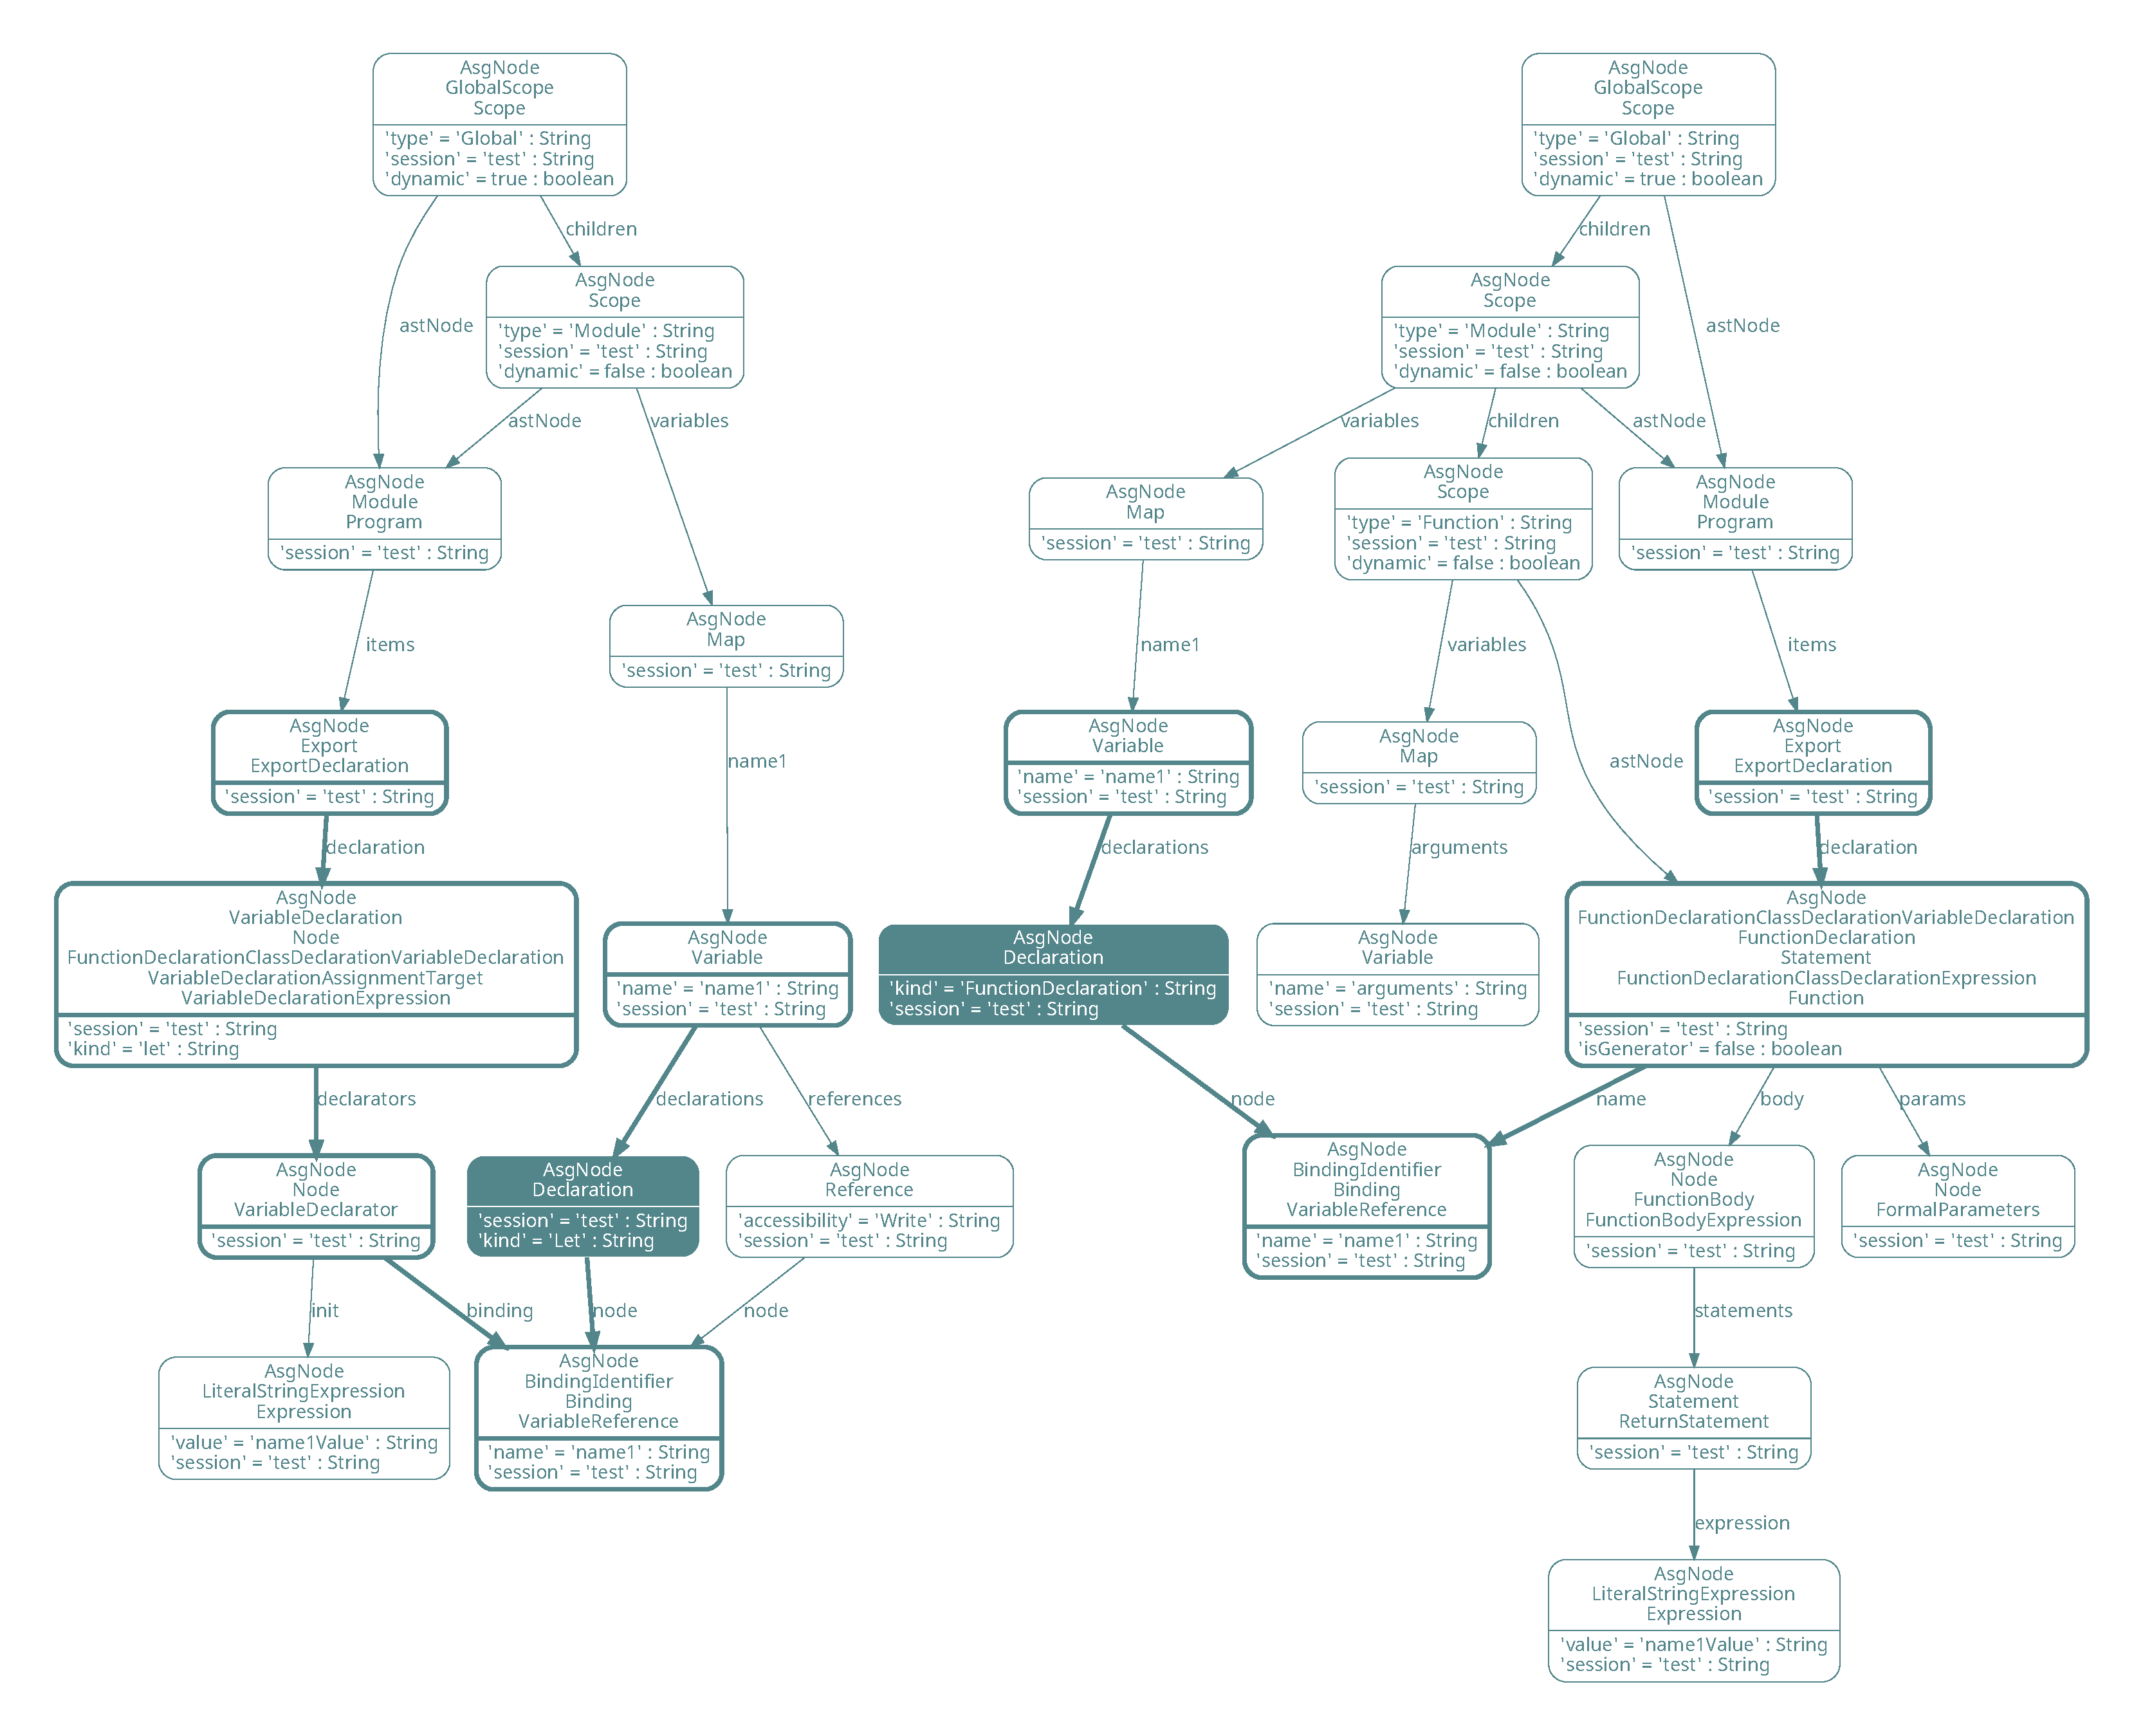
\includegraphics[width=\textwidth+3cm, trim=12mm 12mm 12mm 12mm,clip]{figures/export-declaration-demonstration.pdf}
	\caption{Two isomorphic export cases contain the same pattern}
	\label{fig:export-declaration-demonstration}
\end{figure}

The process of pattern generalisation needs to be performed carefully. The generalised patterns must match only those export cases' patterns that can be interconnected with imports in a semantically correct way. If the patterns are too broadly generalised, they will match more export cases than intended, resulting semantically incorrect interconnections (between incompatible export-import cases). In contrary, if they are too narrowly specified, they will match only one export case, resulting no reduction of the $\alpha$.

In the following, I list all export cases I found to be isomorphic in groups. Each group's name implies why the elements are isomorphic in the group. Since every element can be interconnected with imports using the same algorithm per group, an isomorphic group with its elements can be considered as one generalised export case regarding the ASG interconnection process of the Codemodel-Rifle framework. The following $5$ isomorphic export groups have been formed:

\begin{itemize}
\item \textbf{\lstinline{exportName}}
	\begin{itemize}
	\item \lstinline{exportName}
	\end{itemize}

\item \textbf{\lstinline{exportDefaultName}}
	\begin{itemize}
	\item \lstinline{exportDefaultName}
	\end{itemize}

\item \textbf{\lstinline{exportAlias}}
	\begin{itemize}
	\item \lstinline{exportAlias}
	\item \lstinline{exportAsDefault}
	\end{itemize}

\item \textbf{\lstinline{exportDeclaration}}
	\begin{itemize}
	\item \lstinline{exportEmptyLetDeclaration}
	\item \lstinline{exportEmptyVarDeclaration}
	\item \lstinline{exportLetDeclaration}
	\item \lstinline{exportVarDeclaration}
	\item \lstinline{exportConstDeclaration}
	\item \lstinline{exportClass}
	\item \lstinline{exportFunction}
	\item \lstinline{exportGenerator}
	\end{itemize}

\item \textbf{\lstinline{exportDefaultDeclaration}}
	\begin{itemize}
	\item \lstinline{exportDefaultClass}
	\item \lstinline{exportDefaultFunction}
	\item \lstinline{exportDefaultGenerator}
	\end{itemize}
\end{itemize}

Based on the above, having $5$ isomorphic export groups means that the number of distinctly handled export cases has been reduced to $5$. \Cref{table:updated-compatibility-table} shows the updated compatibility table with export cases grouped by their isomorphism, without listing the unsupported cases. By this time, with excluding incompatible and unsupported cases and applying pattern generalisation techniques, $\alpha$ has been reduced to $13$, meaning only $13$ separate algorithms have to be implemented in order to cover most of the export-import cases.

\begin{table}[!htb]
	\newcommand{\yep}{\tikz\draw[black,fill=black] (0,0) circle (0.8ex);\xspace}
	\newcommand{\nop}{\tikz\draw[black,fill=none] (0,0) circle (0.8ex);\xspace}

	\centering
	\small
	\begin{tabular}{l|ccc}
		\hline
																& \rotatebox{90}{importName}
																& \rotatebox{90}{importAlias}
																& \rotatebox{90}{importDefault~~}
																\\
		\hline
		exportName									& \yep & \yep & \nop \\
		exportDefaultName						& \yep & \yep & \yep \\
		exportAlias									& \yep & \yep & \yep \\
		exportDeclaration						& \yep & \yep & \nop \\
		exportDefaultDeclaration		& \yep & \yep & \yep \\
		\hline
	\end{tabular}

	\caption{Export-import compatibility matrix with exports grouped by their isomorphism}
	\label{table:updated-compatibility-table}
\end{table}


\subsection{Implementing the Interconnection Algorithms}

After thoroughly inspecting the ASG signatures of the numerous export and import cases for minimising the number of algorithms to be implemented, actually implementing the algorithms was straightforward. In this section, I will not present all combinations in detail. Instead, I describe the general steps of the interconnection process, and I provide a complete example with one concrete combination. In the Appendix, all export-import case combinations are listed with their interconnection algorithms.

The steps of the interconnection process in general can be described as follows:

\begin{enumerate}
\item Match each to-be-exported entities of the exporter module with strictly unique patterns containing all necessary identifiers and information for the export.
\item Match each to-be-imported entities of the importer module with strictly unique patterns containing all necessary identifiers and information for the import.
\item Perform interconnections between the exporter module and the importer module by finding corresponding entities in the two modules based on identifiers like names and/or default export/import bindings.
\item Clean the graph, so it will not contain duplicate nodes or edges after the interconnection process.
\end{enumerate}

\vspace*{-3mm}
\begin{figure}[!htb]
	\begin{lstlisting}[language=JavaScript]
			// exporter.js
			let name1 = "name1Value";
			export { name1 };

			// importer.js
			import { name1 as importedName1 } from "exporter";
	\end{lstlisting}
  \caption{Modules for demonstrating the \emph{exportName–importAlias} combination}
  \label{fig:export-import-example-source}
\end{figure}

I chose the fully detailed combination to be the \emph{exportName–importAlias}. The \emph{exportName} case is in the \lstinline{exporter} module, the \emph{importAlias} case is in the \lstinline{importer} module. \Cref{fig:export-import-example-source} shows the source code of the two modules.

\Cref{fig:export-import-example-asg} displays the process of interconnecting the \lstinline{exporter} module's graph with the \lstinline{importer} module's graph along the \emph{exportName–importAlias} case combination. The following steps are performed on the ASGs of the modules:
\begin{enumerate}
\item Find the exported \lstinline{Variable} with its \lstinline{Declaration} in the \lstinline{exporter} module marked with blue colour. The full matched pattern is indicated with thicker outlines.
\item Find the imported \lstinline{Variable} with its \lstinline{BindingIdentifier} and its \lstinline{Declaration} in the \lstinline{importer} module marked with crimson colour. The full matched pattern is indicated with thicker outlines.
\item Check if the \lstinline{Import} node's \lstinline{moduleSpecifier} attribute is equal to the exporter module's name, which is currently \lstinline{exporter}.
\item Check if the \lstinline{name} attribute of the \lstinline{IdentifierExpression} node (connecting to the \lstinline{ExportLocalSpecifier} node) is equal to the \lstinline{ImportSpecifier} node's \lstinline{name} attribute. In this particular \emph{importAlias} case, checking \lstinline{ImportSpecifier} node's \lstinline{name} attribute instead of the imported \lstinline{Variable} node's \lstinline{name} attribute provides the support for the \emph{aliased} import.
\item Create a \lstinline{declarations} edge from the imported \lstinline{Variable} node to the exported \lstinline{Declaration}. This is indicated with a thick black outline.
\item Create a \lstinline{node} edge from the exported \lstinline{Declaration} node to the imported variable's \lstinline{BindingIdentifier} node. This is indicated with a thick black outline.
\item Delete the original \lstinline{Declaration} node of the imported variable with its edges.\footnote{This step does not cause loss of information: the graph still contains the information that the variable was \emph{imported}.} These are indicated with dashed outlines.
\end{enumerate}

These steps are translated to Cypher, and sent to the database. Each export-import combination featured in \Cref{table:updated-compatibility-table} has a separate Cypher query. As these \emph{export-import interconnection queries} are \emph{independent} from each other — they do not modify the others' results in any way — they can be executed in any order. The queries are also \emph{idempotent}: they can be re-executed arbitrarily many times without different outcomes on the same dataset.

\Cref{fig:export-import-example-cypher-source} presents the full Cypher query of the \emph{exportName–importAlias} combination. The query contains a node with a label that is not displayed in the visualised graph: \lstinline{CompilationUnit}. At translating the modules into ASGs, Codemodel-Rifle creates a node with the label \lstinline{CompilationUnit} for each distinct source file. Each module's all graph nodes are connected to the module's \lstinline{CompilationUnit} node. The node also stores information about the parsed module's file path. As displaying the \lstinline{CompilationUnit} nodes with all their connections would make the graph very dense, they are omitted.

\newpage
\vspace*{5em}
\begin{figure}[!h]
	\centerfloat
	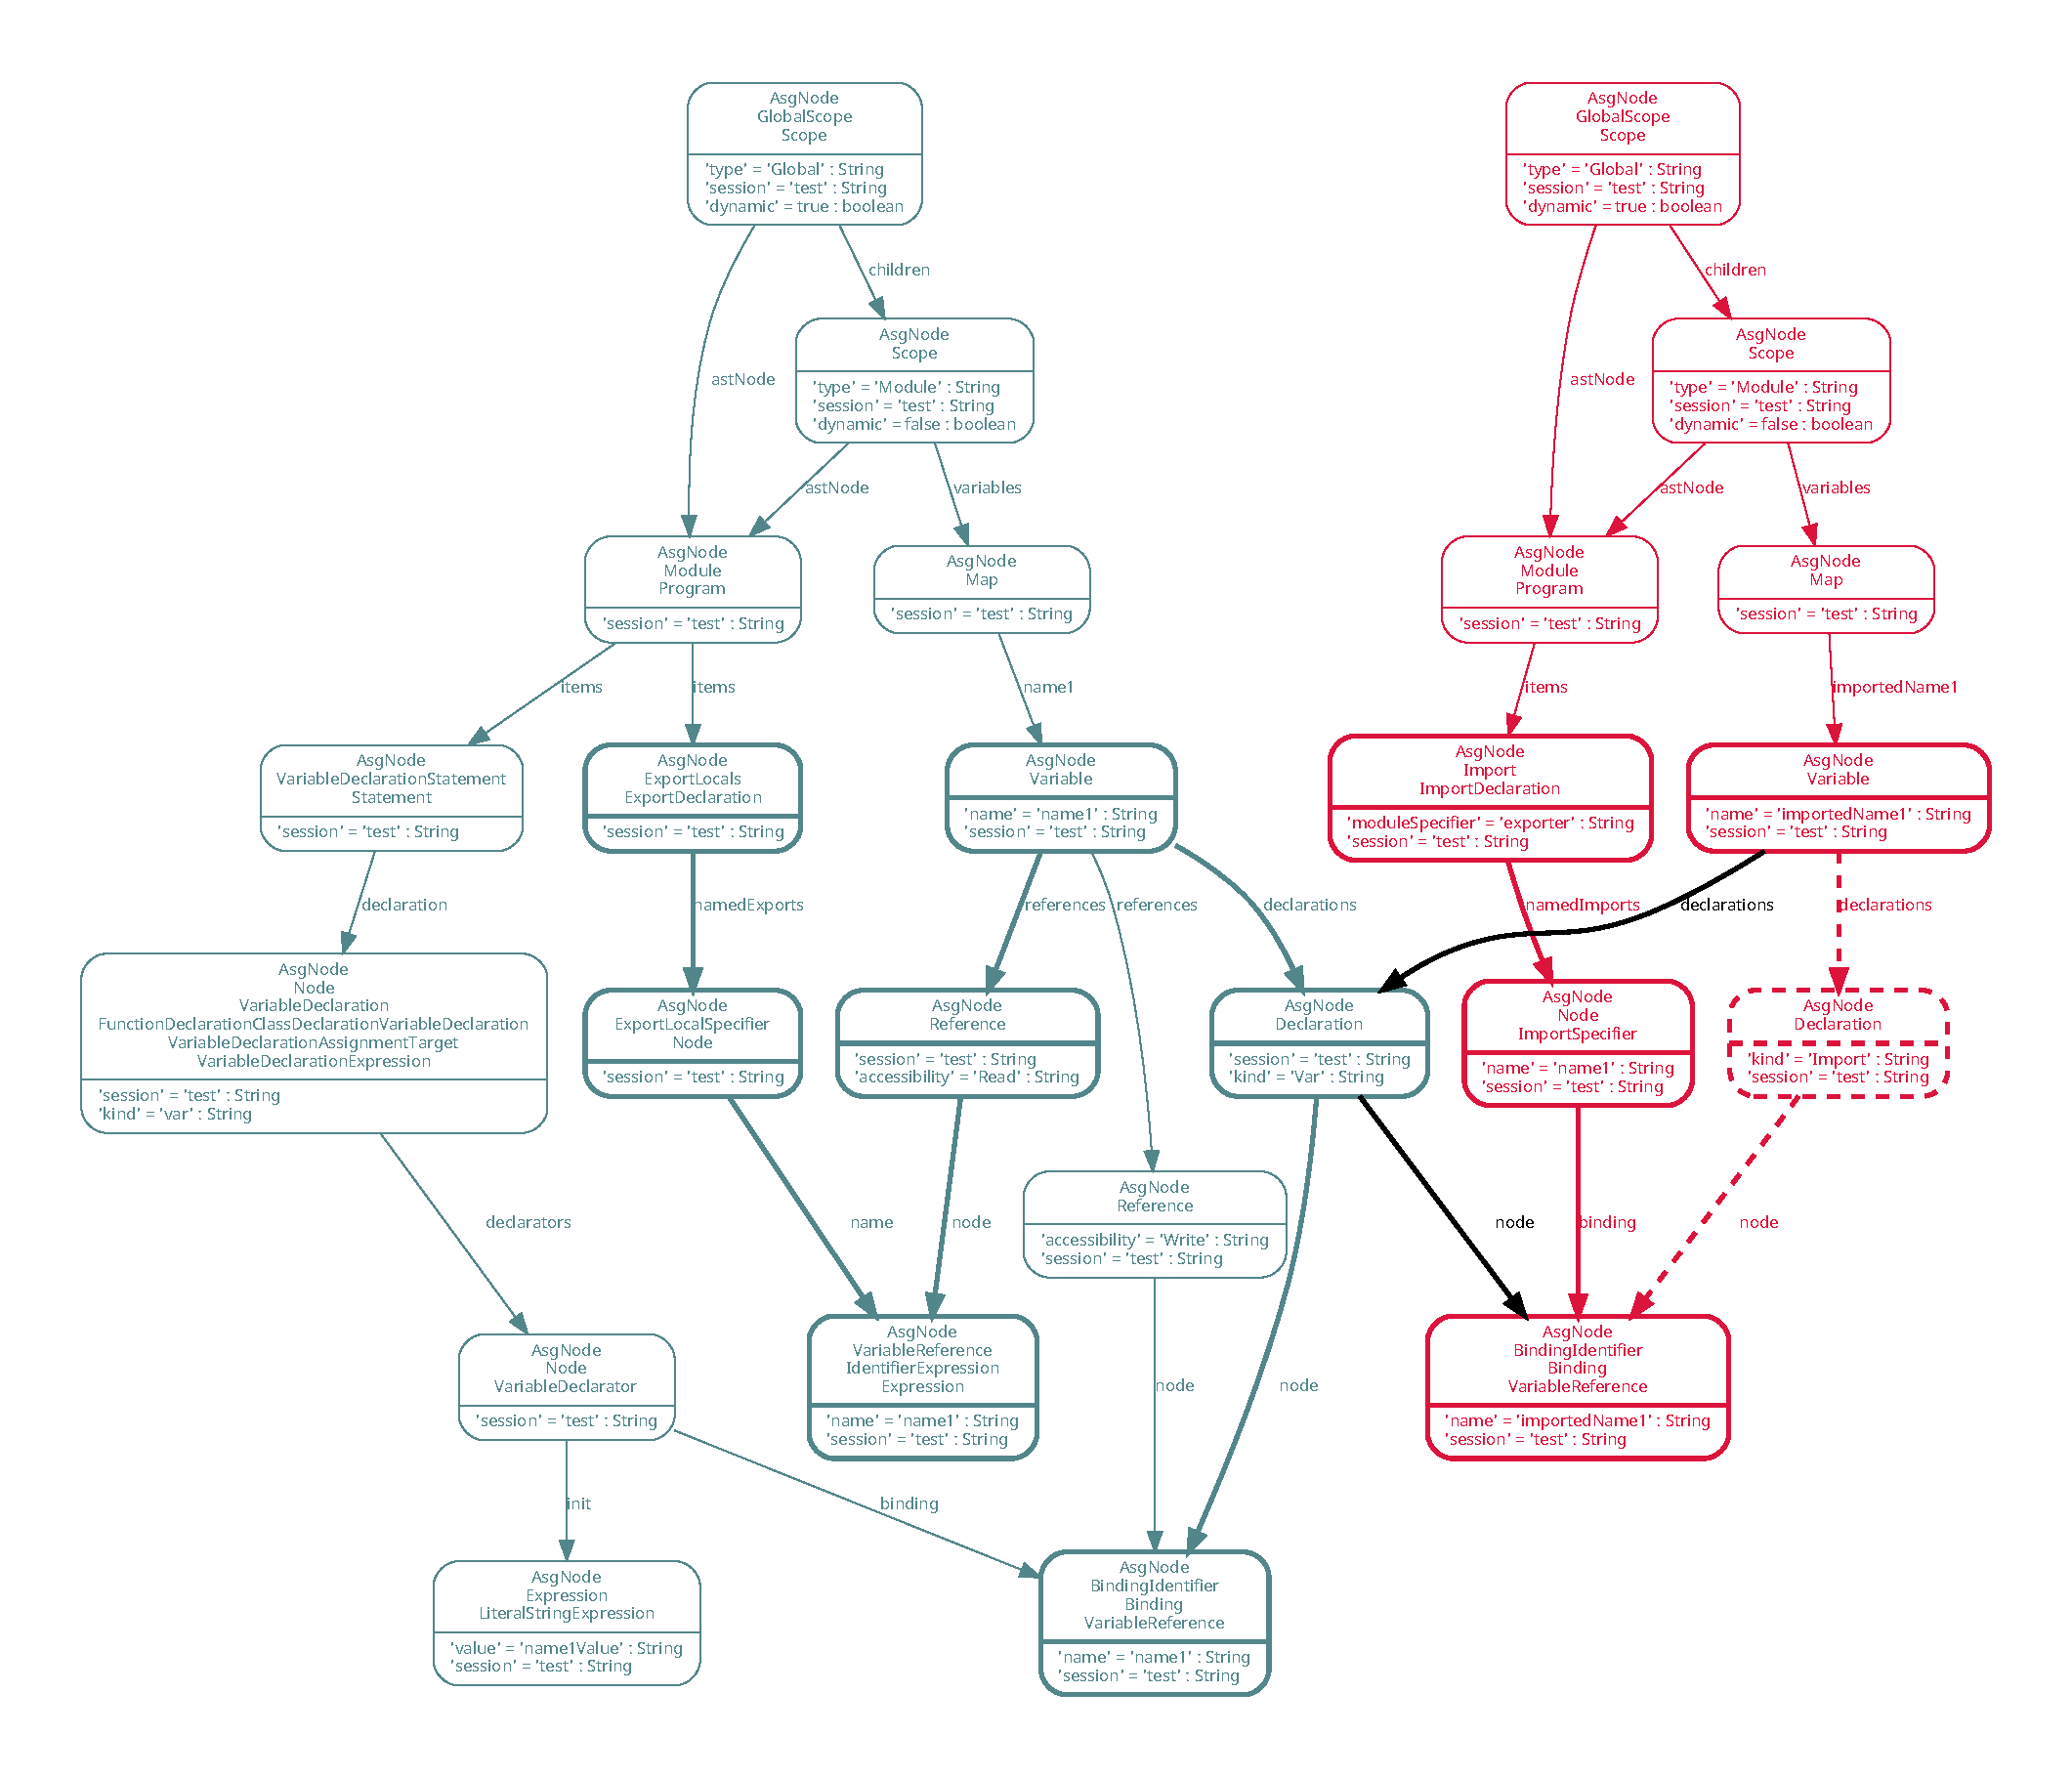
\includegraphics[width=\textwidth+4cm, trim=12mm 12mm 12mm 12mm,clip]{figures/export-import-example-asg.pdf}
	\caption{Interconnecting the \lstinline{exporter} module with the \lstinline{importer} module in the export-import combination \emph{exportName–importAlias}}
	\label{fig:export-import-example-asg}
\end{figure}

\newpage
\vspace*{8.35em}
\begin{figure}[!h]
	\begin{lstlisting}[language=Cypher]
MATCH
// exporter.js: let name1 = "name1Value"; export { name1 };
    (exporter:CompilationUnit)-[:contains]->(:ExportLocals)
        -[:namedExports]->(:ExportLocalSpecifier)
        -[:name]->(exportBindingIdentifier:IdentifierExpression)
        <-[:node]-(:Reference)
        <-[:references]-(:Variable)
        -[:declarations]->(declarationToMerge:Declaration)
        -[:node]->(:BindingIdentifier),

// importer.js: import { name1 as importedName1 } from "exporter";
    (importer:CompilationUnit)-[:contains]->(import:Import)
        -[:namedImports]->(importSpecifier:ImportSpecifier)
        -[:binding]->(importBindingIdentifierToMerge:BindingIdentifier)
        <-[:node]-(declarationToDelete:Declaration)
        <-[:declarations]-(importedVariable:Variable)

    WHERE
    exporter.parsedFilePath CONTAINS import.moduleSpecifier
    AND exportBindingIdentifier.name = importSpecifier.name

MERGE
    (importedVariable)-[:declarations]->(declarationToMerge)
        -[:node]->(importBindingIdentifierToMerge)

DETACH DELETE
    declarationToDelete
	\end{lstlisting}
  \caption{The Cypher query interconnecting the \emph{exportName–importAlias} combination}
  \label{fig:export-import-example-cypher-source}
\end{figure}


\newpage
\section{Simple Analyses by Pattern Matching}

In the Codemodel-Rifle framework, analyses are basically Cypher queries. If a defect's pattern in the Abstract Semantic Graph can be expressed with a Cypher query, it can be detected by the framework. This section details those analyses I implemented for Codemodel-Rifle, which use only pattern matching and do not require to alter the graph.

I developed the analyses by the process I presented in \Cref{section:steps-of-building-new-analyses}. After visualising the defect's pattern with Codemodel-Visualisation, I created the description of the defect by implementing a Cypher query for matching its pattern in the ASG model. The results of the analyses are returned as strings containing defect properties, as described in \Cref{subsection:implementing-analyses}.


\subsection{Uninitialised Variables}

A variable is uninitialised if it was declared but given no value. In most programming languages, uninitialised variables do have \emph{some} value, but it is usually unpredictable \emph{memory garbage} originating from prior values stored at the variable's memory location.

Contrarily in JavaScript, uninitialised variables do not contain random memory garbage. A method or statement evaluating a variable that has not been assigned a value returns \lstinline{undefined}; a primitive value and also a primitive type of JavaScript. Uninitialised variables are of type \lstinline{undefined} with the value \lstinline{undefined}. Per se, uninitialised variables are not defects, but if an uninitialised variable is used without checking whether it is \lstinline{undefined}, it can break code execution in several ways: e.g.\ making the result of the evaluating expression \lstinline{undefined} too, or throwing a \lstinline{ReferenceError}.

\begin{figure}[!htb]
	\centering
	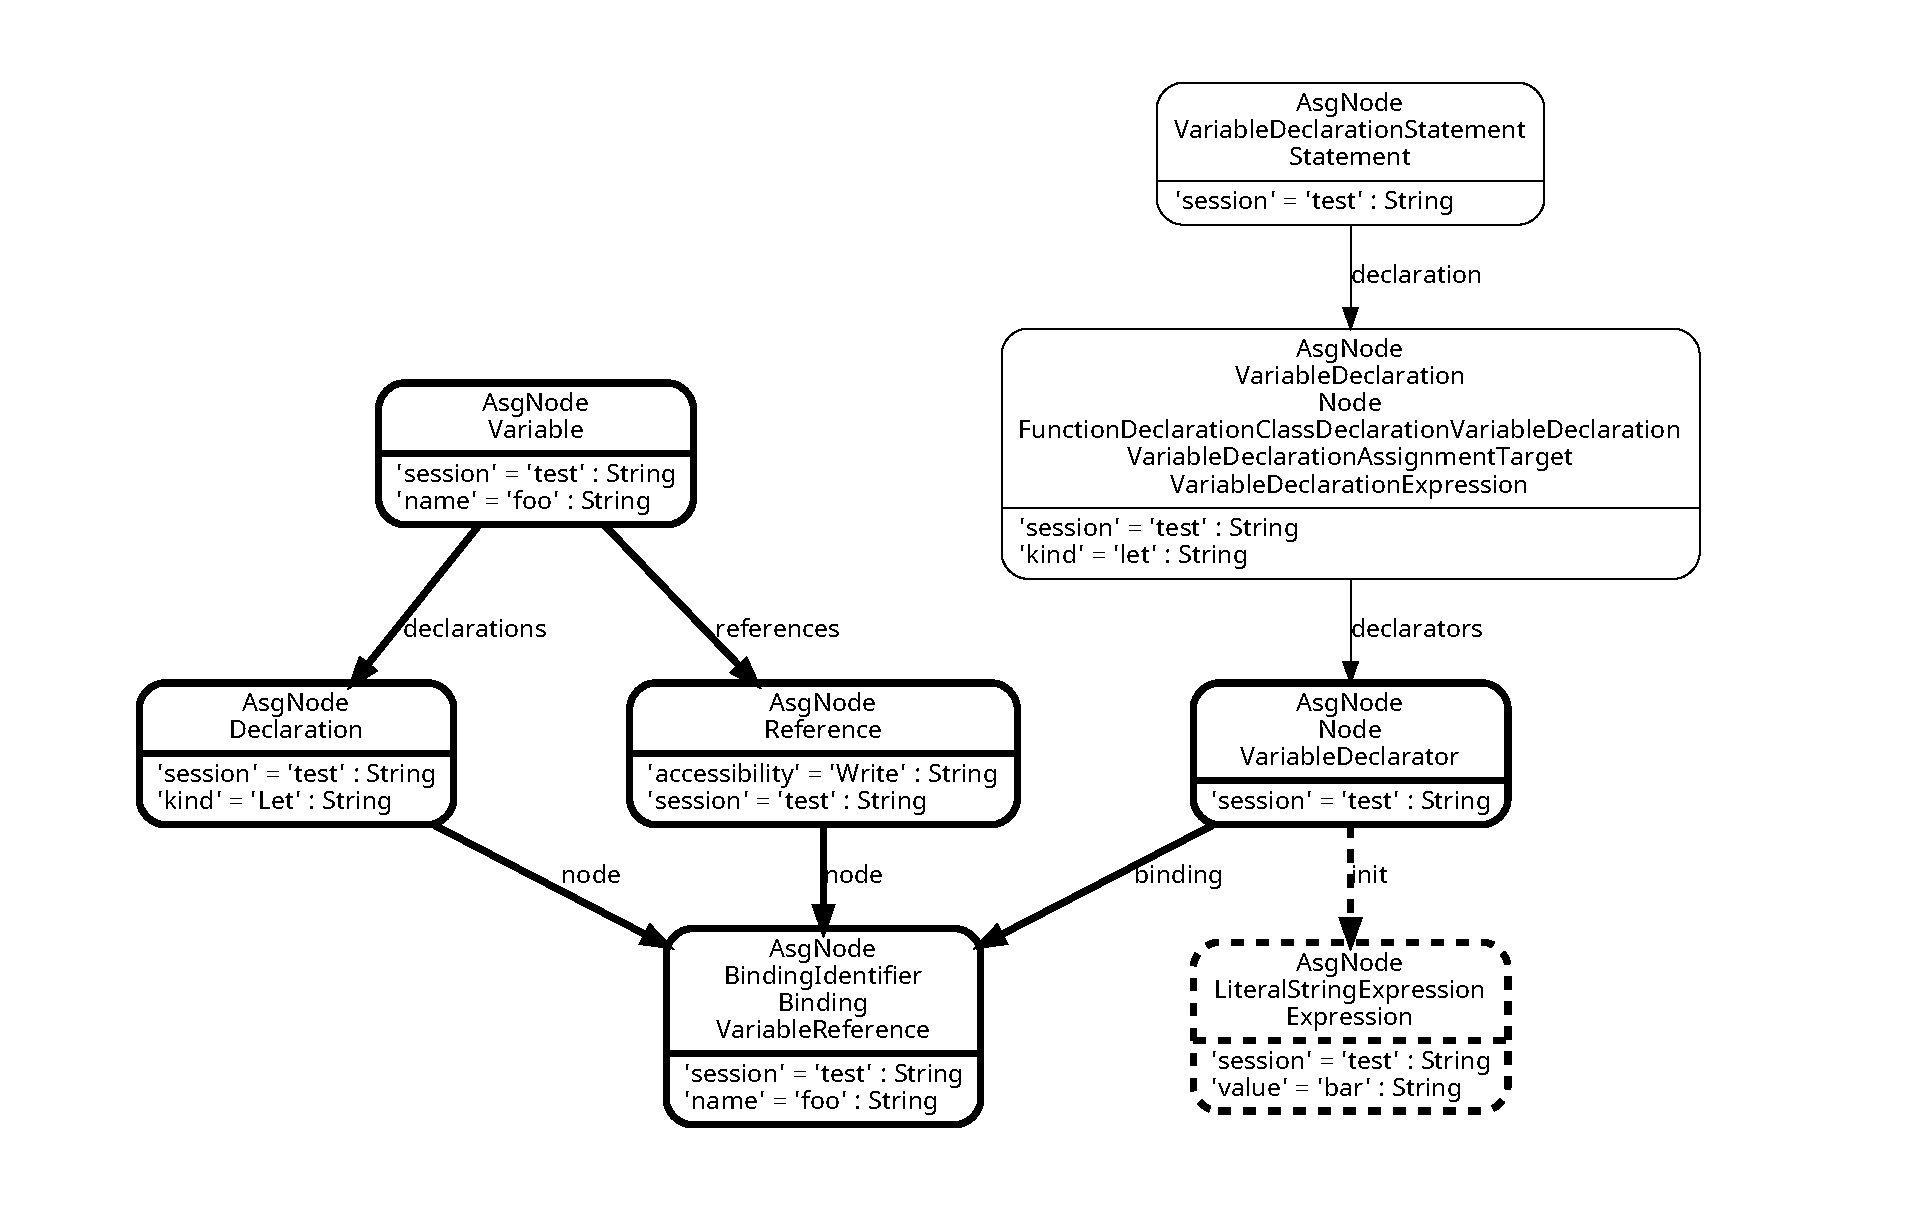
\includegraphics[height=69mm, trim=12mm 12mm 12mm 12mm,clip]{figures/analysis_nonInitializedVariable.pdf}
	\caption{Matching the \lstinline{nonInitialisedVariable} analysis pattern}
	\label{fig:analysis-noninitialisedvariable}
\end{figure}

Regarding uninitialised variables, my analysis in Codemodel-Rifle reports if a variable was not explicitly initialised with an assignment expression.\footnote{The analysis only covers unconditional cases, reporting results of conditional value assignments is currently not supported.} ASG-semantically, this means verifying that the variable's \lstinline{VariableDeclarator} node has no \lstinline{init} relationship. \Cref{fig:analysis-noninitialisedvariable} presents a partial ASG demonstrating how an uninitialised variable is revealed. The nodes with thicker outlines are members of the pattern matching expression, the dashed outlines represent entities being checked for existence. The source code of the analysis is available in the Appendix.


\subsection{Globally Unused Exports}

The \es module system provides a practical solution for keeping code bases organised: logically separated, but practically cooperating software components can be implemented. Exporting only particular entities from a module allows to hide several sensitive information from the outside, such as internal functioning and implementation details, or even security-related specialities. Thus, a best practice is to only export what is explicitly intended to be public, and keep everything else private.

Unused exports can be a security concern. My analysis for detecting unused exports report if an entity is exported, but never imported to any other module. It is based on the semantics of the module interconnections described in \Cref{section:interconnect}.

\Cref{fig:analysis-unusedexport} presents a partial ASG demonstrating how an unused export is revealed. Nodes of the exporter module's graph are indicated with blue colour, nodes of the importer module's graph are indicated with crimson colour. The nodes with thicker outlines are members of the pattern matching expression, the dashed outlines represent entities being checked for existence. The source code of the analysis is available in the Appendix.

\vspace*{1mm}
\begin{figure}[!htb]
	\centering
	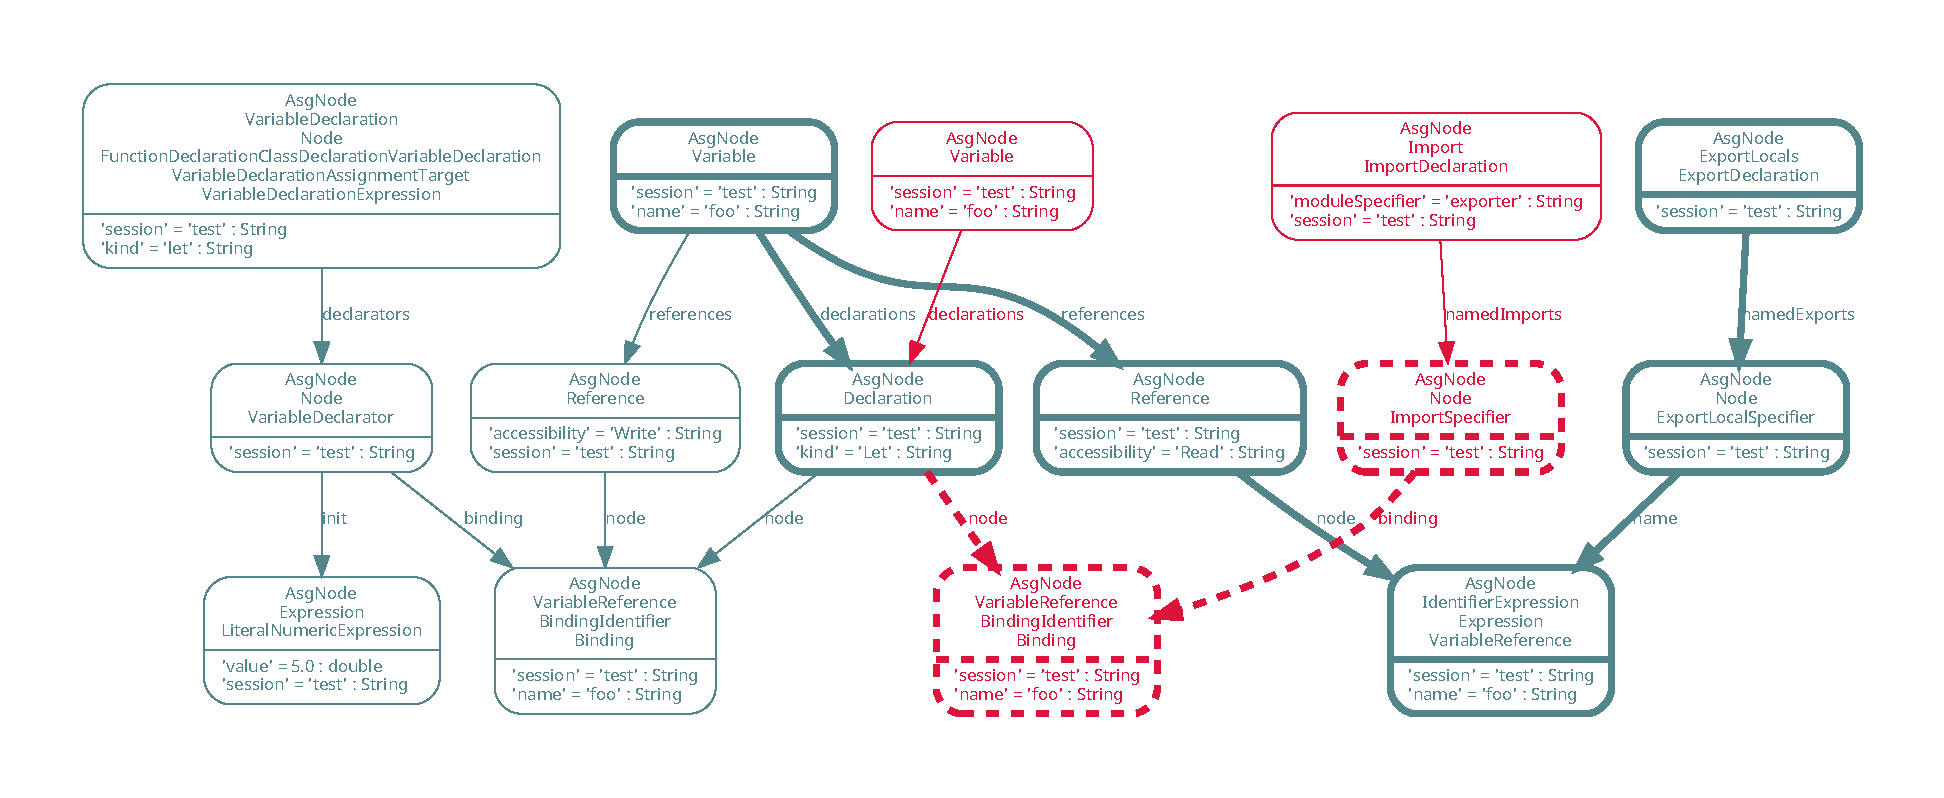
\includegraphics[width=\textwidth, trim=12mm 12mm 12mm 12mm,clip]{figures/analysis_exportName.pdf}
	\caption{Matching the \lstinline{unusedExport_exportName} analysis pattern}
	\label{fig:analysis-unusedexport}
\end{figure}


\subsection{Division By Zero (restricted)}

Division by zero is one of the most basic software defects. JavaScript usually does not throw an error if it evaluates such expressions, but returns \lstinline{undefined}, \lstinline{NaN} or \lstinline{Infinity} instead, depending on the environment and the runtime. As stated before, this can break program execution in several ways.

Detecting a division by zero scenario generally is rather challenging by using only static tools. As the right-hand operator of a division expression can be a variable, whose value can be anything — even originate from several other variables —, it needs much more effort than simple pattern matching. Detecting such \emph{transitive} division by zero cases is the subject of the next section, involving the Qualifier System.

However, finding division expressions in the ASG, where the right-hand operator is a numeric literal with the value zero is not complicated. My analysis for this \emph{restricted} case reports such division by zero defects by simple graph pattern matching.

\Cref{fig:analysis-divisionbyzero-simple} presents a partial ASG demonstrating how a division by zero defect is revealed when zero is a numeric literal. The nodes with thicker outlines are members of the pattern matching expression, and the \lstinline{`value'} property of the \lstinline{LiteralNumericExpression} is checked if it equals zero.

\begin{figure}[!htb]
	\centering
	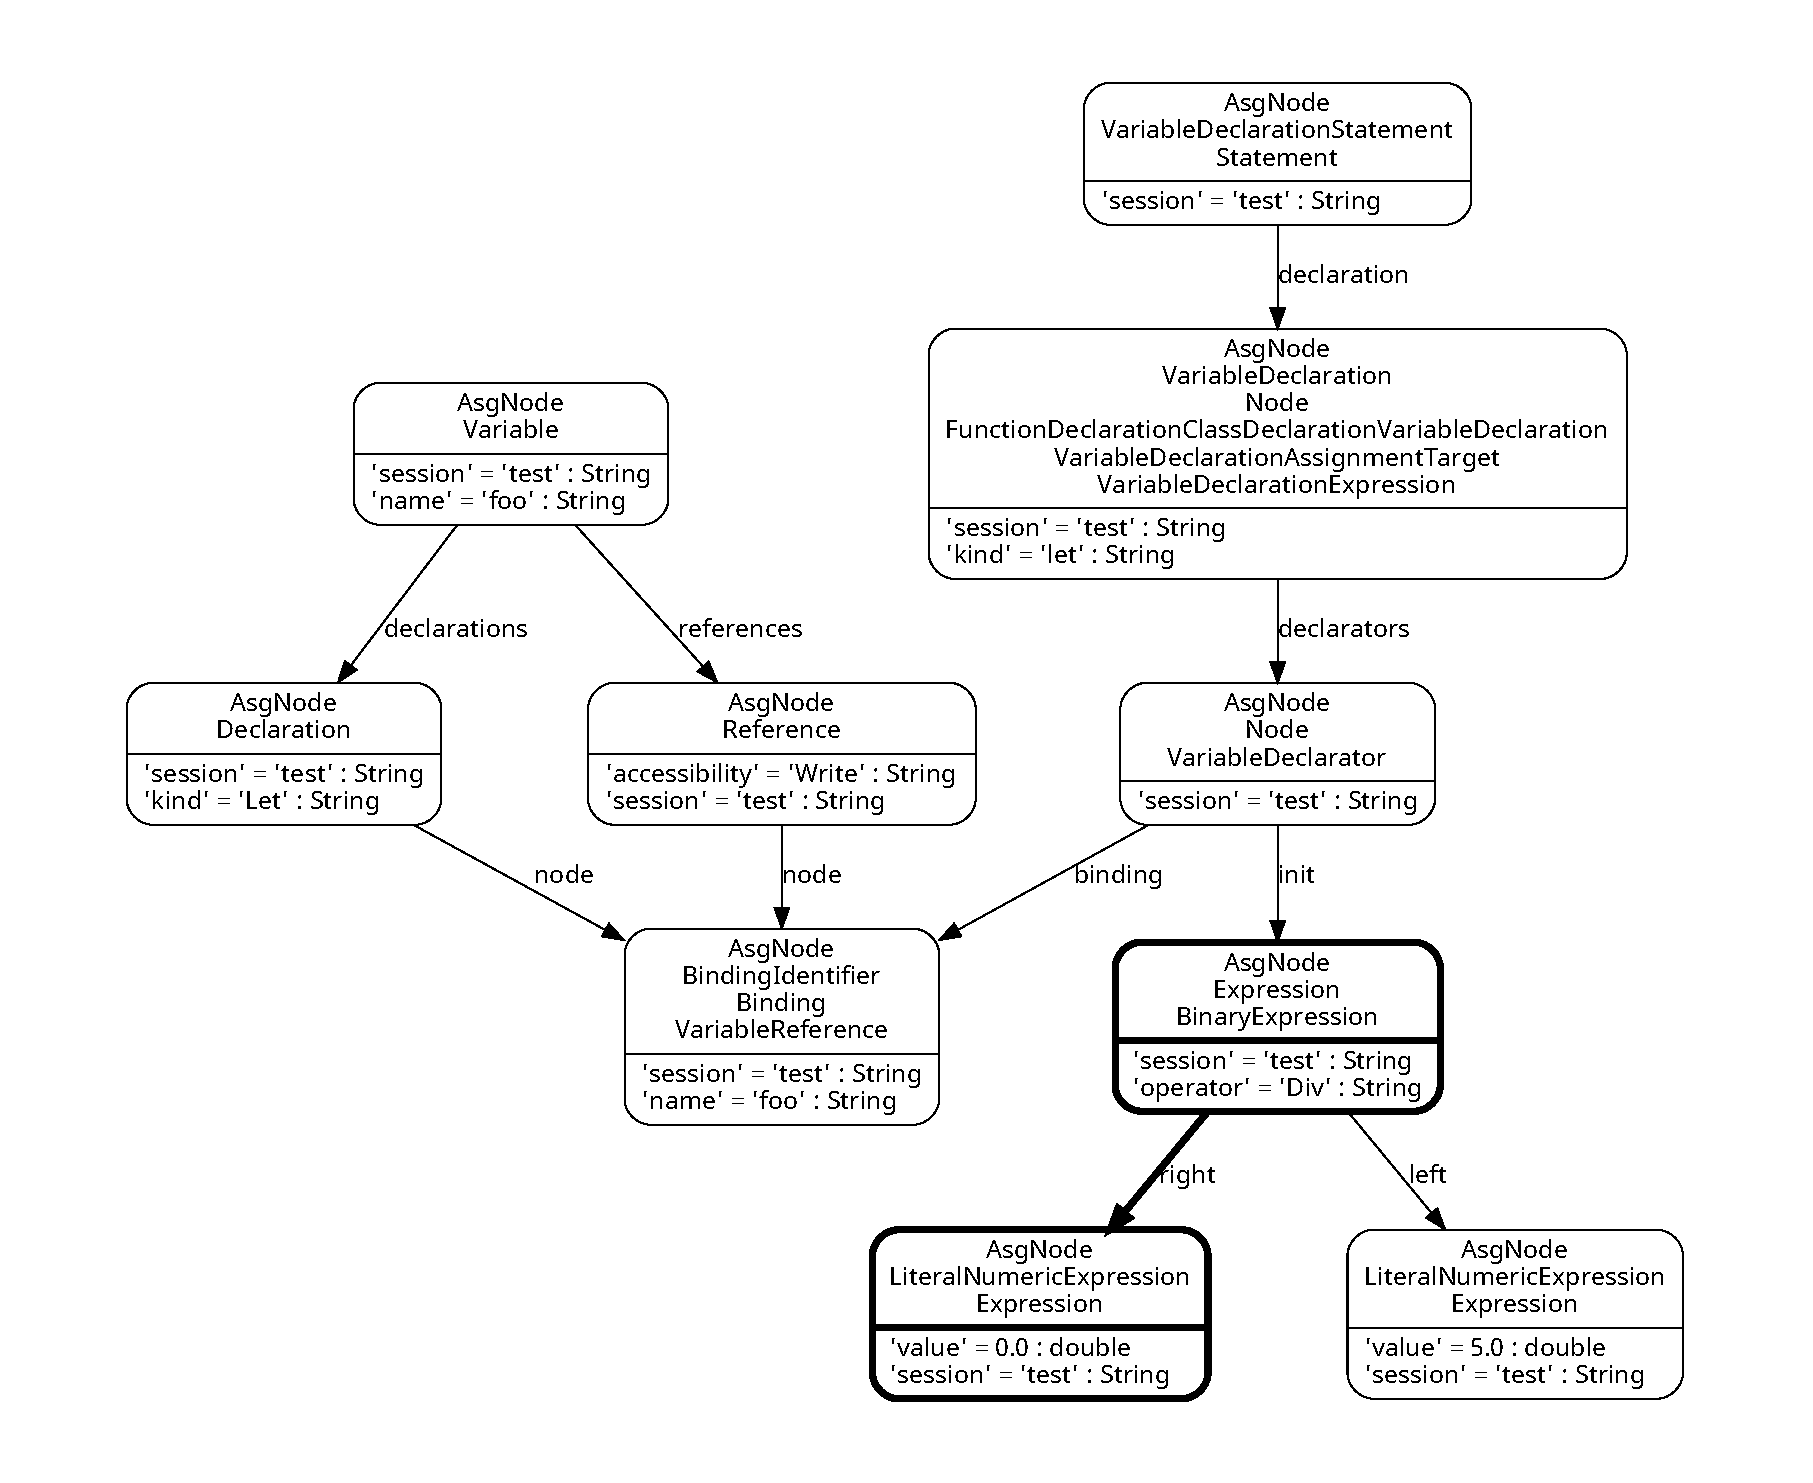
\includegraphics[height=91mm, trim=12mm 12mm 12mm 12mm,clip]{figures/analysis_divisionByZero_simple.pdf}
	\caption{Matching the \lstinline{divisionByZero-literal} analysis pattern}
	\label{fig:analysis-divisionbyzero-simple}
\end{figure}


\subsection{Misuse of Negative Integers as Function Arguments (restricted)}

Generally used functions in JavaScript's \lstinline{Math} library do not support complex numbers. Therefore, if a developer supplies a negative numeric value to a function like \lstinline{Math.sqrt()} or \lstinline{Math.log()}, the expression will return \lstinline{NaN} or \lstinline{undefined}, depending on the environment and the runtime.

My analysis for detecting the misuse of negative integers as function arguments reports if the argument of a \lstinline{log()} or a \lstinline{sqrt()} call is a negative numeric literal.\footnote{This analysis does not cover transitive cases, where the function argument is a variable. That is the subject of the next subsection.}

\begin{figure}[!htb]
	\centering
	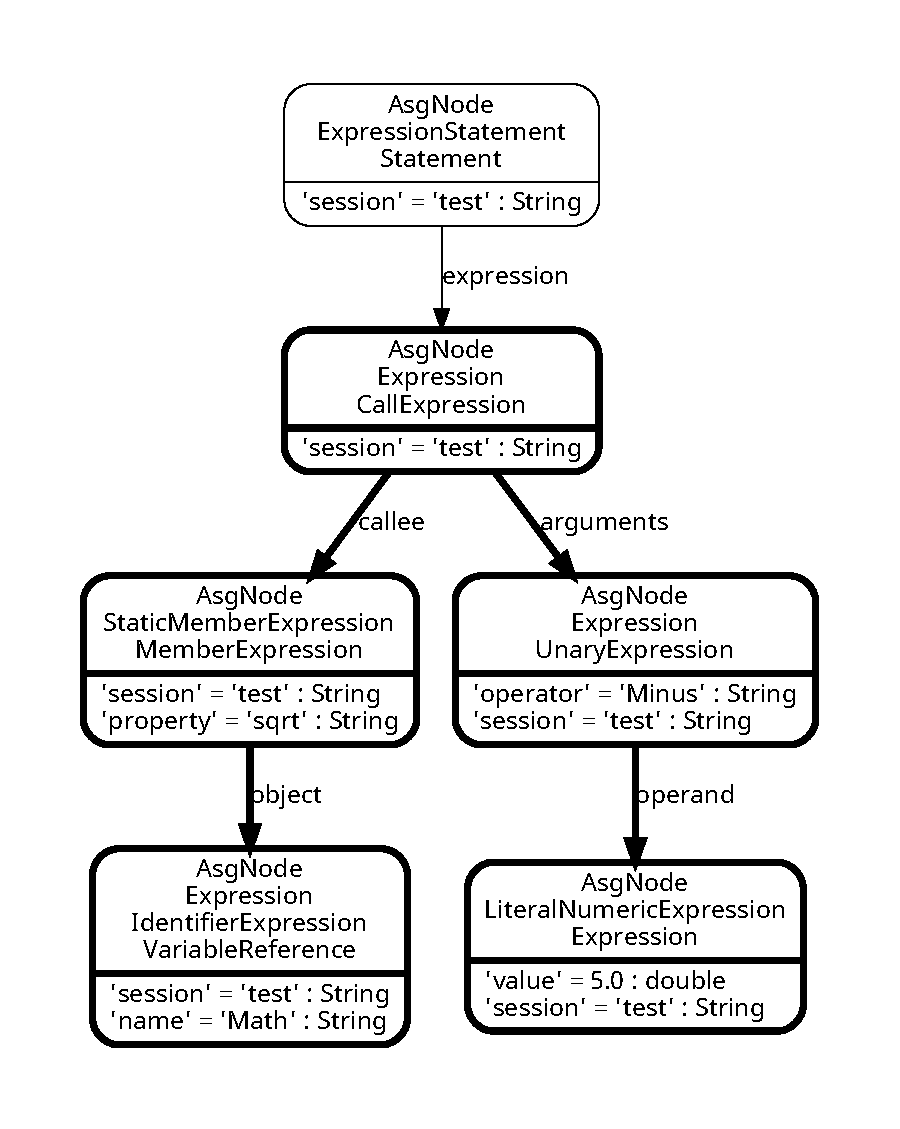
\includegraphics[height=90mm, trim=12mm 12mm 12mm 12mm,clip]{figures/analysis_squareRootArgument.pdf}
	\caption{Matching the \lstinline{squareRootNegativeArgument-literal} analysis pattern}
	\label{fig:analysis-squarerootnegativeargument-simple}
\end{figure}

\Cref{fig:analysis-squarerootnegativeargument-simple} presents a partial ASG demonstrating how a square root called with a negative argument defect is revealed when the argument is a numeric literal. The nodes with thicker outlines are members of the pattern matching expression. The \lstinline{`name'} property of the \lstinline{VariableReference} connected to the \lstinline{StaticMemberExpression} is checked whether it is \lstinline{Math}, the \lstinline{`property'} property of the \lstinline{StaticMemberExpression} is checked whether it is \lstinline{sqrt}, and the \lstinline[keywordstyle={}]{`operator'} property of the \lstinline{UnaryExpression} connected to the \lstinline{LiteralNumericExpression} is checked whether it is \lstinline{Minus}. The source code of the analysis is available in the Appendix.


\section{Complex Analyses with the Qualifier System}

Some defects are more general than to present their patterns in an intact graph directly. Detecting complex errors like these may involve to deduce variable and function return values, and it may require to manipulate the graph to dredge defect patterns for matching. Implementing complex analyses for these defects involved the creation of the Qualifier System, a generic graph constraint propagation strategy for revealing — otherwise generally unmatchable — \emph{transitive} defect patterns. This section details the analyses I implemented for Codemodel-Rifle involving extensive graph manipulations, using the Qualifier System.


\subsection{Transitive Defects}

In this thesis, the term transitive defect is used as follows. A software defect is considered \emph{transitive}, if its effect propagates through multiple variable value assignment and/or function calls. Patterns of transitive defects generally can not be directly matched in the ASG, because the graph pattern of such defects — spanning an indeterminate number of functions or variable assignments — can not be described by one general pattern expression. But, patterns of transitive defects can be deduced in the ASG by following their propagation, and marking the intermediate nodes with constraints.

Demonstratively, the running example presented in \Cref{chapter:background} contains a transitive division by zero defect. In the example's \lstinline{exporter} module, there is a variable given the value zero, then the variable is nested into several levels of variable assignments and function return expressions, finally into the \lstinline{exporter} module's default function export. The exported function will return zero, too. After the example's \lstinline{importer} module imports the default export of \lstinline{exporter}, it divides numeric literal $5$ with the return value of the imported function, practically by zero.

The defect is transitive in the meaning that the zero is not a numeric literal $0$ which could be revealed easily by simple pattern matching. Instead, that zero comes from several levels of nested variable assignments and functions — it \emph{transits} along variable assignments and functions. This transitivity can be deduced by the Qualifier System.

\Cref{fig:transitive-defect-propagation} presents the propagation of the running example's transitive division by zero defect in the \lstinline{exporter} module's partial ASG. The graph node marked with black filling is the exported \lstinline{function b()} (which is the right-hand value of the division in the \lstinline{importer} module). The node with crimson filling is the \lstinline{LiteralNumericExpression}, which finally causes \lstinline{function b()} to return 0. The propagation of the transitive defect starts at the assignment of the literal zero (the crimson node), and ends — at least in the \lstinline{exporter} module — at the exported function (the black node). (Of course, the propagation does not end at module boundaries, since the related modules' ASGs are interconnected. In this case however, the \lstinline{importer} module was omitted from the graph for transparency.)

\begin{sidewaysfigure}[!p]
  \centering
	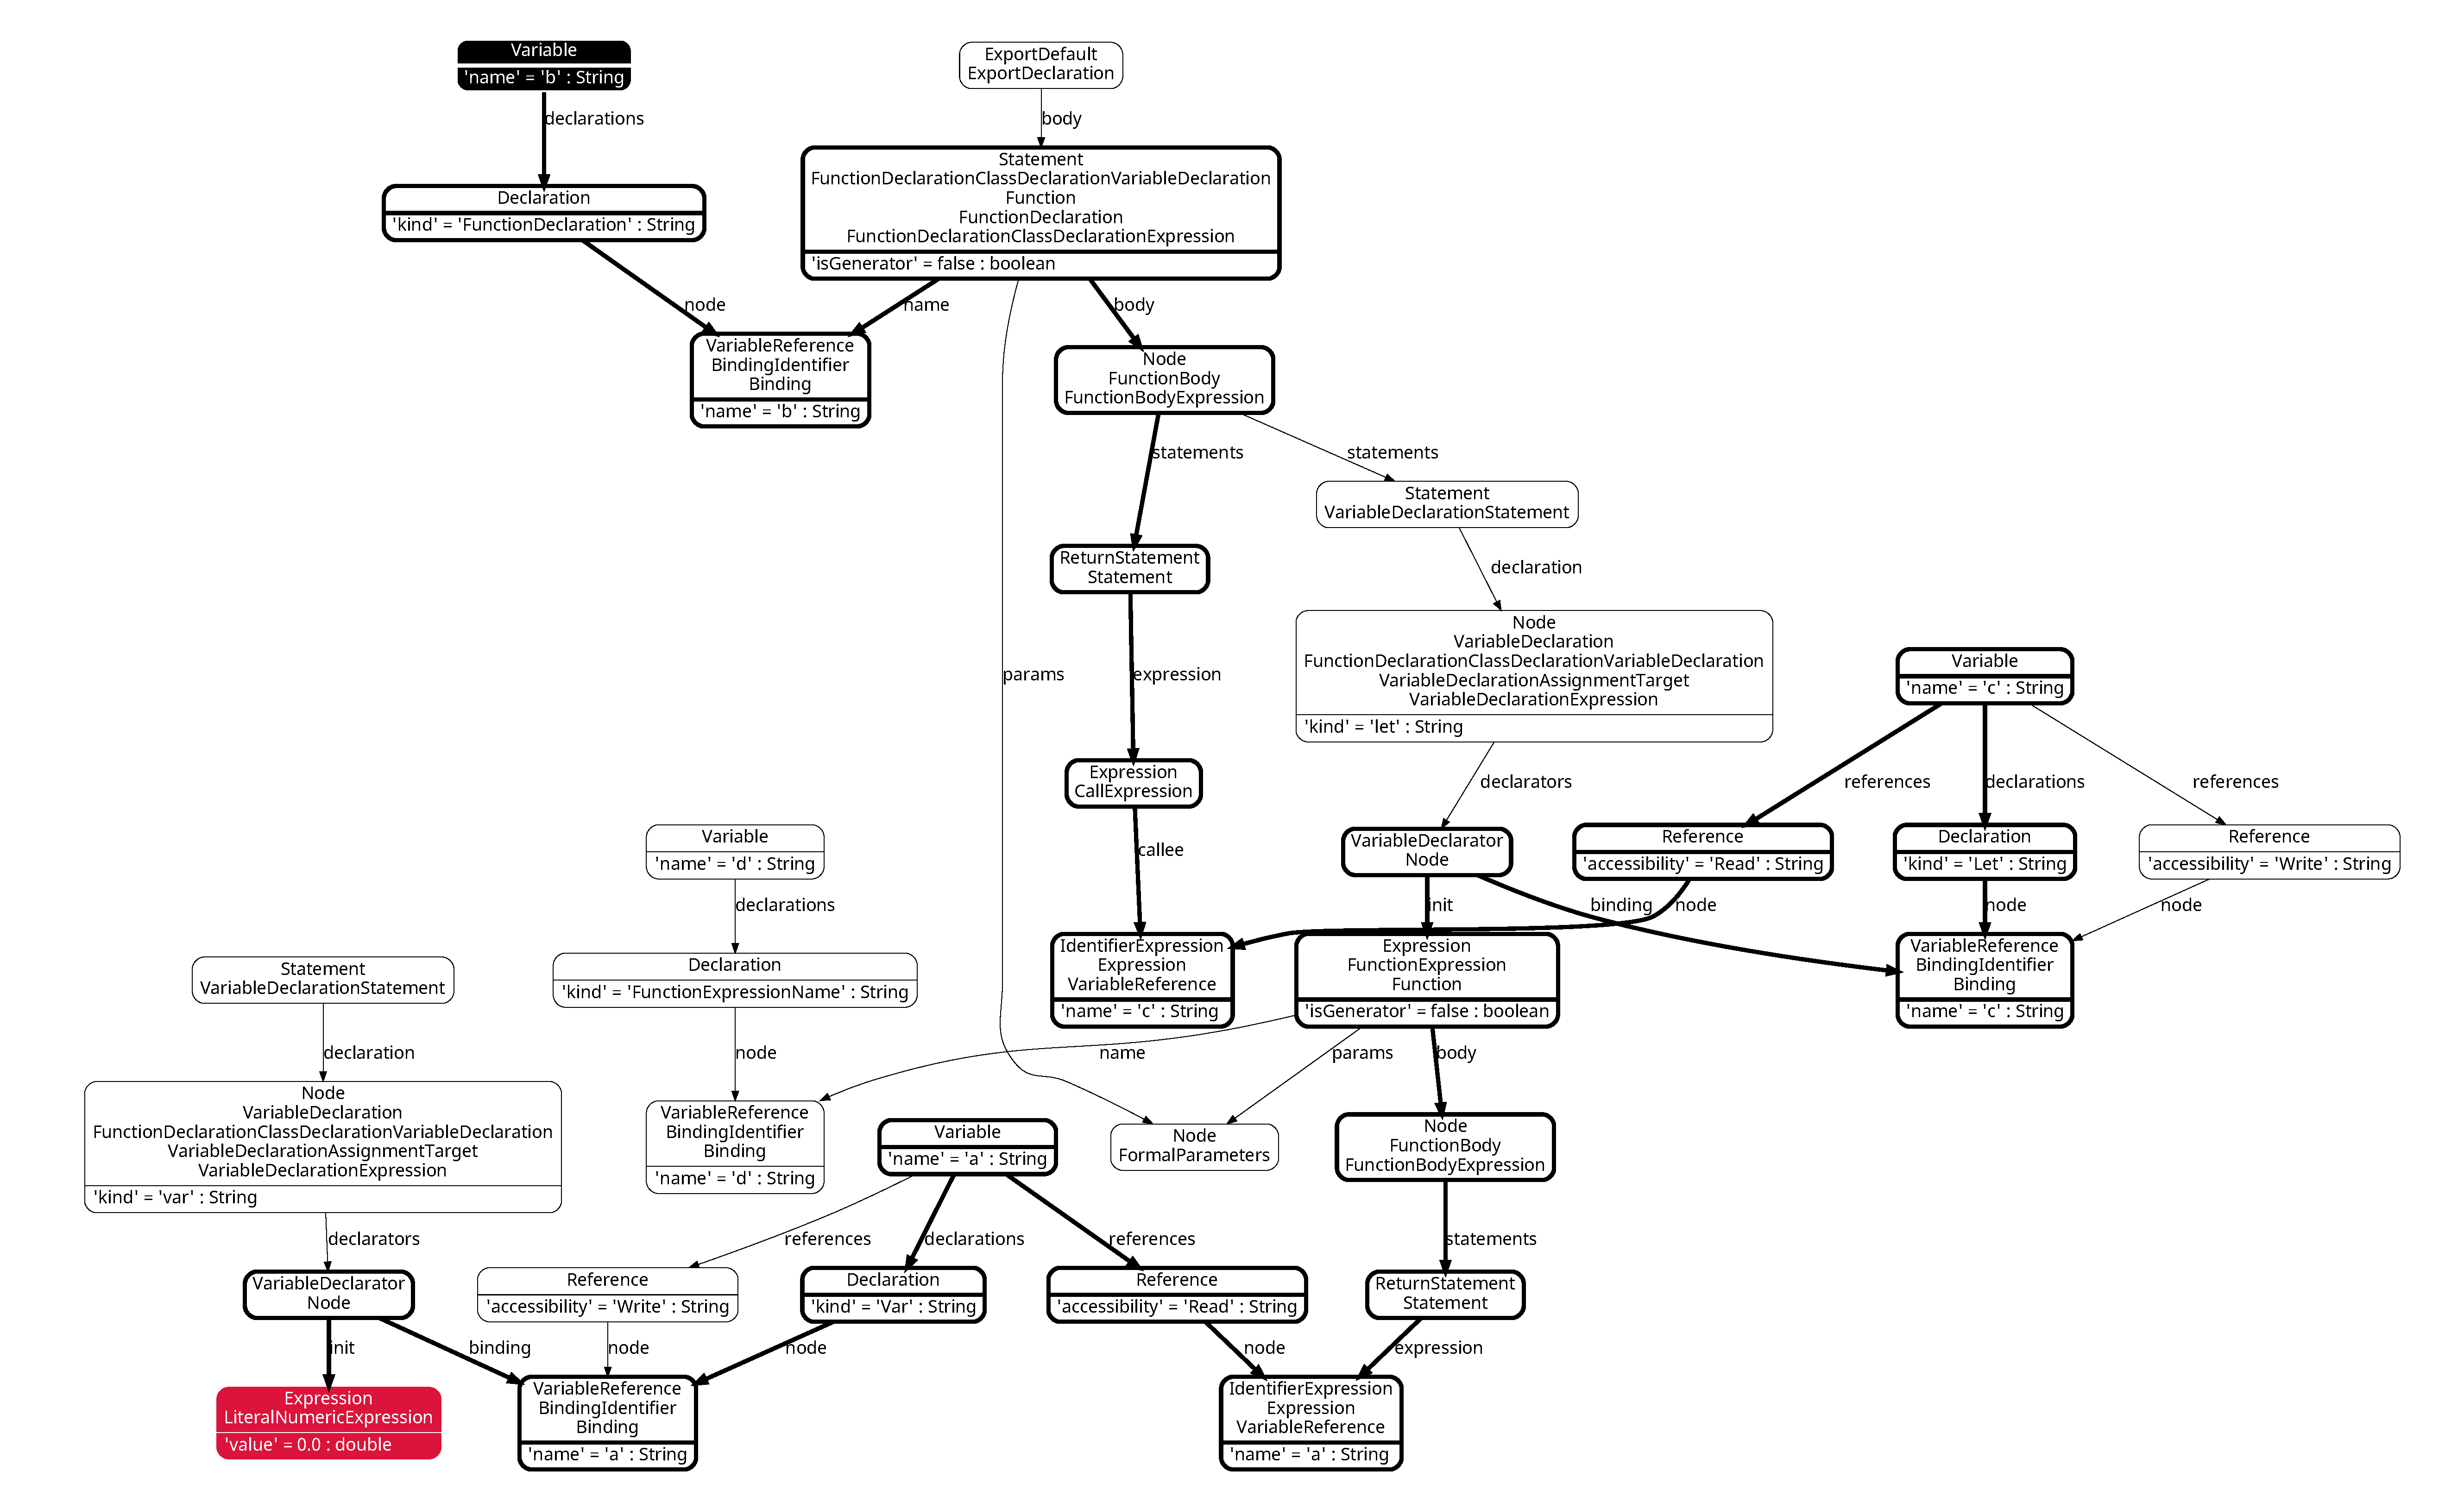
\includegraphics[width=\textwidth, trim=12mm 12mm 12mm 12mm,clip]{figures/transitive-defect-propagation.pdf}
  \caption{The transition path of the running example's division by zero defect}
  \label{fig:transitive-defect-propagation}
\end{sidewaysfigure}


\subsection{Introduction: The Qualifier System}

The Qualifier System is the generalisation of Dániel Stein's Type System~\cite{stein-daniel-msc}. The system assigns well-defined constraints to ASG nodes satisfying certain criteria, then propagates these constraints through the graph by certain rules. These constraints — the \emph{qualifiers} — are \emph{instances} of the Qualifier System: they are represented by graph nodes, connected to a central \lstinline{QualifierSystem} collector node with a \lstinline{:_instance} relationship.

The graph manipulations of the Qualifier System are performed:
\begin{itemize}
\item \textbf{after} the analysed repository is imported/synchronised, the source files' ASGs are constructed, and the related modules' graphs are interconnected to each other,
\item \textbf{before} the defect patterns of the analyses are matched.
\end{itemize}

This allows to first manipulate the graph in several ways by assigning and propagating the qualifiers, and then build pattern matching expressions specifically for the qualifier instances. This way, \emph{transitive} defects — like the running example of \Cref{chapter:background}, where the division by zero is passed along multiple functions and variable assignments — can be detected by deducing the transitions by the qualifiers.

The basic operation of the system is the following. In the enumeration below, the \textbf{phase description} is followed by a concrete demonstrative case based on the running example presented in \Cref{chapter:background}.

\begin{enumerate}
\item \textbf{Initialise the Qualifier System. Create the \lstinline{QualifierSystem} collector node and the qualifier instance nodes.} In the running example, the analysis is based on propagating the \lstinline{EqualsZero} qualifier instance.
\item \textbf{Identify all literals which can be directly marked with a qualifier instance. Connect them to the right qualifier instance with the edge \lstinline{:_qualifier}.} In the running example, it means connecting the \lstinline{LiteralNumericExpression} node of the \lstinline{var a = 0;} variable declaration statement to the \lstinline{EqualsZero} instance.
\item \textbf{Connect adjacent nodes to the same qualifier if they satisfy propagation criteria.} In the running example, it means connecting also the \lstinline{VariableDeclarator} node to the \lstinline{EqualsZero} qualifier instance, because it satisfies the propagation criterion of being connected to a \lstinline{LiteralNumericExpression} by an \lstinline{init} relationship.
\item \textbf{Repeat the previous step until there is no modification in the graph.\footnote{There has to be a stop condition for unintentional infinite loops.}} In the running example — after the propagation finished — the \lstinline{EqualsZero} qualifier will be connected to every entity that is caused to be zero because of the \lstinline{var a = 0;} assignment, including the exported \lstinline{function b()}, and thus the imported \lstinline{defaultName()} function — which is the right-hand side value of the division. Therefore, the transitive division by zero defect can be detected by simply checking whether the right-hand side of the expression has an \lstinline{EqualsZero} qualifier.
\end{enumerate}

If the propagation of the Qualifier System finished, then all transitive defects are \emph{closed} in the meaning that every spread of the defect is marked with a qualifier, so it can be easily detected by a simple pattern matching expression. The following subsections present examples for detecting transitive defects with the Qualifier System.


\subsection{The Running Example's Division By Zero (transitive)}

Detecting a transitive division by zero defect — when the zero expression is not a numeric literal 0, but a variable or a function providing the value zero — requires the right-hand value of the division expression to be deduced. If this value comes from several nested variable assignments and functions, like presented in the running example, the originating value has to be found: a variable assignment with a numeric literal.

Finding a variable assignment, where a numeric literal is the assigned value, can be carried out by simple pattern matching. If this value equals zero, its graph node, the \lstinline{LiteralNumericExpression} is qualified by using an \lstinline{EqualsZero} qualifier instance. After this assignment has been qualified, its adjacent nodes are inspected whether they can be also qualified, according to the propagation rules\footnote{The propagation rules or propagation criteria of Codemodel-Rifle's Qualifier System is implemented as pattern matching queries. Let $N_1$ be qualified by a qualifier instance, and let $N_2$ be an adjacent node of $N_1$ via the relationship $R$. If $R$ is member of the set of qualifier propagator relationships, then $N_2$ gets qualified too.} of the Qualifier System. In the current case, after the \lstinline{LiteralNumericExpression}, its only adjacent ASG node, the \lstinline{VariableDeclaration} gets qualified too by \lstinline{EqualsZero}. This is valid, because the \lstinline{init} edge connecting the two nodes is allowed to propagate an \lstinline{EqualsZero} qualifier instance. After the \lstinline{VariableDeclaration} has been qualified, its adjacent nodes are inspected whether they can be qualified, and the propagation algorithm continues until there are no more paths the qualifier instance could be propagated further on.

In the running example, the propagation of the \lstinline{EqualsZero} qualifier instance stops at the right-hand value of the importer module's division expression. Semantically, the meaning that the right-hand value of the division expression is qualified with an \lstinline{EqualsZero} instance: the division's right-hand side value (the value of the \lstinline{defaultName()} function) has been successfully deduced, and found to be equal to zero.

After the propagation of qualifiers, a simple pattern matching query checks if there are any right-hand values of division expressions qualified by \lstinline{EqualsZero}. If yes, then a division by zero is performed, so it is reported to the developer.

\Cref{fig:divisionbyzero-transitive} presents the propagation of the \lstinline{EqualsZero} qualifier, regarding the running example's transitive division by zero defect. Although the figure is analogous to \Cref{fig:transitive-defect-propagation} by showing the same path, \Cref{fig:transitive-defect-propagation} shows the propagation path of the \emph{defect}, while \Cref{fig:divisionbyzero-transitive} shows the propagation of the \lstinline{EqualsZero} \emph{qualifier}, following the defect.

\begin{sidewaysfigure}[!p]
  \centering
	
\includegraphics[width=\textwidth, trim=12mm 12mm 12mm 12mm,clip]{figures/analysis_divisionByZero_transitive.pdf}
  \caption{The propagation path of the \lstinline{EqualsZero} qualifier instance at analysing the running example}
  \label{fig:divisionbyzero-transitive}
\end{sidewaysfigure}


\subsection{Misuse of Negative Integers as Function Arguments (transitive)}

Detecting the misuse of negative function arguments in trasitive cases — when the argument is not a numeric literal, but a variable, whose value can be anything — needs the same value deduction, as detecting a transitive division by zero defect. The difference is the usage of qualifiers: in this case, a \lstinline{NegativeNumeric} qualifier\footnote{The qualifiers' names can be arbitrary, the semantic design of a qualifier-based analysis requires no predefined naming system. The name of a qualifier instance matters only at implementing the pattern matching algorithms for the analyses: e.g.\ an \lstinline{EqualsZero} qualifier is only an error if it is connected to the right-hand side of a division expression.} is utilised instead of an \lstinline{EqualsZero}.

The \lstinline{NegativeNumeric} qualifier is propagated through the graph along the variable assignments and function return expressions, similarly to the \lstinline{EqualsZero}, with the same stop condition. After the propagation of the qualifier, a simple pattern matching query checks if there are any \lstinline{Math.sqrt()} or \lstinline{Math.log()} function calls with their arguments marked as \lstinline{NegativeNumeric}. If yes, then it is a misuse of negative function argument defect, so it is reported to the developer.


\subsection{Unreachable Code caused by Exception (transitive)}

The exception handling of the \es language has the same semantics as Java. If exceptions thrown with the \lstinline{throw} keyword are surrounded by a \lstinline{try..catch} block context, they get caught, and they can be processed or thrown further.

\begin{figure}[!htb]
	\centering
	\begin{lstlisting}[language=JavaScript]
						function throwsException() {
						    return function () {
						        throw new SQLException;
						    };
						}
						let a = throwsException;
						let b = function () {
						    return function () {
						        let c = throwsException();
						        return 42;
						    }
						};
						console.log(b());
						console.log(42);
	\end{lstlisting}
  \caption{Deeply nested exception in \es}
  \label{fig:deeply-nested-exception}
\end{figure}

An exception halts the execution of the program, and yields it to the exception handler — the catch block —, at least if there are handlers implemented by the developer. Source code following an exception throwing statement is not executed, therefore it is unreachable code. Most static analysis tools detect dead code caused by exceptions, but only very shallowly.

\Cref{fig:deeply-nested-exception} presents a program with an exception nested into several levels of functions. The program — instead of logging 42 to the console — will halt, since calling \lstinline{function b()} will eventually cause an \lstinline{SQLException} to be thrown.

By introducing the \lstinline{ExceptionThrown} qualifier instance into the Qualifier System, the propagation path of an exception can be tracked. At analysing the code of \Cref{fig:deeply-nested-exception}, first the \lstinline{throw new SQLException} statement gets marked by the \lstinline{ExceptionThrown} qualifier. Then after several steps of propagation, \lstinline{function b()} also gets marked, therefore it can be easily found by pattern matching. My analysis reports that:

\begin{itemize}
\item an exception is thrown at the execution of the statement \lstinline{console.log(b())}, and
\item because of the exception, the statement \lstinline{console.log(42)} will never be executed.
\end{itemize}


\section{Limitations of the Analyses}

Though the graph-based static analysis approach is a promising novelty from several aspects, my analyses presented in this thesis are very limited in many ways. Implementing \es module interconnections and introducing the Qualifier System were both relevant acts, but they are only supporting elements of the analyses themselves.

Codemodel-Rifle's variable and function value deductions are primitive: no arithmetic operations are supported, the framework tracks only raw, unmodified values. Conditional cases are not covered either: an exception gets detected only if it is unconditionally thrown.

Implementing sound and complete analyses with the Codemodel-Rifle framework is not a subject of this thesis. But — building upon the work of Dániel Stein — the first steps have been made to create a versatile graph-based static analysis tool capable of inspecting enterprise-grade source code repositories coherently.
\chapter{Evaluation of Performance}
\label{chapter:evaluation}

In this chapter, I evaluate the framework's performance by measuring the duration of analysing several source code repositories.


\section{Evaluation Environment}

\subsection{Computer Configuration}

The measurements were performed on my computer for the sake of simplicity. During a measurement session, my computer was plugged in, it was configured to utilise its full performance, and only those software were running, which were explicitly necessary for the measurements. Each measurement session was preceded by a full system restart.

The major points of the my computer's configuration are the following:

\begin{itemize}
\item \textbf{Brand and model:} Apple MacBook Pro, Mid-2014, 13 inches;
\item \textbf{CPU:} Intel Core i5 (4278U), 2.6 GHz;
\item \textbf{Memory:} 8 GB 1600 MHz DDR3 RAM;
\item \textbf{Storage:} 250 GB SSD.
\end{itemize}


\subsection{Software Configuration}

As currently the Codemodel-Rifle framework does not have any interface to interact with, the measurements were performed as per-repository unit tests with logging test results onto the console.

\begin{itemize}
\item \textbf{Runtime:} JetBrains IntelliJ IDEA Ultimate 2016.3.4
\item \textbf{Java Runtime Environment:} 1.8.0\_112-release-408-b6 x86\_64
\item \textbf{Java Virtual Machine:} OpenJDK 64-Bit Server VM by JetBrains s.r.o (initial memory allocation pool: 4 GB, maximum memory allocation pool: 8 GB)
\item \textbf{Database:} Neo4j Community Edition 3.1.3 Server (initial heap size: 4 GB, maximum heap size: 8 GB, page cache size: 8 GB, transaction log retention policy: 1 day)
\item \textbf{Database driver:} Neo4j Bolt driver for Java 1.1.1
\end{itemize}

For better performance, a database index was defined in Neo4j for the \lstinline{`id'} property of all nodes labeled with \lstinline{'AsgNode'} (practically all nodes created by Codemodel-Rifle).


\section{Measurement Goals and Methods}

\subsection{Selection Criteria of the Analysed Source Code Repositories}

The evaluation was performed on popular open-source JavaScript code repositories randomly chosen and downloaded from GitHub, and on a closed-source, security-oriented industrial project from Tresorit, called \lstinline{webclient}. The altogether 40 repositories differ in size, in the number of lines of code, and in the number of distinct source files.


\subsection{Key Performance Indices}

The goal of the performance evaluation was to determine the time characteristics of the extended Codemodel-Rifle framework, especially the implemented analyses. Based on the production operation of the framework detailed in the introduction of \Cref{chapter:elaboration}, the following Key Performance Indices have been determined to be measured.

\begin{itemize}
\item \textbf{The duration of synchronisation:} the time period between starting the importing process of a code repository (excl. finding all \lstinline{.js} files, and reading the contents of the source files) and saving the last module's last \lstinline{AsgNode} into the database.
\item \textbf{The duration of interconnection:} this time period encompasses searching for semantically valid interconnections amongst related modules' property graphs, and actually performing the interconnections.
\item \textbf{The duration of running the Qualifier System:} this time period encompasses initialising the Qualifier System, and propagating the qualifiers.
\item \textbf{The duration of performing the analyses:} this time period encompasses trying to match all predefined analysis patterns.
\item \textbf{The total duration of the analysis process:} the calculated sum of the above four.
\end{itemize}

Besides the Key Performance Indices, the number of graph nodes and relationships created during the synchronisation of a repository is also recorded.


\subsection{Process of Measurement}

All analysed code repositories were measured four times in a session in order to avoid biases caused by the environment. Each session was preceded by a full system restart. The final measurement results of a repository are averaged from the four different values.


\section{Measurement Results}

In this section, I present and evaluate the measurement results of the aforementioned Key Performance Indices.


\subsection{Synchronisation}

At first, a repository needs to be synchronised into Codemodel-Rifle. In this phase, the source code files of the repository get translated to distinct, per-module property graphs.

\begin{figure}[!htb]
	\centerfloat
	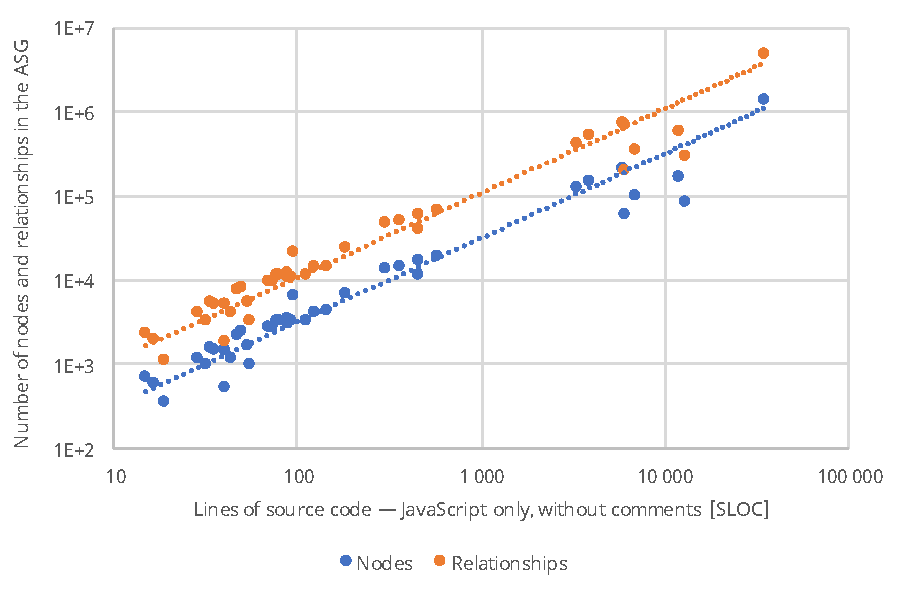
\includegraphics[width=\textwidth,clip]{figures/measurement-nodes-relationships-sloc.pdf}
	\caption{The characteristics of synchronising repositories into Codemodel-Rifle}
	\label{fig:measurement-nodes-relationships-sloc}
\end{figure}

There are many coding styles and conventions, and the contents of the source files can vary from per-line exported configuration constants to program codes without physical line breaks. Nevertheless, there is a linear relationship between the number of code lines and the number of created ASG nodes and relationships in the analysed repositories.

\Cref{fig:measurement-nodes-relationships-sloc} presents the correlation of the source lines of code (SLOC) and the number of ASG nodes and relationships created during synchronising the code bases into Codemodel-Rifle. In terms of SLOC, the smallest repository imported was \lstinline{initialstate/silent-doorbell} with 15 lines of code (686 nodes and 2,306 relationships), while the largest was \lstinline{tresorit/webclient} with 34,546 lines of code (1,346,776 nodes and 4,576,319 relationships).


\begin{figure}[!htb]
	\centerfloat
	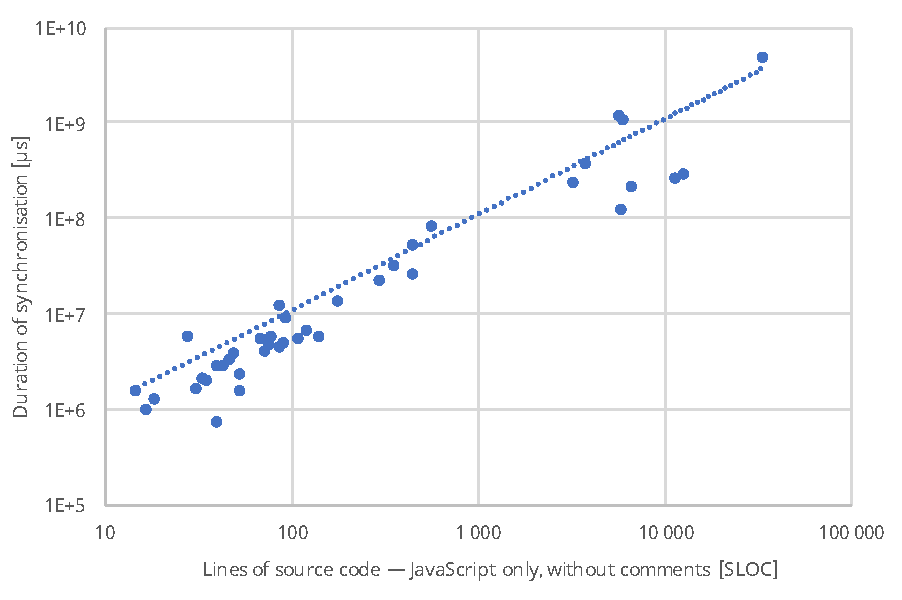
\includegraphics[width=\textwidth,clip]{figures/measurement-synctime-sloc.pdf}
	\caption{The characteristics of synchronising repositories into Codemodel-Rifle}
	\label{fig:measurement-synctime-sloc}
\end{figure}

\begin{figure}[!htb]
	\centerfloat
	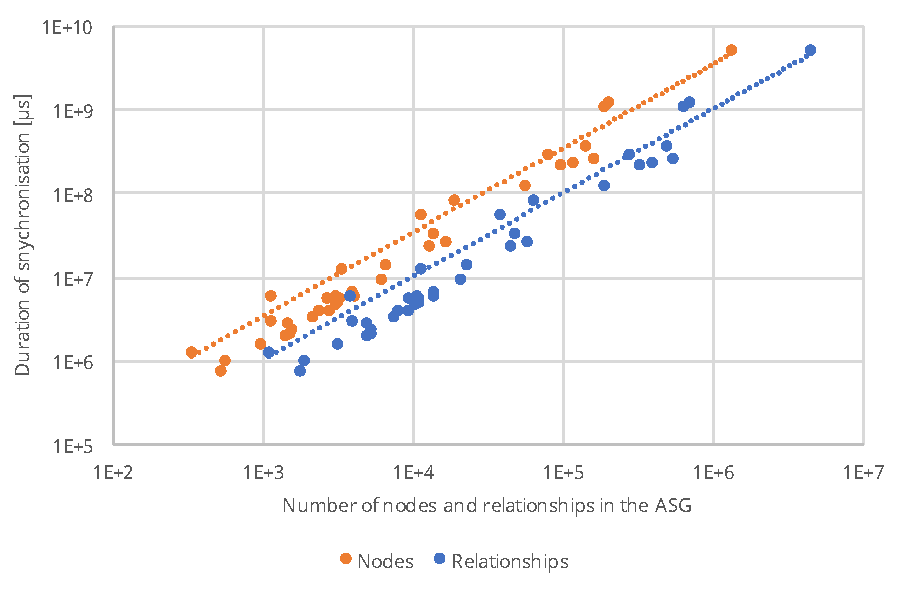
\includegraphics[width=\textwidth,clip]{figures/measurement-synctime-nodes-relationships.pdf}
	\caption{Synchronising repositories into Codemodel-Rifle}
	\label{fig:measurement-synctime-nodes-relationships}
\end{figure}

As for the duration of the synchronisation phase, the tendency is linear in this case too. The bigger the repository is, the more time it consumes to synchronise the code base into Codemodel-Rifle (as more graph nodes and relationships need to be created). \Cref{fig:measurement-synctime-sloc} shows the correlation between the duration of synchronisation and the repository size. The shortest synchronisation duration belongs to the \lstinline{facundoolano/promise-log} repository with altogether 41 SLOC in 1 module, it was imported into the framework in around 7 milliseconds. The import of the largest repository, \lstinline{tresorit/webclient} with 34,546 SLOC in 609 modules, took about 78 minutes.

A more evident approach is to inspect the relationship between the duration of synchronisation and the repository size, but now the latter in terms of the number of created graph nodes and relationships. As \Cref{fig:measurement-synctime-nodes-relationships} shows, the relationship between these two measurement values is also linear. Practically, this means the underlying graph database, Neo4j is able to handle node and relationship creations at very large volumes — even at the magnitude of several millions of graph nodes — linearly. With the effect of the database index on the \lstinline{`id'} attribute, the nodes are retrieved faster at creating the relationships.

An important thing to consider regarding Neo4j is transaction granularity. According to my experience with the production server run on my laptop with the configuration mentioned earlier, the graph database tends to freeze if a very large amount of queries are committed within one transaction. In the framework's current implementation, it is not possible to configure the maximum number of queries committed in one turn. It is hard-coded into the framework to handle each file in a separate transaction as a whole, to preserve at least file-level consistency. The transactions of synchronising larger files (several hundred kilobytes, several thousand SLOC) should be configurably split into multiple smaller ones in the future, in order to ensure solid operation.


\subsection{Interconnection}

In theory, interconnecting \es modules is a very slow operation. The 13 implemented interconnection algorithms are run one by one, each matching two complex graph patterns for finding the compatible export and import cases.

In practice, however, the interconnection phase was the fastest of all. Even at the largest analysed repository, \lstinline{tresorit/webclient}, having 609 distinct \es modules, 1,346,776 graph nodes and 4,576,319 graph relationships, the interconnection phase took less than 30 seconds. At smaller repositories, or at repositories having only one module, the duration the interconnection phase was a small, sub-second value.

Regarding the characteristics of the export-import interconnections, no explicit relationship can be determined between the repository size or the number of modules and the duration of the interconnection phase. This is understandable: altering the number of distinct modules in an \es project does not necessarily cause the number of \emph{related} modules to change.

\begin{figure}[!htb]
	\centerfloat
	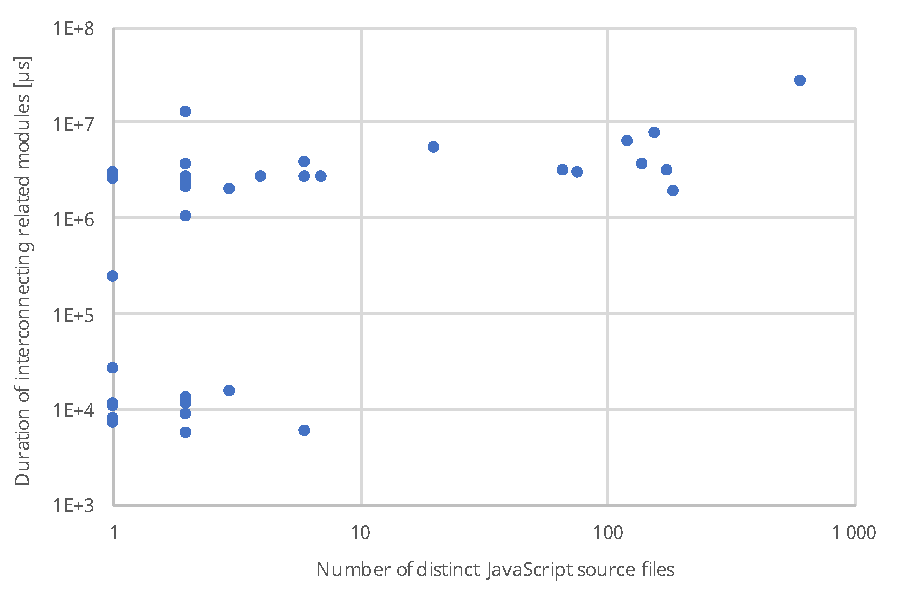
\includegraphics[width=\textwidth,clip]{figures/measurement-interconnecttime-modules.pdf}
	\caption{The characteristics of interconnecting related modules}
	\label{fig:measurement-interconnecttime-modules}
\end{figure}

\Cref{fig:measurement-interconnecttime-modules} shows the duration of interconnecting related modules in the light of the number of distinct modules in the repository. The figure shows that no relationship can be determined between the two values. Since the design of modularisation varies for every project, simply the number of distinct modules does not indicate how many of those modules are related to each other.


\subsection{The Qualifier System}

Spreading qualifiers along possible propagation paths in the Abstract Semantic Graph is a long process. In each propagation step, a particular qualifier can traverse only one relationship at a time — similarly to solving data-flow equations locally, based on the solution of the preceding equation. In larger graphs containing long transitive paths, producing a full transitive closure can involve many steps.

The more \textquote{entry points} has a particular software for the Qualifier System (e.g.\ literals and \lstinline{throw} statements can be entry points: they are the first to be marked with a qualifier at the initialisation of the Qualifier System), the more propagation paths need to be closed up. The bigger the repository is, the more likely it is to contain such entry points.

\begin{figure}[!htb]
	\centerfloat
	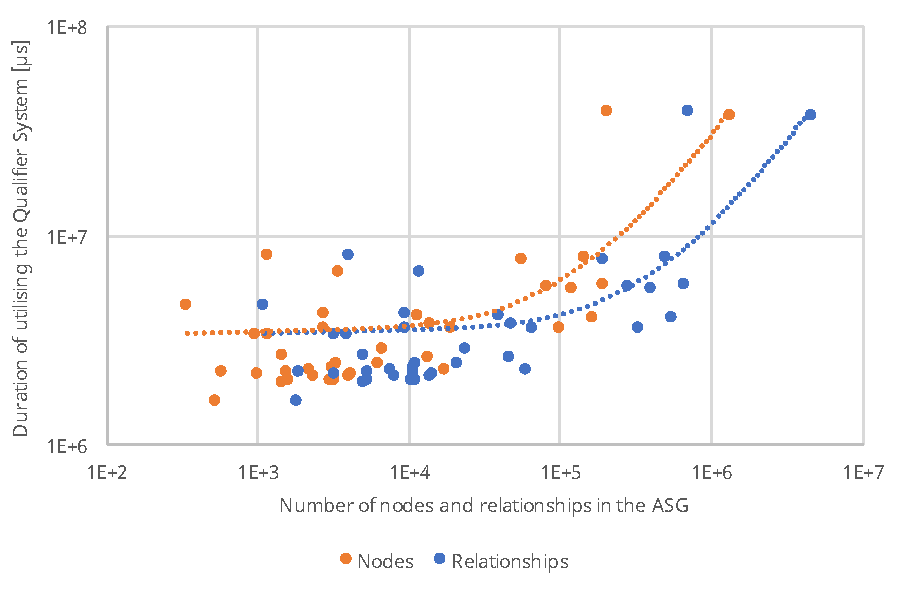
\includegraphics[width=\textwidth,clip]{figures/measurement-qualifiersystem-nodes-relationships.pdf}
	\caption{The characteristics of running the Qualifier System}
	\label{fig:measurement-qualifiersystem-nodes-relationships}
\end{figure}

\Cref{fig:measurement-qualifiersystem-nodes-relationships} presents the characteristics of the Qualifier System. The relationship between the duration of running the Qualifier System and the number of nodes and relationships in the ASG is not unequivocal, but an exponential trendline fits the dataset well. The Qualifier System's longest run took 38 seconds, at analysing the \lstinline{alvin198761/web-os} repository. For the \lstinline{tresorit/webclient}, the Qualifier System ran for 36 seconds. It is worth to mention here, that while the \lstinline{web-os} contains only 5,922 SLOC, the \lstinline{webclient} has 34,546. The similar duration of running the Qualifier System with this difference could imply that the \lstinline{web-os} contains much more transitive defect paths to propagate qualifiers on.


\subsection{Analysis}

Importing, interconnecting, and applying the Qualifier System are only preparatory steps for running the actual analyses. All analyses involve matching complex patterns, even the ones using the results of the Qualifier System: besides qualifiers, several other attributes need to be queried for returning a complete set of analysis results, like code location information, and the containing module's file path.

\Cref{fig:measurement-analysis-nodes-relationships} presents the characteristics of the analyses. The duration of the analysis phase seemingly does not have any relationship with the number of graph nodes and relationships of a code repository. This is plausible, since the number of defects in a repository does not necessarily depend on the code base's size.

\vspace*{-2mm}
\begin{figure}[!htb]
	\centerfloat
	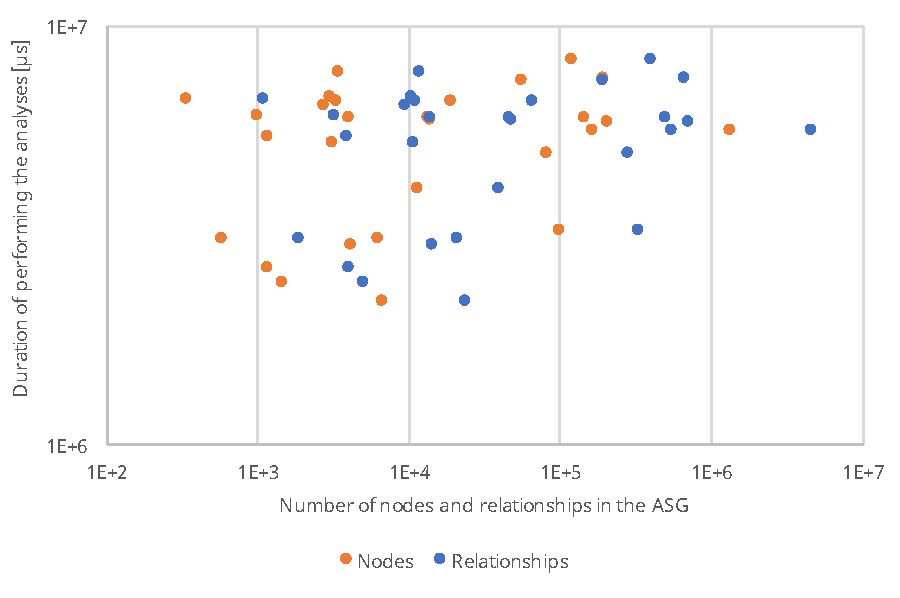
\includegraphics[width=\textwidth,clip]{figures/measurement-analysis-nodes-relationships.pdf}
	\caption{The characteristics of performing the analyses}
	\label{fig:measurement-analysis-nodes-relationships}
\end{figure}
\vspace*{-2mm}

\subsection{Total Duration of the Analysis Process}

The total duration of analysing a repository seems to be in linear relationship with the repository's size. \Cref{fig:measurement-totaltime-sloc} and \Cref{fig:measurement-totaltime-nodes-relationships} present that both measured in SLOC and in the number of graph nodes and relationships, there is a linear tendency: the bigger the source code repository is, the more time it takes perform a complete analysis process on it.

It is interesting to notice by the detailed measurement data in the Appendix, how the proportion of the synchronisation phase's duration within the duration of the full analysis process increases with the size of the repository. While for the smaller repositories, the import makes up only 30–40\% of the total duration, for the larger repositories, it increases to 80–90\%. For the \lstinline{tresorit/webclient} repository, the synchronisation phase alone makes up 98\% of the duration of the total analysis process.

\begin{figure}[!p]
	\centerfloat
	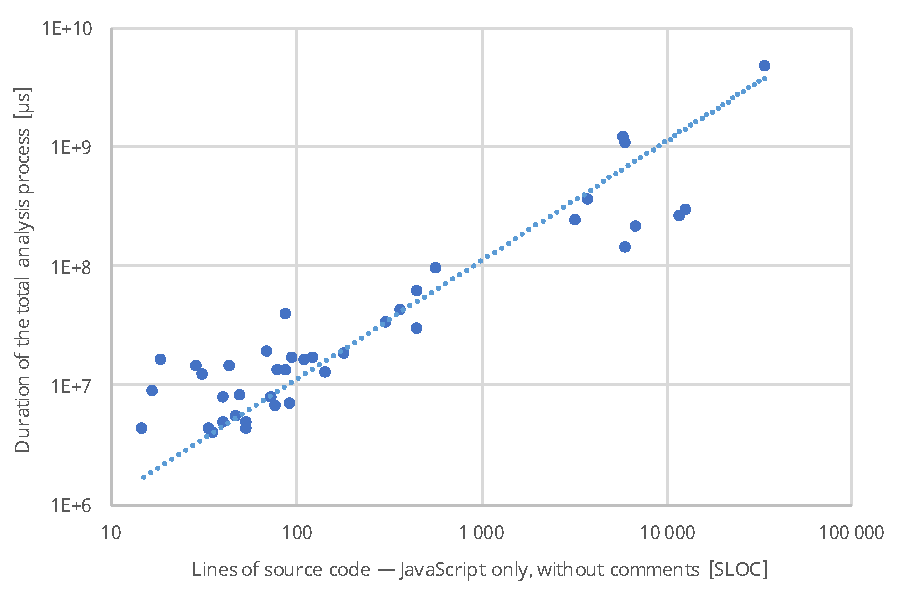
\includegraphics[width=\textwidth-1cm,clip]{figures/measurement-totaltime-sloc.pdf}
	\caption{The characteristics of the full analysis process}
	\label{fig:measurement-totaltime-sloc}
\end{figure}

\begin{figure}[!p]
	\centerfloat
	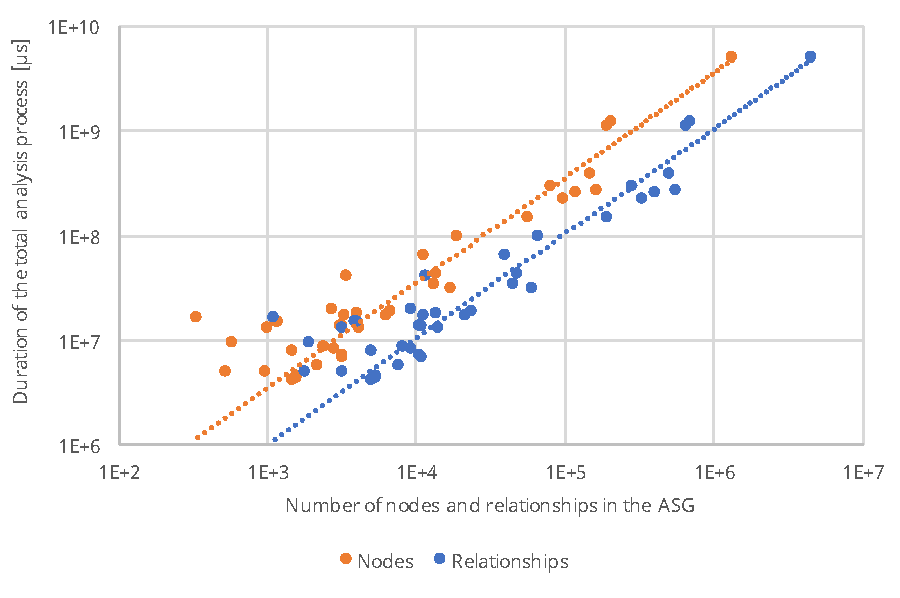
\includegraphics[width=\textwidth-1cm,clip]{figures/measurement-totaltime-nodes-relationships.pdf}
	\caption{The characteristics of the full analysis process}
	\label{fig:measurement-totaltime-nodes-relationships}
\end{figure}


\section{Defects Found by the Framework}

The framework detected only two types of defects in the 40 analysed repositories: 897 cases of uninitialised variables, and 134 cases of globally unused exports were found. As the analysis is neither sound, nor complete, these numbers can be inaccurate. However, I inspected a randomly chosen subset of the found defects manually, and — according to my experience — the defects were indeed present in all cases.


\section{Threats to Validity}

I designed the measurements to be as accurate and complete as possible. Nevertheless, there are factors which I could not fully control, and these may have influenced the results. In this section, I summarise the factors which could bias the measurements.


\paragraph{Measurements on a Consumer Laptop}
Since my computer runs an operating system targeted for consumer usage, it may contain software running in the background, which influence measurement factors like processor or memory usage. I tried to mitigate this by configuring the computer to utilise all resources for the measurement procedure, by running the measurements multiple times, and by analysing a larger number of code repositories independently.


\paragraph{Graph Query Optimisations}
I tried to optimise the graph queries of the interconnections and the analyses as much as I could. However, since I am not an expert in the internals of Cypher queries, it is possible that some queries can be optimised further. Therefore, the characteristics of the interconnections or the analyses may not be fully correct.


\paragraph{Methological Mistakes}
It is possible that I made other methodological mistakes at implementing the analyses or the measurements. Using a fluid, internal semantics for the interconnection of modules incorrectly can be an example of a such mistake.
\chapter{Conclusion and Future Work}
\label{chapter:conclusion}

My primary object was to extend the Codemodel-Rifle framework with analysis algorithms. To make the framework practically usable, this involved several other supporting features to be planned and implemented.

Codemodel-Rifle was rearchitectured to become modular. Therefore, by changing components if necessary, the framework can adapt to various requirements and use-cases. The software was also revised semantically, by elaborating the capability of performing analyses on multiple modules coherently, the Qualifier System, and the analyses themselves.

Once the framework contains enough analyses, it can be a practical tool for helping developers in finding defects. By this time, utilising module interconnections and the Qualifier System, it is expressive enough to cover a large set of statically analysable use-cases.


\section{Summary of Contributions}

I contributed to the development of the framework in two ways. Scientific (or semantic) contributions encompass the performances regarding the analysis of \es, and the language itself. Engineering contributions cover designing the architecture of a large-scale, modular code analysis software, and implementing a proof-of-concept prototype.


\subsection{Scientific Contributions}

I have achieved the following scientific contributions:

\begin{itemize}
\item Defined the semantics of interconnecting multiple Abstract Semantic Graphs along the export-import statements of the \es language.
\item Proposed an approach to evaluate graph-based static analyses over multiple \es modules coherently.
\item Provided an extensible data model and an algorithm for analysing the data flow of \es software.
\end{itemize}


\subsection{Engineering Contributions}

I have also achieved the following engineering contributions:

\begin{itemize}
\item Designed a modular architecture for an analysis framework to be capable to scale and adapt to various requirements.
\item Created a specialised Object-Graph Mapping layer for optimising the transformation of Abstract Syntax Trees into Abstract Semantic Graphs.
\item Implemented a specialised Query Builder for the Cypher language.
\item Elaborated several graph-based analyses for the \es language.
\end{itemize}


\section{Future Work}

The goal of the work described in this thesis was to extend the Codemodel-Rifle framework with analysis algorithms. By implementing several other supporting features, the scope broadened: it is now possible to analyse multiple modules coherently, and to inspect the data flow of \es software. Implementing more — and more precise — analyses, which utilise these new capabilities is a task for the future.

Further optimisations can be done at various points of the architecture. By collaborating with version-control systems like Git for file-level incremental processing, the speed of the analyses could be increased significantly.

To include Codemodel-Rifle into various software development methods, the framework should be able to communicate with other software. Thus the capability of producing machine-readable output is to be implemented. Also, creating plugins for continuous integration infrastructures would make possible to embed the framework into well-known software production architectures.
\chapter*{Acknowledgements}
\phantomsection
\addcontentsline{toc}{chapter}{Acknowledgements}
\thispagestyle{plain}

%%% Local Variables:
%%% mode: latex
%%% TeX-master: "main"
%%% End:

\printbibliography

\appendix
\chapter*{Appendix}
\phantomsection
\addcontentsline{toc}{chapter}{Appendix}
\renewcommand{\thesection}{\Alph{section}}

\section{Cypher Queries for Interconnecting the ASGs of Related Modules}

\subsection{exportAlias–importAlias}
\begin{lstlisting}[language=Cypher]
MATCH
// exporter.js: export { name1 as exportedName1 };
    (exporter:CompilationUnit)-[:contains]->(:ExportLocals)
        -[:namedExports]->(exportLocalSpecifier:ExportLocalSpecifier)
        -[:name]->(:IdentifierExpression)
        <-[:node]-(:Reference)
        <-[:references]-(:Variable)
        -[:declarations]->(declarationToMerge:Declaration)
        -[:node]->(:BindingIdentifier),

// importer.js: import { exportedName1 as importedName1 } from "exporter";
    (importer:CompilationUnit)-[:contains]->(import:Import)
        -[:namedImports]->(importSpecifier:ImportSpecifier)
        -[:binding]->(importBindingIdentifierToMerge:BindingIdentifier)
        <-[:node]-(declarationToDelete:Declaration)
        <-[:declarations]-(importedVariable:Variable)

    WHERE
    exporter.parsedFilePath CONTAINS import.moduleSpecifier
    AND exportLocalSpecifier.exportedName = importSpecifier.name

MERGE
    (importedVariable)-[:declarations]->(declarationToMerge)
        -[:node]->(importBindingIdentifierToMerge)

DETACH DELETE
    declarationToDelete
\end{lstlisting}


\newpage
\subsection{exportAlias–importDefault}
\begin{lstlisting}[language=Cypher]
MATCH
// exporter.js: export { name1 as default };
    (exporter:CompilationUnit)-[:contains]->(:ExportLocals)
        -[:namedExports]->(exportLocalSpecifier:ExportLocalSpecifier)
        -[:name]->(:IdentifierExpression)
        <-[:node]-(:Reference)
        <-[:references]-(:Variable)
        -[:declarations]->(declarationToMerge:Declaration)
        -[:node]->(:BindingIdentifier),

// importer.js: import defaultName from "exporter";
    (importer:CompilationUnit)-[:contains]->(import:Import)
        -[:defaultBinding]->(importBindingIdentifierToMerge:BindingIdentifier)
        <-[:node]-(declarationToDelete:Declaration)
        <-[:declarations]-(importedVariable:Variable)

    WHERE
    exporter.parsedFilePath CONTAINS import.moduleSpecifier
    AND exportLocalSpecifier.exportedName = 'default'

MERGE
    (importedVariable)-[:declarations]->(declarationToMerge)
        -[:node]->(importBindingIdentifierToMerge)

DETACH DELETE
    declarationToDelete
\end{lstlisting}


\newpage
\subsection{exportAlias–importName}
\begin{lstlisting}[language=Cypher]
MATCH
// exporter.js: export { name1 as exportedName1 };
    (exporter:CompilationUnit)-[:contains]->(:ExportLocals)
        -[:namedExports]->(exportLocalSpecifier:ExportLocalSpecifier)
        -[:name]->(:IdentifierExpression)
        <-[:node]-(:Reference)
        <-[:references]-(:Variable)
        -[:declarations]->(declarationToMerge:Declaration)
        -[:node]->(:BindingIdentifier),

// importer.js: import { exportedName1 } from "exporter";
    (importer:CompilationUnit)-[:contains]->(import:Import)
        -[:namedImports]->(:ImportSpecifier)
        -[:binding]->(importBindingIdentifierToMerge:BindingIdentifier)
        <-[:node]-(declarationToDelete:Declaration)
        <-[:declarations]-(importedVariable:Variable)

    WHERE
    exporter.parsedFilePath CONTAINS import.moduleSpecifier
    AND exportLocalSpecifier.exportedName = importBindingIdentifierToMerge.name

MERGE
    (importedVariable)-[:declarations]->(declarationToMerge)
        -[:node]->(importBindingIdentifierToMerge)

DETACH DELETE
    declarationToDelete
\end{lstlisting}


\newpage
\subsection{exportDeclaration–importAlias}
\begin{lstlisting}[language=Cypher]
MATCH
// exporter.js: export var name1;
    (exporter:CompilationUnit)-[:contains]->(:ExportDeclaration)
        -[:declaration]->
        (:FunctionDeclarationClassDeclarationVariableDeclaration)
        -[:declarators]->(:VariableDeclarator)
        -[:binding]->(exportBindingIdentifier:BindingIdentifier)
        <-[:node]-(declarationToMerge:Declaration)
        <-[:declarations]-(:Variable),

// importer.js: import { name1 as importedName1 } from "exporter";
    (importer:CompilationUnit)-[:contains]->(import:Import)
        -[:namedImports]->(importSpecifier:ImportSpecifier)
        -[:binding]->(importBindingIdentifierToMerge:BindingIdentifier)
        <-[:node]-(declarationToDelete:Declaration)
        <-[:declarations]-(importedVariable:Variable)

    WHERE
    exporter.parsedFilePath CONTAINS import.moduleSpecifier
    AND exportBindingIdentifier.name = importSpecifier.name

MERGE
    (importedVariable)-[:declarations]->(declarationToMerge)
        -[:node]->(importBindingIdentifierToMerge)

DETACH DELETE
    declarationToDelete
\end{lstlisting}


\newpage
\subsection{exportDeclaration–importName}
\begin{lstlisting}[language=Cypher]
MATCH
// exporter.js: export var name1;
    (exporter:CompilationUnit)-[:contains]->(:ExportDeclaration)
        -[:declaration]->
        (:FunctionDeclarationClassDeclarationVariableDeclaration)
        -[:declarators]->(:VariableDeclarator)
        -[:binding]->(exportBindingIdentifier:BindingIdentifier)
        <-[:node]-(declarationToMerge:Declaration)
        <-[:declarations]-(:Variable),

// importer.js: import { name1 } from "exporter";
    (importer:CompilationUnit)-[:contains]->(import:Import)
        -[:namedImports]->(importSpecifier:ImportSpecifier)
        -[:binding]->(importBindingIdentifierToMerge:BindingIdentifier)
        <-[:node]-(declarationToDelete:Declaration)
        <-[:declarations]-(importedVariable:Variable)

    WHERE
    exporter.parsedFilePath CONTAINS import.moduleSpecifier
    AND exportBindingIdentifier.name = importBindingIdentifierToMerge.name

MERGE
    (importedVariable)-[:declarations]->(declarationToMerge)
        -[:node]->(importBindingIdentifierToMerge)

DETACH DELETE
    declarationToDelete
\end{lstlisting}


\newpage
\subsection{exportDefaultDeclaration–importAlias}
\begin{lstlisting}[language=Cypher]
MATCH
// exporter.js: export default name1;
    (exporter:CompilationUnit)-[:contains]->(:ExportDefault)
        -[:body]->(:FunctionDeclarationClassDeclarationVariableDeclaration)
        -[:name]->(exportBindingIdentifier:BindingIdentifier)
        <-[:node]-(declarationToMerge:Declaration)
        <-[:declarations]-(exportedVariable:Variable),

// importer.js: import { name1 as importedName1 } from "exporter";
    (importer:CompilationUnit)-[:contains]->(import:Import)
        -[:namedImports]->(importSpecifier:ImportSpecifier)
        -[:binding]->(importBindingIdentifierToMerge:BindingIdentifier)
        <-[:node]-(declarationToDelete:Declaration)
        <-[:declarations]-(importedVariable:Variable)

    WHERE
    exporter.parsedFilePath CONTAINS import.moduleSpecifier
    AND importSpecifier.name = exportBindingIdentifier.name

MERGE
    (importedVariable)-[:declarations]->(declarationToMerge)
        -[:node]->(importBindingIdentifierToMerge)

DETACH DELETE
    declarationToDelete
\end{lstlisting}


\newpage
\subsection{exportDefaultDeclaration–importDefault}
\begin{lstlisting}[language=Cypher]
MATCH
// exporter.js: export default name1;
    (exporter:CompilationUnit)-[:contains]->(:ExportDefault)
        -[:body]->(:FunctionDeclarationClassDeclarationVariableDeclaration)
        -[:name]->(exportBindingIdentifier:BindingIdentifier)
        <-[:node]-(declarationToMerge:Declaration)
        <-[:declarations]-(exportedVariable:Variable),

// importer.js: import defaultName from "exporter";
    (importer:CompilationUnit)-[:contains]->(import:Import)
        -[:defaultBinding]->(importBindingIdentifierToMerge:BindingIdentifier)
        <-[:node]-(declarationToDelete:Declaration)
        <-[:declarations]-(importedVariable:Variable)

    WHERE
    exporter.parsedFilePath CONTAINS import.moduleSpecifier

MERGE
    (importedVariable)-[:declarations]->(declarationToMerge)
        -[:node]->(importBindingIdentifierToMerge)

DETACH DELETE
    declarationToDelete
\end{lstlisting}


\newpage
\subsection{exportDefaultDeclaration–importName}
\begin{lstlisting}[language=Cypher]
MATCH
// exporter.js: export default name1;
    (exporter:CompilationUnit)-[:contains]->(:ExportDefault)
        -[:body]->(:FunctionDeclarationClassDeclarationVariableDeclaration)
        -[:name]->(exportBindingIdentifier:BindingIdentifier)
        <-[:node]-(declarationToMerge:Declaration)
        <-[:declarations]-(exportedVariable:Variable),

// importer.js: import { name1 } from "exporter";
    (importer:CompilationUnit)-[:contains]->(import:Import)
        -[:namedImports]->(importSpecifier:ImportSpecifier)
        -[:binding]->(importBindingIdentifierToMerge:BindingIdentifier)
        <-[:node]-(declarationToDelete:Declaration)
        <-[:declarations]-(importedVariable:Variable)

    WHERE
    exporter.parsedFilePath CONTAINS import.moduleSpecifier
    AND importBindingIdentifierToMerge.name = exportBindingIdentifier.name

MERGE
    (importedVariable)-[:declarations]->(declarationToMerge)
        -[:node]->(importBindingIdentifierToMerge)

DETACH DELETE
    declarationToDelete
\end{lstlisting}


\newpage
\subsection{exportDefaultName–importAlias}
\begin{lstlisting}[language=Cypher]
MATCH
// exporter.js: export default name1;
    (exporter:CompilationUnit)-[:contains]->(:ExportDefault)
        -[:body]->(exportedIdentifierExpression:IdentifierExpression)
        <-[:node]-(:Reference)
        <-[:references]-(exportedVariable:Variable)
        -[:declarations]->(declarationToMerge:Declaration),

// importer.js: import { name1 as importedName1 } from "exporter";
    (importer:CompilationUnit)-[:contains]->(import:Import)
        -[:namedImports]->(importSpecifier:ImportSpecifier)
        -[:binding]->(importBindingIdentifierToMerge:BindingIdentifier)
        <-[:node]-(declarationToDelete:Declaration)
        <-[:declarations]-(importedVariable:Variable)

    WHERE
    exporter.parsedFilePath CONTAINS import.moduleSpecifier
    AND exportedIdentifierExpression.name = importSpecifier.name

MERGE
    (importedVariable)-[:declarations]->(declarationToMerge)
        -[:node]->(importBindingIdentifierToMerge)

DETACH DELETE
    declarationToDelete
\end{lstlisting}


\newpage
\subsection{exportDefaultName–importDefault}
\begin{lstlisting}[language=Cypher]
MATCH
// exporter.js: export default name1;
    (exporter:CompilationUnit)-[:contains]->(:ExportDefault)
        -[:body]->(exportedIdentifierExpression:IdentifierExpression)
        <-[:node]-(:Reference)
        <-[:references]-(exportedVariable:Variable)
        -[:declarations]->(declarationToMerge:Declaration),

// importer.js: import defaultName from "exporter";
    (importer:CompilationUnit)-[:contains]->(import:Import)
        -[:defaultBinding]->(importBindingIdentifierToMerge:BindingIdentifier)
        <-[:node]-(declarationToDelete:Declaration)
        <-[:declarations]-(importedVariable:Variable)

    WHERE
    exporter.parsedFilePath CONTAINS import.moduleSpecifier

MERGE
    (importedVariable)-[:declarations]->(declarationToMerge)
        -[:node]->(importBindingIdentifierToMerge)

DETACH DELETE
    declarationToDelete
\end{lstlisting}


\newpage
\subsection{exportDefaultName–importName}
\begin{lstlisting}[language=Cypher]
MATCH
// exporter.js: export default name1;
    (exporter:CompilationUnit)-[:contains]->(:ExportDefault)
        -[:body]->(exportedIdentifierExpression:IdentifierExpression)
        <-[:node]-(:Reference)
        <-[:references]-(exportedVariable:Variable)
        -[:declarations]->(declarationToMerge:Declaration),

// importer.js: import { name1 } from "exporter";
    (importer:CompilationUnit)-[:contains]->(import:Import)
        -[:namedImports]->(importSpecifier:ImportSpecifier)
        -[:binding]->(importBindingIdentifierToMerge:BindingIdentifier)
        <-[:node]-(declarationToDelete:Declaration)
        <-[:declarations]-(importedVariable:Variable)

    WHERE
    exporter.parsedFilePath CONTAINS import.moduleSpecifier
    AND exportedIdentifierExpression.name = importBindingIdentifierToMerge.name

MERGE
    (importedVariable)-[:declarations]->(declarationToMerge)
        -[:node]->(importBindingIdentifierToMerge)

DETACH DELETE
    declarationToDelete
\end{lstlisting}


\newpage
\subsection{exportName–importAlias}
\begin{lstlisting}[language=Cypher]
MATCH
// exporter.js: let name1 = "name1Value"; export { name1 };
    (exporter:CompilationUnit)-[:contains]->(:ExportLocals)
        -[:namedExports]->(:ExportLocalSpecifier)
        -[:name]->(exportBindingIdentifier:IdentifierExpression)
        <-[:node]-(:Reference)<-[:references]-(:Variable)
        -[:declarations]->(declarationToMerge:Declaration)
        -[:node]->(:BindingIdentifier),

// importer.js: import { name1 as importedName1 } from "exporter";
    (importer:CompilationUnit)-[:contains]->(import:Import)
        -[:namedImports]->(importSpecifier:ImportSpecifier)
        -[:binding]->(importBindingIdentifierToMerge:BindingIdentifier)
        <-[:node]-(declarationToDelete:Declaration)
        <-[:declarations]-(importedVariable:Variable)

    WHERE
    exporter.parsedFilePath CONTAINS import.moduleSpecifier
    AND exportBindingIdentifier.name = importSpecifier.name

MERGE
    (importedVariable)-[:declarations]->(declarationToMerge)
        -[:node]->(importBindingIdentifierToMerge)

DETACH DELETE
    declarationToDelete
\end{lstlisting}


\newpage
\subsection{exportName–importName}
\begin{lstlisting}[language=Cypher]
MATCH
// exporter.js: export { name1 };
    (exporter:CompilationUnit)-[:contains]->(:ExportLocals)
        -[:namedExports]->(exportLocalSpecifier:ExportLocalSpecifier)
        -[:name]->(exportBindingIdentifier:IdentifierExpression)
        <-[:node]-(:Reference)
        <-[:references]-(:Variable)
        -[:declarations]->(declarationToMerge:Declaration)
        -[:node]->(:BindingIdentifier),

// importer.js: import { name1 } from "exporter";
    (importer:CompilationUnit)-[:contains]->(import:Import)
        -[:namedImports]->(importSpecifier:ImportSpecifier)
        -[:binding]->(importBindingIdentifierToMerge:BindingIdentifier)
        <-[:node]-(declarationToDelete:Declaration)
        <-[:declarations]-(importedVariable:Variable)

    WHERE
    exporter.parsedFilePath CONTAINS import.moduleSpecifier
    AND exportBindingIdentifier.name = importBindingIdentifierToMerge.name
    AND NOT exists(exportLocalSpecifier.exportedName)
    AND NOT exists(importSpecifier.name)

MERGE
    (importedVariable)-[:declarations]->(declarationToMerge)
        -[:node]->(importBindingIdentifierToMerge)

DETACH DELETE
    declarationToDelete
\end{lstlisting}


\newpage
\section{Cypher Queries of the Analyses}

\subsection{nonInitialisedVariable}
\begin{lstlisting}[language=Cypher]
MATCH
    (containingCompilationUnit:CompilationUnit)-[:contains]->
        (variableLocation:SourceLocation)<-[:start]-(:SourceSpan)
        <-[:location]-(variableReference:VariableReference)
        <-[:node]-(:Reference)
        <-[:references]-(subjectVariable:Variable)
        -[:declarations]->(:Declaration)
        -[:node]->(:VariableReference)
        <-[:binding]-(variableDeclarator:VariableDeclarator)

    WHERE NOT (variableDeclarator)-[:init]->()

RETURN
    'Non-initialized variable' AS message,
    subjectVariable.name AS entityName,
    containingCompilationUnit.parsedFilePath AS compilationUnitPath,
    variableLocation.line AS line,
    variableLocation.column AS column
\end{lstlisting}


\newpage
\subsection{unusedExport — exportName-exportAlias}
\begin{lstlisting}[language=Cypher]
MATCH
    (exporter:CompilationUnit)-[:contains]->(:ExportLocals)
        -[:namedExports]->(exportLocalSpecifier:ExportLocalSpecifier)
        -[:name]->(:VariableReference)
        <-[:node]-(:Reference)
        <-[:references]-(exportedVariable:Variable),
    (exportLocalSpecifier)-[:location]->(:SourceSpan)
        -[:start]->(exportLocation:SourceLocation)

    WHERE
    NOT (exportedVariable)-[:declarations]->(:Declaration)
        -[:node]->(:VariableReference)
        <-[:binding]-(:ImportSpecifier)

RETURN
    'Globally unused export' AS message,
    exportedVariable.name AS entityName,
    exporter.parsedFilePath AS compilationUnitPath,
    exportLocation.line AS line,
    exportLocation.column AS column
\end{lstlisting}


\newpage
\subsection{unusedExport — exportDefault-exportDefaultName}
\begin{lstlisting}[language=Cypher]
MATCH
    (exporter:CompilationUnit)-[:contains]->(exportDefault:ExportDefault)
        -[:body]->(:IdentifierExpression)
        <-[:node]-(:Reference)
        <-[:references]-(exportedVariable:Variable),
    (exportDefault)-[:location]->(:SourceSpan)
        -[:start]->(exportLocation:SourceLocation),

    (exporter:CompilationUnit)-[:contains]->(:ExportLocals)
        -[:namedExports]->(exportLocalSpecifier:ExportLocalSpecifier)
        -[:name]->(:VariableReference)
        <-[:node]-(:Reference)
        <-[:references]-(exportedVariable:Variable),
    (exportLocalSpecifier)-[:location]->(:SourceSpan)
        -[:start]->(exportLocation:SourceLocation)

    WHERE
    NOT (exportedVariable)-[:declarations]->(:Declaration)
        -[:node]->(:VariableReference)
        <-[:binding]-(:ImportSpecifier)

RETURN
    'Globally unused export' AS message,
    exportedVariable.name AS entityName,
    exporter.parsedFilePath AS compilationUnitPath,
    exportLocation.line AS line,
    exportLocation.column AS column
\end{lstlisting}


\newpage
\subsection{unusedExport — exportDeclaration}
\begin{lstlisting}[language=Cypher]
MATCH
    (exporter:CompilationUnit)-[:contains]->
        (exportDeclaration:ExportDeclaration)
        -[:declaration]->
        (:FunctionDeclarationClassDeclarationVariableDeclaration)
        -[*1..2]->(:BindingIdentifier)
        <-[:node]-(:Declaration)
        <-[:declarations]-(exportedVariable:Variable),
    (exportDeclaration)-[:location]->(:SourceSpan)
        -[:start]->(exportLocation:SourceLocation)

    WHERE
    NOT (exportedVariable)-[:declarations]->(:Declaration)
        -[:node]->(:VariableReference)
        <-[:binding]-(:ImportSpecifier)

RETURN
    'Globally unused export' AS message,
    exportedVariable.name AS entityName,
    exporter.parsedFilePath AS compilationUnitPath,
    exportLocation.line AS line,
    exportLocation.column AS column
\end{lstlisting}


\newpage
\subsection{divisionByZero-literal — restricted}
\begin{lstlisting}[language=Cypher]
MATCH
    (binaryExpression:BinaryExpression)-[:right]->
        (rightValue:LiteralNumericExpression)
        -[:location]->(:SourceSpan)
        -[:start]->(locationStart:SourceLocation)
        <-[:contains]-(containingCompilationUnit:CompilationUnit)

    WHERE
    binaryExpression.operator = 'Div'
    AND rightValue.value = 0

RETURN
    'Division by zero' AS message,
    '' AS entityName,
    containingCompilationUnit.parsedFilePath AS compilationUnitPath,
    locationStart.line AS line,
    locationStart.column AS column
\end{lstlisting}


\newpage
\subsection{squareRootNegativeArgument-literal — restricted}
\begin{lstlisting}[language=Cypher]
MATCH
    (containingCompilationUnit:CompilationUnit)-[:contains]->
        (callExpression:CallExpression)
        -[:callee]->(memberExpression:StaticMemberExpression)
        -[:object]->(variableReference:VariableReference),
    (callExpression)-[:arguments]->(unaryExpression:UnaryExpression)
        -[:operand]->(:LiteralNumericExpression),
    (callExpression)-[:location]->
         (:SourceSpan)-[:start]->(entityLocation:SourceLocation)

    WHERE
    variableReference.name = 'Math'
    AND memberExpression.property = 'sqrt'
    AND unaryExpression.operator = 'Minus'

RETURN
    'Square root called with negative argument' AS message,
    '' AS entityName,
    containingCompilationUnit.parsedFilePath AS compilationUnitPath,
    entityLocation.line AS line,
    entityLocation.column AS column
\end{lstlisting}


\newpage
\subsection{divisionByZero-variable — transitive}
\begin{lstlisting}[language=Cypher]
MATCH
    (binaryExpression:BinaryExpression)-[:right]->(rightValue:Expression)
        -[:location]->(:SourceSpan)
        -[:start]->(locationStart:SourceLocation)
        <-[:contains]-(containingCompilationUnit:CompilationUnit),
    (rightValue)-[:_qualifier]->(equalsZero:EqualsZero)

    WHERE
    binaryExpression.operator = 'Div'

RETURN
    'Division by zero' AS message,
    '' AS entityName,
    containingCompilationUnit.parsedFilePath AS compilationUnitPath,
    locationStart.line AS line,
    locationStart.column AS column
\end{lstlisting}


\newpage
\subsection{squareRootNegativeArgument-variable — transitive}
\begin{lstlisting}[language=Cypher]
MATCH
    (containingCompilationUnit:CompilationUnit)-[:contains]->
        (callExpression:CallExpression)
        -[:callee]->(memberExpression:StaticMemberExpression)
        -[:object]->(variableReference:VariableReference),
    (callExpression)-[:arguments]->(argument:Expression)
        -[:_qualifier]->(negativeNumeric:NegativeNumeric),
    (callExpression)-[:location]->
         (:SourceSpan)-[:start]->(entityLocation:SourceLocation)

    WHERE
    variableReference.name = 'Math'
    AND memberExpression.property = 'sqrt'

RETURN
    'Square root called with negative argument' AS message,
    '' AS entityName,
    containingCompilationUnit.parsedFilePath AS compilationUnitPath,
    entityLocation.line AS line,
    entityLocation.column AS column
\end{lstlisting}


\newpage
\subsection{unreachableCode-exception — transitive}
\begin{lstlisting}[language=Cypher]
MATCH
    (containingCompilationUnit:CompilationUnit)-[:contains]->
        (statement:Statement)-[:_qualifier]->(:ExceptionThrown),
    (statement)-[:_next]->(unreachableStatement:Statement),
    (unreachableStatement)-[:location]->(:SourceSpan)
        -[:start]->(entityLocation:SourceLocation)

RETURN
    'Unreachable code' AS message,
    '' AS entityName,
    containingCompilationUnit.parsedFilePath AS compilationUnitPath,
    entityLocation.line AS line,
    entityLocation.column AS column
\end{lstlisting}


\newpage
\section{Cypher Queries of the Qualifier System}

\subsection{Initialising the Qualifier System Initialisation}
\begin{lstlisting}[language=Cypher]
MERGE (qs:QualifierSystem)

MERGE (qs)-[:_instance]->(:Qualifier:EqualsZero)
MERGE (qs)-[:_instance]->(:Qualifier:NegativeNumeric)
MERGE (qs)-[:_instance]->(:Qualifier:ExceptionThrown)
\end{lstlisting}


\subsection[Tagging the literals with EqualsZero]{Tagging the literals with \lstinline{EqualsZero}}
\begin{lstlisting}[language=Cypher]
MATCH
    (literalNumericExpression:LiteralNumericExpression),
    (qs:QualifierSystem)-[:_instance]->(equalsZero:Qualifier:EqualsZero)

    WHERE
    literalNumericExpression.value = 0

MERGE
    (literalNumericExpression)-[:_qualifier]->(equalsZero)
\end{lstlisting}


\subsection[Tagging the exception throw statements with ExceptionThrown]{Tagging the exception throw statements with \lstinline{ExceptionThrown}}
\begin{lstlisting}[language=Cypher]
MATCH
    (throwStatement:ThrowStatement),
    (qs:QualifierSystem)-[:_instance]->(exceptionThrown:ExceptionThrown)

MERGE
    (throwStatement)-[:_qualifier]->(exceptionThrown)
\end{lstlisting}


\newpage
\section{Cypher Queries for Qualifier Propagation}

\subsection{Propagation along function calls}
\begin{lstlisting}[language=Cypher]
MATCH
    (callExpression:CallExpression)-[:callee]->(:Expression)
        -[:_qualifier]->(qualifier:Qualifier)

MERGE
    (callExpression)-[:_qualifier]->(qualifier)
\end{lstlisting}


\subsection{Propagation along function declarations}
\begin{lstlisting}[language=Cypher]
MATCH
    (qualifier:Qualifier)<-[:_qualifier]-(functionDeclaration:FunctionDeclaration)
        -[:name]->(bindingIdentifier:BindingIdentifier)

MERGE
    (bindingIdentifier)-[:_qualifier]->(qualifier)
\end{lstlisting}


\subsection{Propagation along function return statements}
\begin{lstlisting}[language=Cypher]
MATCH
    (function:Function)-[:body]->(:FunctionBody)
        -[:statements]->(:ReturnStatement)
        -[:expression]->(:Expression)
        -[:_qualifier]->(qualifier:Qualifier)

MERGE
    (function)-[:_qualifier]->(qualifier)
\end{lstlisting}


\subsection{Propagation along throw statements in functions}
\begin{lstlisting}[language=Cypher]
MATCH
    (function:Function)-[:body]->(:FunctionBody)
        -[:statements]->(:ThrowStatement)
        -[:_qualifier]->(qualifier:Qualifier)

MERGE
    (function)-[:_qualifier]->(qualifier)
\end{lstlisting}


\newpage
\subsection{Propagation along variable declarations}
\begin{lstlisting}[language=Cypher]
MATCH
    (variable:Variable)-[:declarations]->(:Declaration)
        -[:node]->(:BindingIdentifier)
        -[:_qualifier]->(qualifier:Qualifier)

MERGE
    (variable)-[:_qualifier]->(qualifier)
\end{lstlisting}


\subsection{Propagation along variable declaration statements}
\begin{lstlisting}[language=Cypher]
MATCH
    (variableDeclarationStatement:VariableDeclarationStatement)
        -[:declaration]->(variableDeclaration:VariableDeclaration)
        -[:declarators]->(variableDeclarator:VariableDeclarator)
        -[:binding]->(:BindingIdentifier)-[:_qualifier]->(qualifier:Qualifier)

MERGE
    (variableDeclarationStatement)-[:_qualifier]->(qualifier)

MERGE
    (variableDeclaration)-[:_qualifier]->(qualifier)

MERGE
    (variableDeclaration)-[:_qualifier]->(qualifier)
\end{lstlisting}


\subsection{Propagation along variable initialisations}
\begin{lstlisting}[language=Cypher]
MATCH
    (expression:Expression)-[:_qualifier]->(qualifier:Qualifier),
    (expression)<-[:init]-(:VariableDeclarator)-[:binding]
        ->(:BindingIdentifier)<-[:node]-(:Reference)
        <-[:references]-(variable:Variable)

MERGE
    (variable)-[:_qualifier]->(qualifier)
\end{lstlisting}


\newpage
\subsection{Propagation along variable references}
\begin{lstlisting}[language=Cypher]
MATCH
    (variable:Variable)-[:_qualifier]->(qualifier:Qualifier),
    (variable)-[:references]->(:Reference)
        -[:node]->(variableReference:VariableReference)

MERGE
    (variableReference)-[:_qualifier]->(qualifier)
\end{lstlisting}

\label{page:last}

\end{document}

%%% Local Variables:
%%% mode: latex
%%% TeX-master: nil
%%% End:
